\ifdefined\pdfinfoomitdate\pdfinfoomitdate=1\fi
\ifdefined\pdftrailerid\pdftrailerid{}\fi
\ifdefined\pdfsuppressptexinfo\pdfsuppressptexinfo=15\fi
\def\DoNotLoadEpstopdf{}
\documentclass[11pt]{article}
\usepackage[T1]{fontenc}
\usepackage{lmodern}
\usepackage[margin=1.05in]{geometry}
\usepackage{amsmath,amssymb,amsthm,mathtools,mathrsfs}
\usepackage{enumitem,booktabs,graphicx,microtype}
\usepackage{xcolor,tikz}
\usepackage[colorlinks=true,linkcolor=blue!45!black,citecolor=blue!45!black,urlcolor=blue!45!black]{hyperref}
\usepackage[capitalise,noabbrev]{cleveref}
\hypersetup{pdftitle={Koebe's Circle-Domain Conjecture},pdfauthor={OpenAI},pdfsubject={Koebe's Circle-Domain Conjecture}}
\numberwithin{equation}{section}
\newtheorem{theorem}{Theorem}[section]
\newtheorem{lemma}[theorem]{Lemma}
\newtheorem{proposition}[theorem]{Proposition}
\newtheorem{corollary}[theorem]{Corollary}
\theoremstyle{definition}
\newtheorem{definition}[theorem]{Definition}
\newtheorem{remark}[theorem]{Remark}
\newcommand{\C}{\mathbb C}
\newcommand{\R}{\mathbb R}
\newcommand{\N}{\mathbb N}
\newcommand{\Z}{\mathbb Z}
\newcommand{\T}{\mathbb T}
\newcommand{\Chat}{\widehat{\mathbb C}}
\newcommand{\HH}{\mathcal H}
\newcommand{\eps}{\varepsilon}
\newcommand{\dd}{\mathrm d}
\newcommand{\ind}{\mathbf 1}
\DeclareMathOperator{\Mod}{Mod}
\DeclareMathOperator{\dist}{dist}
\DeclareMathOperator{\diam}{diam}
\DeclareMathOperator{\supp}{supp}
\DeclareMathOperator{\osc}{osc}
\DeclareMathOperator{\Lip}{Lip}
\DeclareMathOperator{\Prob}{\mathbb P}
\DeclareMathOperator{\E}{\mathbb E}
\DeclareMathOperator{\area}{area}
\DeclareMathOperator{\length}{length}
\setlist[enumerate]{itemsep=3pt,topsep=5pt}
\setlist[itemize]{itemsep=3pt,topsep=5pt}
\setlength{\emergencystretch}{1.5em}
\title{Koebe's Circle-Domain Conjecture}
\author{OpenAI}
\date{September 23, 2026}

\begin{document}
\maketitle
\begin{abstract}
We prove that every domain in the Riemann sphere is conformally equivalent
to a circle domain, resolving Koebe's circle-domain conjecture positively.
\end{abstract}

\clearpage
\tableofcontents
\clearpage
\suppressfloats[t]
\section{Introduction}\label{sec:introduction}

A \emph{domain} is a nonempty connected open set. A \emph{circle domain}
in the Riemann sphere $\Chat$ is a domain whose complementary components
are closed round disks or single points. Koebe's
\emph{Kreisnormierungsproblem}, posed in 1908 \cite{Koebe1908}, asks
whether every planar domain has such a conformal model.

\begin{theorem}[Circle-domain uniformization]\label{thm:main}
Every nonempty connected open set $G\subset\Chat$ is conformally equivalent
to a circle domain.
\end{theorem}

This proves Koebe's conjecture in its unrestricted form.  The difficulty
is to control all complementary components at once.
There may be uncountably many of them, with no regularity or separation.
Even when finitely connected approximations have round complementary
disks, a limiting complementary component can contain more than the
disk obtained by following one of those disks to the limit. The proof
must rule out that excess and also control components for which no disk
has been followed.

Our construction chooses a countable set of complementary components
to mark. Write $b$ for the label of a source component. For a limiting
conformal map $f$, write $K_b(f)$ for the corresponding complementary
component of $f(G)$. At a marked
component, the finite approximations supply a distinguished round disk
$D_b\subset K_b(f)$, possibly reduced to a point. We arrange that
\[
 \begin{cases}
 K_b(f)\text{ is a singleton},& b\text{ unmarked},\\
 K_b(f)=D_b,& b\text{ marked}.
 \end{cases}
\]
These are the two geometric conclusions needed for the theorem.
Figure~\ref{fig:protrusion} illustrates the second obstruction. The
component correspondence and the inclusion $D_b\subset K_b(f)$ are
proved in Section~\ref{sec:transfer}.

\begin{figure}[tb]
\centering
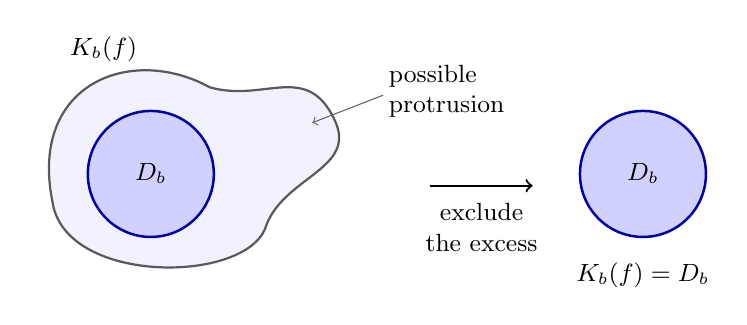
\begin{tikzpicture}[x=1cm,y=1cm,font=\small]
 \filldraw[fill=blue!5,draw=black!65,line width=.8pt]
 (-1.6,-.2) .. controls (-1.9,1.3) and (-.6,1.8) .. (.4,1.25)
 .. controls (1.1,1.05) and (1.65,1.6) .. (2,.8)
 .. controls (2.25,.2) and (1.3,.1) .. (1.1,-.55)
 .. controls (.8,-1.25) and (-1.45,-1.25) .. (-1.6,-.2);
 \filldraw[fill=blue!18,draw=blue!65!black,line width=.9pt]
 (-.35,.15) circle (.8);
 \node at (-.35,.15) {$D_b$};
 \node[above] at (-.95,1.45) {$K_b(f)$};
 \draw[->,black!60] (2.6,1.15)--(1.7,.8);
 \node[right,align=left] at (2.55,1.2) {possible\\protrusion};
 \draw[->,line width=.8pt] (3.2,0)--(4.5,0);
 \node[below,align=center] at (3.85,-.1) {exclude\\the excess};
 \filldraw[fill=blue!18,draw=blue!65!black,line width=.9pt]
 (5.9,.15) circle (.8);
 \node at (5.9,.15) {$D_b$};
 \node[below] at (5.9,-.85) {$K_b(f)=D_b$};
\end{tikzpicture}
\caption{A distinguished disk may initially be only part of a limiting
complementary component. The marked-component argument excludes every
such protrusion. This is a schematic picture; no boundary regularity of
$K_b(f)$ is assumed.}
\label{fig:protrusion}
\end{figure}


\subsection{From finite uniformization to boundary control}

Koebe proved the finite-connectivity theorem; see his 1920 treatment
\cite{Koebe1920}. He and Schramm established the countably connected
case \cite[Theorem~0.1]{HeSchramm1993}. Schramm introduced transboundary
extremal length and gave another proof, as well as uniformization results
for domains bounded by points and $K$-quasicircles for a fixed $K$
\cite{Schramm1995}.  These results combine
finite conformal approximation with estimates controlling which
boundary components survive the limit.

Geometric conditions also yield circle-domain models beyond countable
connectivity.  Esmayli and Rajala proved uniformization for cospread
domains, and more generally under a uniform quasitripod condition and
a packing bound \cite[Theorem~1.3 and Corollary~1.6]{EsmayliRajala2026}.
Karafyllia and Ntalampekos established the conjecture for spherical
Gromov-hyperbolic domains, obtaining uniform circle-domain models and
M\"obius uniqueness \cite[Theorem~1.2]{KarafylliaNtalampekos2024}.
Theorem~\ref{thm:main} imposes no geometric condition on the complement.

Finite approximations alone do not settle the limiting problem.
Rajala showed that arbitrary interior exhaustions can fail to have
circle-domain limits, and proved an exhaustion refinement theorem for
countably connected domains \cite[Theorems~1.1--1.3]{Rajala2025}.
Combining Theorem~\ref{thm:main} with Ntalampekos and Rajala's
exhaustion theorem \cite[Theorem~1.1]{NtalampekosRajala2025} gives an
unconditional fixed-domain approximation: every proper domain
$G\subsetneq\Chat$ has an exhaustion $G_j\subset G_{j+1}$,
$\bigcup_jG_j=G$, by finitely connected domains bounded by finitely many
disjoint Jordan curves lying in $G$. Fix three distinct points
$a_1,a_2,a_3\in G_1$. The conformal uniformizations
$f_j:G_j\to D_j$ onto finitely connected circle domains, normalized by
$f_j(a_k)=a_k$ for $k=1,2,3$, converge locally uniformly in the spherical
metric along the whole sequence to a conformal homeomorphism of $G$
onto a circle domain. For $G=\Chat$, the identity gives the trivial case.
This asserts the existence of a suitable exhaustion, not convergence
for arbitrary exhaustions. For further history, see \cite{Ntalampekos2026}.

We obtain the required control by choosing analytic tests on $G$ before
taking finite uniformizations.  A crucial freedom is to retain the
original conformal structure on each compact core while choosing a new
structure on its finite completion.  The core eventually exhausts the
whole domain, so the limiting map is conformal in the original
structure.  The tests are real functions or functions
with additive period one around a selected component. Each has finite
Dirichlet energy and a square-summable bound on its oscillation at the
complementary components. Small real barriers collapse unmarked
components; period-one tests detect a protrusion beyond a marked disk
through a boundary integral.

The mixed use of domain energy and boundary weights belongs to the
transboundary extremal-length approach introduced by Schramm
\cite{Schramm1995}.  Our path construction charges repeated boundary
visits individually and records portions traveling in earlier level
sets.  The law duality is a form of Fuglede's modulus for measure
systems \cite{Fuglede1957}, with the probability-measure duality
of Ambrosio, Di Marino, and Savar\'e
\cite{AmbrosioDiMarinoSavare2015}.  The additional tasks here are
to fuse the countable tests into one law controlling all boundary components,
to preserve compatibility as tests are appended, and to exclude all
possible noncircular limiting components.

\subsection{Proof overview}

Collapse each complementary component of $G$ to one point. The quotient
$X$ is a topological sphere, and $B=X\setminus G$ is compact and totally
disconnected. Thus $B$ supplies the labels $b$ used above. We use the
topology of $X$ to approach components, while retaining the original
conformal structure on $G$ for length and energy.

Section~\ref{sec:setup} defines the tests and their compatibility
condition. Compatibility controls how the level sets of a new test
meet continua formed from earlier levels. It permits the simultaneous
transfer in Section~\ref{sec:transfer}: finitely many tests extend to a
finite conformal completion, agree with the originals on a prescribed
compact core, and acquire arbitrarily little additional energy or
excess boundary oscillation. Their periods are preserved exactly. The
conformal structure may change outside the core; the cores eventually
exhaust $G$. Finite circle-domain uniformization then produces the
limits and component correspondence described above.

The tests themselves come from a boundary alternative. Either an end
can be separated from a fixed interior anchor by a small compatible
barrier, or there is a probability law of paths from the anchor to that
end with controlled mean arclength occupation. Section~\ref{sec:barriers}
constructs the barriers using paths that may run through complementary
components. Tags record portions lying in previously chosen level sets;
the remaining boundary contacts obey explicit incidence bounds. These
conditions allow paths to be spliced near their ends without losing the
estimates.

Section~\ref{sec:laws} proves the alternative. We use the
modulus--probability duality of Ambrosio, Di Marino, and Savar\'e
\cite{AmbrosioDiMarinoSavare2015}, proving the required measure-family
form in full. This first gives a path law for each prescribed countable
set of boundary tests and each atomless test measure. A separate fusion
argument produces \emph{one} law whose hit probabilities have bounded
counting $\ell^2(B)$ norm on the entire, possibly uncountable, set $B$.
Expected visit counts on previously prescribed countable sets are
controlled separately.

Section~\ref{sec:selection} removes diffuse intersections between
independent path laws. A four-path crossing argument then shows that
only countably many ends can lack small barriers. Selecting countably
many barriers gives a countable marked set $S\subset B$ and collapses
every $K_b(f)$ with $b\notin S$. This conclusion survives every later
countable compatible extension of the tests.

Section~\ref{sec:streams} handles the marked components. Averaging the
integer indices of lifted simple arcs produces period-one tests with
small energy and small oscillation away from the selected end. A
Stokes estimate turns these bounds into an upper bound on a boundary
integral. A protrusion would force a strictly larger lower bound.
Each such test excludes a neighborhood of a possible pair $(f,D_b)$;
second countability permits a countable selection excluding all pairs
with $D_b\ne K_b(f)$. The final simultaneous transfer proves
Theorem~\ref{thm:main}.

Theorem~\ref{thm:retained-tests} records the same construction with
an arbitrary prescribed countable compatible list retained from the outset.
For a finite family of bounded continuous real functions on $X$,
smooth with finite
Dirichlet energy on $G$, the simple sufficient condition
$\area((u_i,u_j)(B))=0$ for distinct tests gives exact agreement on
exhausting cores, vanishing tail energy, and vanishing square-summed
boundary oscillations; see Corollary~\ref{cor:scalar-retained-tests}.
This quantitative conclusion supplies the analytic input for the
removable-boundary rigidity companion \cite{OpenAIRigidity2026}.

Section~\ref{sec:hyperbolic} derives the geometric consequence from
Luo and Wu's Theorem~1.1(a) \cite{LuoWu2024}: every complete hyperbolic
surface of genus zero is intrinsically realized by the boundary of a
hyperbolic convex hull whose ideal set has round-disk or point components.

\subsection{Conventions and classical inputs}

The classical inputs are finite circle-domain uniformization, compact
genus-zero uniformization, Moore's decomposition theorem, area and
coarea, and standard Borel selection and refinement theorems. They are
cited where used. All constructions of compatible tests, fusion of
laws, and component exclusions are proved below.

Path laws are Borel probability measures on the stated code spaces.
We use their completions for universally measurable selections and
analytic events, and take the resulting laws on the Borel
sigma-algebra. Every nonnegative sum over an arbitrary index set is the
supremum of its finite subsums. In particular, every $\ell^2$ function
has countable positive support.

\section{The quotient sphere and compatible coordinates}\label{sec:setup}

We first collapse each complementary component to a point and construct
smooth compact regions exhausting the domain.  We then define
coordinates with controlled boundary oscillation and a
compatibility condition on their level sets.  The last two lemmas give
the level-set geometry and null-image criterion used to establish that
condition.

Throughout, a domain is nonempty, open, and connected.  The case
$G=\Chat$ is immediate, so we assume that the complement is nonempty.
After a M\"obius change of coordinate, we assume that
$\infty\in G$.  Fix $R>0$ such that
\[
 \{z:|z|\ge R\}\cup\{\infty\}\subset G.
\]
We use $\dd s$ and $\dd a$ for spherical length and area on the original
sphere.  We call this the \emph{physical} sphere when distinguishing it
from a quotient introduced below.  The $L^2$ norm of a one-form is its
Dirichlet energy norm; in two dimensions this norm is unchanged by a
conformal change of metric.

\subsection{Collapsing complementary components}

A \emph{continuum} is a nonempty compact connected set; it is
\emph{nondegenerate} if it has more than one point.

\begin{lemma}[The quotient sphere]\label{lem:quotient}
Collapse each component of $\Chat\setminus G$ to a point, and leave
the points of $G$ as singleton decomposition elements.  The resulting
quotient map
\[
 \pi:\Chat\longrightarrow X
\]
is a closed monotone map onto a topological sphere.  Its restriction to
$G$ is a homeomorphism onto an open subset of $X$.  The set
\[
 B=X\setminus\pi(G)
\]
is compact and totally disconnected.  Moreover, the inverse image under
$\pi$ of every continuum in $X$ is connected.
\end{lemma}

\begin{proof}
Put $F=\Chat\setminus G$.  To apply Moore's decomposition theorem,
we check that the decomposition relation is closed and that every
element is nonseparating.  Suppose first that $x_n,y_n$ belong to the
same decomposition element and converge to $x,y$.  If infinitely many
of those elements are singletons, then $x=y$.  Otherwise, after
discarding finitely many terms, let $F_n$ be the component of $F$
containing $x_n,y_n$.  The hyperspace of nonempty compact subsets of
the sphere is compact, so a subsequence of $F_n$ converges in Hausdorff
distance to a nonempty compact set $A\subset F$.  This limit is
connected and contains $x,y$.  Thus $x,y$ lie in one component of $F$,
which proves closedness of the relation.

Now let $Q$ be a component of $F$.  The connected set $G$ lies in one
component of $\Chat\setminus Q$.  Any other component $V$ would be
disjoint from $G$, and its nonempty boundary
would lie in $Q$.  The connected set $Q\cup\overline V\subset F$
would then strictly contain $Q$, a contradiction.  Hence $Q$ is
nonseparating.  Moore's theorem now identifies $X$ with a topological
sphere; see \cite{Moore1925}.  The quotient is closed and has connected
fibers.  Since $G$ is open and saturated, $\pi|_G$ is a homeomorphism
onto an open subset.

It remains to prove the inverse-image assertion and total
disconnectedness of $B$.  Let $A\subset X$ be a continuum.  If
$\pi^{-1}(A)=P\cup Q$ were a separation into disjoint nonempty compact
sets, every fiber over $A$ would lie entirely in one of $P,Q$.
Consequently $\pi(P)$ and $\pi(Q)$ would be disjoint nonempty compact
sets separating $A$, a contradiction.  A continuum contained in $B$
therefore has connected inverse image in $F$, which must lie in a
single component of $F$.
The continuum is consequently a singleton.  Finally, $B$ is the compact
image of $F$.
\end{proof}

We identify $\pi(G)$ with $G$, orient $X$ consistently with the
physical orientation on $G$, and fix a compatible metric $d_X$ on $X$.
Since a nonempty open subset of a sphere contains a nondegenerate
continuum, $B$ has empty interior.  Thus $G$ is dense in $X$.  We refer
to $B$ as the \emph{dust}.

A \emph{dust disk} is a Jordan domain $U\subset X$ whose closure
misses $\infty$ and whose boundary is a smooth physical Jordan curve
in $G$.  Its physical inverse image is exactly the bounded Jordan
domain enclosed by that same curve.  Indeed, the decomposition
elements avoid the curve and cannot cross it, so the two Jordan sides
are saturated.  We shall use the same notation for a dust disk and its
physical inverse image when no confusion can result.

The next lemma supplies small disks around dust points and smooth
contours avoiding prescribed closed sets.  These constructions will
give the compact exhaustion of $G$.

\begin{lemma}[Small disks and contours]\label{lem:dust-disks}
The following assertions hold.
\begin{enumerate}[label=\textup{(\roman*)}]
\item If $F\subset X$ is closed, every nondegenerate continuum contained
in $F\cup B$ is contained in $F$.
\item Suppose that $F\subset X$ is closed and contains $B$, and that
$\{x\}$ is a component of $F$, with $x\ne\infty$.  Every neighborhood
of $x$ contains the closure of a dust disk containing $x$ whose boundary
misses $F$.
\item Let $A$ be a compact relatively clopen subset of $B$, and let
$W\subset X\setminus\{\infty\}$ be open with $A\subset W$.
For every $\eps>0$, there are finitely many dust disks with pairwise
disjoint closures, all contained with their closures in $W$, of
$d_X$-diameter less than $\eps$, whose union contains $A$.
The disks can be required to avoid $B\setminus A$ and to meet $A$.
\item Suppose that finitely many dust disks have closures in a Jordan
domain $V\subset X\setminus\{\infty\}$, and their boundaries avoid a
closed set $F\supset B$.  Their closures can be covered by finitely many
Jordan disks with pairwise disjoint closures in $V$ and smooth
boundaries in $G\setminus F$.
\end{enumerate}
\end{lemma}

\begin{proof}
We use two facts about compact spaces.  First, a component of a compact
Hausdorff space is the intersection of its relatively clopen
neighborhoods.  Second, if $C$ is a continuum and $P$ is a proper
closed subset of $C$, every component of $P$ meets the boundary of $P$
relative to $C$.  Indeed, a component missing that compact boundary
could be separated from it by a relatively clopen subset of $P$.
That subset would be both open and closed in $C$, a contradiction.
The second fact is the boundary-bumping principle.

For \textup{(i)}, suppose a nondegenerate continuum $C\subset F\cup B$
contains $x\notin F$.  Choose $y\in C\setminus\{x\}$ and a small
closed metric neighborhood $N$ of $x$ missing both $F$ and $y$.
The component of $C\cap N$ containing $x$ meets the boundary of $N$
by boundary bumping.  It is therefore a nondegenerate subcontinuum
contained in $B$, contradicting Lemma~\ref{lem:quotient}.

For the remaining parts, we first describe a common contour
construction on the physical sphere.
If $A_0$ is a compact subset of a physical open set $O$ away from
infinity, a smooth cutoff supported in $O$ and equal to one near $A_0$
has a regular level between zero and one.  This level is a compact
smooth one-manifold, so it has finitely many components, each a smooth
Jordan curve.  The corresponding superlevel set contains $A_0$ and
has compact closure in $O$.  Taking its outer boundary curves fills
its holes.  If $O\subset\pi^{-1}(V)$ for a Jordan domain
$V\subset X\setminus\{\infty\}$, each filled outer contour still
lies in $\pi^{-1}(V)$.  Indeed,
$\pi^{-1}(X\setminus V)$ is connected by
Lemma~\ref{lem:quotient}, contains infinity, and misses the contour;
it must therefore lie on its unbounded side.

For \textup{(ii)}, take a Jordan neighborhood $V$ of $x$
whose closure is inside the prescribed neighborhood and misses
infinity.  By the first compact-space fact above, there is a
compact relatively clopen set $A_0\subset F$ with
$x\in A_0\subset V$.  Choose a physical open neighborhood of
$\pi^{-1}(A_0)$ compactly contained in
\[
 \pi^{-1}(V)\setminus\pi^{-1}(F\setminus A_0).
\]
Apply the contour construction there.  Its boundary curves miss
$\pi^{-1}(F)$.  The connected fiber $\pi^{-1}(x)$ lies
inside one of the resulting outer contours.  Its filled disk projects
to the required dust disk.  Its closure is contained in $V$ by the
connected-complement observation above.

For \textup{(iii)}, the compact metric totally disconnected space $B$
has a clopen base.  Partition $A$ into finitely many compact relatively
clopen pieces $A_1,\ldots,A_m$, each contained in a Jordan neighborhood
$V_i$ with closure in $W\setminus(B\setminus A)$ and diameter less
than $\eps$.  The compact physical preimages of these pieces are
pairwise disjoint.  They therefore have pairwise disjoint open
neighborhoods with disjoint compact closures, each lying in
$\pi^{-1}(V_i)$ and avoiding $\pi^{-1}(B\setminus A_i)$.
Make physical contours inside these neighborhoods.  The boundary
curves obtained for all pieces are mutually disjoint and miss the
whole physical complement of $G$.  Their filled disks are either
nested or have disjoint closures.  Discard the nested ones and any
disk missing $A$.  The remaining disks still cover $A$, have disjoint
closures, and each stays inside its corresponding $V_i$.

For \textup{(iv)}, let $Q$ be the union of the given closed disks.
Its boundary is contained in the union of the given boundaries and
hence misses $F$.  Use the regular-level construction to smooth a
sufficiently small physical outer neighborhood of $\pi^{-1}(Q)$.
Take the smoothing collar around the boundary of $\pi^{-1}(Q)$
disjoint from $\pi^{-1}(F)$ and keep the neighborhood's closure in
$\pi^{-1}(V)$.  There are finitely many smooth boundary
curves by the compact one-manifold argument above.  Fill the outer
contours and discard nested contours.
The connected-complement observation keeps all filled disks in $V$,
and all new boundaries remain in $G\setminus F$.
\end{proof}

We now use part \textup{(iii)} to fix the compact exhaustion.
Additional closed obstacles can be avoided by choosing $W$ disjoint
from them, and each new cover can have its closures inside the
preceding disks.  Choose cores
\[
 K_j=X\setminus\bigcup_{U\in\mathcal U_j}U,
 \qquad K_j\subset\operatorname{int}_X K_{j+1},
 \qquad \bigcup_{j\ge1}K_j=G,
\]
where each $\mathcal U_j$ is a finite family of dust disks with
pairwise disjoint closures, covers $B$, lies on the bounded side of
$|z|=R$, and has mesh tending to zero.  Here the mesh is the maximum
of the $d_X$-diameters of the disks in the cover.  Each $K_j$ is a
compact smooth bordered region in $G$ containing infinity in its
interior.  Every compact subset of $G$ lies in the interior of all
sufficiently large cores.  For $b\in B$, write
\[
 U_j(b)\in\mathcal U_j,\qquad b\in U_j(b),
 \qquad C_j(b)=\partial U_j(b).
\]
Then
\[
 \overline{U_{j+1}(b)}\subset U_j(b),
 \qquad \bigcap_j\overline{U_j(b)}=\{b\}.
\]
Smooth intermediate curves and compact physical collars can be chosen
between successive boundary curves.  We sometimes call the curves
$C_j(b)$ themselves collars; an actual annular neighborhood will always
be specified when one is needed.

\subsection{Coordinates, bands, and compatibility}

We next specify the functions to be transferred from these cores.
For each function, we record its region of definition, any additive
period, and bounds on its energy and limiting oscillation.
Compatibility will constrain how the level sets of different
coordinates can meet at the dust.

Every nonnegative sum indexed by an arbitrary set is understood as
the supremum of its finite subsums.  In particular,
\[
 \|a\|_{\ell^2(B)}^2=\sum_{s\in B}a(s)^2.
\]
A nonnegative $\ell^2(B)$ function has countable positive support.

\begin{definition}[Coordinates]\label{def:coordinates}
A coordinate $u_i$ comes with a closed set $M_i\subset X$, called its
\emph{mask}, and has one of the following forms.
\begin{enumerate}[label=\textup{(\roman*)}]
\item A bounded smooth real function on $G$, with mask $M_i=X$.
\item A coordinate with additive period one, with mask
$M_i=\overline U$ for a dust disk $U$ and singular point
$p_i\in B\cap U$.  On the cyclic universal cover of
$\overline U\setminus\{p_i\}$, it is a smooth real function over
$G\cap M_i$, smooth up to the boundary curve, satisfying
\[
 u_i(Tx)=u_i(x)+1
\]
for the positive deck transformation $T$.
\end{enumerate}
In both cases the differential is single-valued and is required to
satisfy
\[
 \|\dd u_i\|_{2,G\cap M_i}<\infty.
\]
For a nonsingular point $s\in B\cap M_i$, choose a local lift in the
periodic case and define
\[
 I_i(s)=
 \left[\liminf_{\substack{x\to s\\x\in G\cap M_i}}u_i(x),
       \limsup_{\substack{x\to s\\x\in G\cap M_i}}u_i(x)\right].
\]
We call $I_i(s)$ the \emph{band} at $s$ and require it to be a bounded
interval with length at most $a_i(s)$, where $a_i\ge0$ belongs to
$\ell^2(B)$.
For a coordinate with period, set $a_i(p_i)=1$; no real band is
required there.  Set $a_i=0$ off the mask.  A change of local sheet
translates a band by an integer.

A finite or countable well-ordered list of coordinates carries a
countable flag set $\Sigma\subset B$ containing every positive
support $\{a_i>0\}$.  Points of $B\setminus\Sigma$ are called
\emph{free}.  Every coordinate defined at a free point has a unique
trace there, interpreted modulo an integer in the periodic case.
\end{definition}

To include dust points in the level sets, write $\T=\R/\Z$ for the
circle of levels.  For $t\in\T$, let $H_i(t)\subset M_i$ consist of
the domain points with $u_i=t\pmod{1}$, the nonsingular dust points
whose bands project to sets containing $t$ in $\T$, and the singular
point, if present.  Thus the singular point belongs to every level.
We use Haar measure of total mass one on $\T$ and product Haar
measure on tuples.  Thus
\begin{equation}\label{eq:band-incidence}
 \bigl|\{t\in\T:s\in H_i(t)\}\bigr|
 \le \min\{1,a_i(s)\}\le a_i(s)
 \qquad(s\in B).
\end{equation}

Before stating compatibility, we record that each level graph
\[
 \{(s,t)\in X\times\T:s\in H_i(t)\}
\]
is compact.  At a nonsingular dust point, the lower band endpoint is
lower semicontinuous and the upper endpoint is upper semicontinuous,
as follows directly from their neighborhood-infimum and
neighborhood-supremum definitions.  The local boundedness furnished
by a finite band also bounds all nearby bands in a common lift.
These facts give closedness at nonsingular dust points.  Smoothness
gives closedness at domain points, and the definition includes every
limiting level at a singular point.  Since the mask is closed, the
graph is closed in the compact space $X\times\T$.

\begin{definition}[Compatibility]\label{def:compatibility}
A well-ordered list with its flag set satisfies \textup{(P)} if, for
each label $j$, each nonempty finite list of lower labels
$i_1,\ldots,i_d<j$ \emph{with repetitions permitted}, and almost every
$(t,t_1,\ldots,t_d)\in\T^{d+1}$, no free point of $H_j(t)$ belongs
to a nondegenerate component of
\[
 H_{i_1}(t_1)\cup\cdots\cup H_{i_d}(t_d).
\tag{P}
\]
\end{definition}

The null-set assertion uses completed product measure.  To justify
its measurability, consider the compact hyperspace of nonempty
subcontinua of $X$.  The conditions that a continuum contain a
specified point, lie in a specified finite level
union, and have diameter at least $1/n$ are closed conditions on the
continuum, point, and level tuple.  Projection over that compact
hyperspace is closed.  Taking the union over $n$ shows that belonging
to a nondegenerate component of the level union is a Borel relation
in the point and tuple.  Requiring the point to be free is Borel, and
projection over the point makes the failure relation in
Definition~\ref{def:compatibility} analytic.  It is therefore
universally measurable.  In particular, we may prove \textup{(P)} by
slicing in its level parameters; see \cite{Kechris1995}.

Increasing $\Sigma$ preserves \textup{(P)}, as does passage to a
finite ordered sublist with the same flags.  At a countable limit
stage we take the union of the lists and of their flag sets.  Every
condition in \textup{(P)} involves only finitely many coordinates,
so previously established compatibility persists at such a stage.

\subsection{The geometry of generic level unions}

Compatibility concerns nondegenerate components of finite level
unions.  We show that almost every such union has only countably many
of these components and that its subcontinua are locally connected.
The proof uses finite physical length in $G$ to control continua of
fixed positive diameter in $X$.

We write $\HH^1_{\mathrm{sph}}$ for one-dimensional Hausdorff measure
with respect to the spherical metric.

\begin{lemma}[Generic level continua]\label{lem:level-continua}
For each finite list $i_1,\ldots,i_d$, almost every tuple
$(t_1,\ldots,t_d)$ gives a compact level union
\[
 H=\bigcup_{k=1}^d H_{i_k}(t_k)
\]
with the following properties.
\begin{enumerate}[label=\textup{(\roman*)}]
\item $\HH^1_{\mathrm{sph}}(H\cap G)<\infty$.
\item For each $\eps>0$ there is a finite bound on the cardinality of
any family of pairwise disjoint subcontinua of $H$ having
$d_X$-diameter at least $\eps$.
\item $H$ has at most countably many nondegenerate components, and
every subcontinuum of $H$ is locally connected.  Any two distinct
points in a connected relatively open subset of such a subcontinuum
can be joined by a simple arc within that subset.
\end{enumerate}
In addition, if $q\ge0$ is Borel on $G$ and $m\ge0$ is in
$\ell^2(B)$, then for each label $i$,
\begin{equation}\label{eq:weighted-level-bound}
 \begin{split}
 &\int_{\T}\left(
   \int_{H_i(t)\cap G}q\,\dd\HH^1_{\mathrm{sph}}
   +\sum_{s\in H_i(t)\cap B}m(s)\right)\dd t\\
 &\hspace{15mm}\le
   \int_{G\cap M_i}q|\dd u_i|\,\dd a
   +\sum_{s\in B}m(s)a_i(s).
 \end{split}
\end{equation}
The right side is finite when $q\in L^2(G,\dd a)$.
\end{lemma}

\begin{proof}
We first prove the weighted estimate and finite length, then derive
the topological conclusions from that length bound.
Apply the coarea formula to the smooth circle-valued map
$u_i\pmod1$ on its masked domain; see \cite{Federer1969}.
Mask-boundary portions contribute zero after integration in the level
parameter: each point of that smooth boundary occurs at just one
level.  Thus the domain term in
Equation~\eqref{eq:weighted-level-bound} equals its stated area
integral.  The dust term is bounded by
Equation~\eqref{eq:band-incidence} and Tonelli's theorem; only the
countable support of $m$ is involved.  Cauchy--Schwarz bounds the
right side when $q\in L^2$.  Taking $q=1$ and $m=0$ gives finite
length for almost every level, since the spherical area is finite.
Summing over the finite list proves \textup{(i)}.

For \textup{(ii)}, only compactness of $H$ and the finite length in
\textup{(i)} are needed.  Fix $\eps>0$ and choose a core $K$ whose
complementary dust disks have
$d_X$-diameter less than $\eps$.  Every continuum $Q\subset H$ with
$\diam_X Q\ge\eps$ meets $K$: otherwise its connectedness places it
inside one of those disjoint disks.  Compactness of the physical set
$K\subset G$ and uniform continuity of $\pi$ give $r>0$ such that
every closed spherical $r$-ball centered on $K$ is contained in $G$
and has image of $d_X$-diameter less than $\eps$.  Decrease $r$ so
these balls are ordinary embedded spherical disks.

Choose $p\in Q\cap K$.  Since the closed spherical $r$-ball about
$p$ has quotient diameter less than $\eps$, $Q$ exits this ball.
By boundary bumping, the component of the intersection containing
$p$ meets the ball boundary.  Spherical distance from $p$, a
$1$-Lipschitz function, maps this subcontinuum onto $[0,r]$.  Therefore
\[
 \HH^1_{\mathrm{sph}}(Q\cap G)\ge r.
\]
For pairwise disjoint continua these measures add.  Their number is
at most $\HH^1_{\mathrm{sph}}(H\cap G)/r$, proving \textup{(ii)}.

The bound in \textup{(ii)} now gives \textup{(iii)}.
For each $n$ there are only finitely many components
of $H$ with diameter at least $1/n$, proving countability of the
nondegenerate components.  For local connectedness of every
subcontinuum, let $L\subset H$ be any subcontinuum, let
$p\in L$, and take a sufficiently small radius $t>0$.  Let $A$ be
the component through $p$ of $L\cap\overline B_X(p,t)$.  If $A$
were not a relative neighborhood of $p$ in $L$, there would be points
$p_n\to p$ in other components of this closed intersection.  After
passing to a subsequence those components are distinct: a finite
union of components not containing $p$ is compact and misses $p$.
If the closed intersection is all of $L$, it has only one component,
so this case is already excluded.  Boundary bumping now shows that
each of the distinct components meets $\{x:d_X(x,p)=t\}$.  For large
$n$ it consequently has diameter at least $t/2$, in contradiction to
\textup{(ii)}.  Hence $A$ is a connected neighborhood of $p$.
Arbitrarily small choices of $t$ prove that $L$ is locally connected.

Finally, a connected open subset $V$ of a locally connected metric
continuum is arcwise connected.  One can see path connectedness
directly by chaining connected relatively open sets of small diameter
with closures in $V$, and then recursively refining each link inside
its predecessor.  Connectedness guarantees finite chains between
specified endpoints at every refinement.  Choose the parameter
subdivisions and image diameters to tend to zero.  Completeness gives
a continuous path between the endpoints whose image remains in $V$.
The elementary loop-erasure theorem for a path in a Hausdorff space
then supplies a simple arc with the same endpoints inside its image.
These standard continuum facts are also recorded in
\cite{Whyburn1942}.
\end{proof}

We have proved that generic level continua admit simple arcs locally.
The next lemma converts bounds along such arcs into null images of
traces, which will establish compatibility.  The use of outer measure
requires no measurability of the trace function.

\begin{lemma}[A null image criterion for traces]\label{lem:trace-null}
Let $L$ be a locally connected metric continuum, let $V\subset L$
be relatively open, and let $\nu$ be a finite Borel measure on $L$.
Suppose $F\subset V$ has $\nu$-outer measure zero and a function
$v:F\to\R$ satisfies
\[
 |v(x)-v(y)|\le A\nu(\alpha)
\]
for some finite $A\ge0$, every $x,y\in F$, and every simple arc
$\alpha\subset V$ joining $x$ and $y$.  Then $v(F)$ has Lebesgue
outer measure zero.

The same conclusion holds locally when $F$ is covered by countably
many such relatively open sets and $v$ has a real branch on each.
In particular, the corresponding image in $\T$ has Haar measure
zero for a circle-valued trace with these local branches.
\end{lemma}

\begin{proof}
For $\delta>0$, regularity of the finite Borel measure on the compact
metric space $L$ gives a relatively open set $O$ with
\[
 F\subset O\subset V,\qquad \nu(O)<\delta.
\]
Local connectedness makes each component $O_k$ of $O$ relatively
open.  There are at most countably many components, because disjoint
nonempty open sets in a second-countable space are countable.
Any two points of $F\cap O_k$ can be joined by a simple arc in $O_k$.
Consequently
\[
 \diam v(F\cap O_k)\le A\nu(O_k).
\]
Cover these real images by intervals, allowing arbitrarily small
summable excess lengths.  Countable subadditivity gives
\[
 |v(F)|^*\le A\sum_k\nu(O_k)=A\nu(O)\le A\delta.
\]
Letting $\delta$ tend to zero proves the first assertion.  Apply it
separately to the countably many local branches for the second.
\end{proof}

\section{Finite transfer and normalized limits}\label{sec:transfer}

We now transfer finitely many compatible coordinates to a smooth surface
with finitely many holes.  The transfer preserves the coordinates and the
original conformal structure near a prescribed compact core.  Outside the
core we choose the coordinates and the conformal structure together, so
that the added energy and the excess over the given oscillation budgets
are small.  The key is to make pairwise wedge products small: a suitable
metric then makes the sum
of the coordinate energies small as well.

After proving this finite construction, we normalize its circle-domain
maps and pass to limits on $G$.  Nested source collars will identify all
complementary components of the limit and locate the round disks
associated with prescribed dust points.

\subsection{The transfer theorem}

The construction selects finitely many disjoint dust disks.  Some are
filled, with a conformal structure chosen below; the others have their
interiors excised and are called \emph{terminal disks}.  Each terminal
disk is indexed by a distinct dust point in its interior.

In expressions involving a physical completion, we use the same symbol
$M_i$ for the inverse image $\pi^{-1}(M_i)$ of a mask in $X$.
Thus $Q\cap M_i$ below is a subset of the physical sphere.

\begin{theorem}[Finite transfer]\label{thm:transfer}
Let $u_1,\ldots,u_m$ be a finite ordered list satisfying
Definition~\ref{def:coordinates} and compatibility~(P), with a common
countable flag set $\Sigma$.  The same assertion holds for a finite
ordered sublist of a countable compatible list.  Prescribe a finite set
$F\subset B$ containing all singular points of the list, a compact core
$K_0\subset G$, a dust-disk cover from the fixed exhaustion, and
$\eps>0$.

There exist a smooth compact core $K\subset G$, finitely many
terminal disks $T_s$ with pairwise disjoint closures, indexed by a finite set
$S\subset B$ containing $F$, and a smooth metric $g$ on the physical
sphere, with the following properties.  Every terminal disk lies in a
member of the prescribed cover, $s\in T_s$, and $K$ contains $K_0$ and
all mask boundaries in its interior.  The metric $g$ agrees with the
spherical metric on a neighborhood of $K$.  Write
\[
 Q=\Chat\setminus\bigcup_{s\in S}T_s,
 \qquad Q^\circ=\Chat\setminus\bigcup_{s\in S}\overline{T_s}.
\]
Then $K\subset Q^\circ$, and $Q$, equipped with $g$, is a smooth
bordered surface of genus zero.
Each $u_i$ has a transferred coordinate $u_i^*$ on $Q\cap M_i$, smooth
up to its boundary in local real branches, with the following properties.
\begin{enumerate}[label=\textup{(\roman*)}]
\item $u_i^*=u_i$ on a neighborhood of $K\cap M_i$;
\item The total energy outside $K$ satisfies
\begin{equation}\label{eq:transfer-tail}
 \sum_{i=1}^m
 \|\dd u_i^*\|_{2,(Q\setminus K)\cap M_i,g}^2<\eps^2;
\end{equation}
\item For each nonsingular terminal index $s\in S\cap M_i$, a
single-valued lift on a collar of $\partial T_s$ has boundary oscillation
$A_i(T_s)$ satisfying
\begin{equation}\label{eq:transfer-oscillation}
 \left(\sum_{\substack{s\in S\cap M_i\\s\ne p_i}}
       [A_i(T_s)-a_i(s)]_+^2\right)^{1/2}<\eps.
\end{equation}
Here $[x]_+=\max\{x,0\}$.  For a real coordinate the restriction
$s\ne p_i$ is omitted.
\item A periodic coordinate still adds $1$ under its positive deck
translation.  Its differential has period $1$ around the terminal disk
indexed by its singular point, and period $0$ around every other
terminal disk in its mask.  Here a positive circuit around a terminal
disk is counterclockwise around that disk.
\end{enumerate}
The core $K_0$ may contain any prescribed compact subsets of $G$.
In particular the conformal structure on $\{|z|\ge R\}$ can always be
retained.  Terminal disks can be required to lie in arbitrarily small
prescribed dust neighborhoods of their indices.
\end{theorem}

\begin{proof}
We first replace the coordinates outside a large core by shifted
staircases.  Compatibility will provide disks on whose collars at most
one staircase varies.  We can then fill those disks so that the extended
differentials have rank at most one, and choose a metric from these
differentials.

We regard $\dd u_i$ as zero wherever its mask is absent; every use of
this convention is away from mask boundaries.  Fix $\eta>0$, to be
chosen in terms of $\eps$ at the end.

\smallskip\noindent
\emph{Step 1: random staircases.}
Choose a smooth core $K$ containing $K_0$, all mask boundaries, and the
exterior $\{|z|\ge R\}$ in its interior.  Enlarge it until the original
energies outside $K$ are so small that
\begin{equation}\label{eq:transfer-original-wedges}
 \sum_{i<j}\int_{G\setminus K}
       |\dd u_i\wedge\dd u_j|
 \le \sum_{i<j}
       \|\dd u_i\|_{2,G\setminus K}
       \|\dd u_j\|_{2,G\setminus K}
 <\frac{\eta}{8}.
\end{equation}
The mask intersections are implicit in these integrals.  Take
$\chi\in C^\infty(G,[0,1])$ equal to $0$ on a
neighborhood of $K$ and equal to $1$ outside a larger compact set.

The staircases will vary only near a finite grid of levels modulo one.
Let $h=1/N$, where $N$ is a positive integer.  Independently for each
$i$, choose $\theta_i$ uniformly in $[0,h)$.  For $0<\delta<h/4$ take a
smooth nondecreasing staircase $P_{i,\delta}$ with
\[
 P_{i,\delta}(x+h)=P_{i,\delta}(x)+h,
 \qquad |P_{i,\delta}(x)-x|\le h,
\]
whose derivative is supported within distance $\delta$ of
$\theta_i+h\Z$.  It is obtained by translating one fixed staircase
with an $h$-periodic derivative of integral $h$ over a period.  Therefore
\begin{equation}\label{eq:transfer-staircase-mean}
 \E P_{i,\delta}'(x)=1
 \quad\text{for every }x.
\end{equation}
Because $1=Nh$, it also satisfies
$P_{i,\delta}(x+1)=P_{i,\delta}(x)+1$.

Use the cutoff to join each staircase to the original coordinate:
\begin{equation}\label{eq:transfer-staircase}
 v_{i,\delta}
 =u_i+\chi\bigl(P_{i,\delta}(u_i)-u_i\bigr).
\end{equation}
The formula is interpreted in local branches and respects integer
translations, so it is consistent for periodic coordinates.  Set
\[
 q_{i,\delta}=1-\chi+\chi P_{i,\delta}'(u_i),
 \qquad r_{i,\delta}=P_{i,\delta}(u_i)-u_i.
\]
Then $q_{i,\delta}\ge0$, $|r_{i,\delta}|\le h$, and
\[
 \dd v_{i,\delta}
 =q_{i,\delta}\,\dd u_i+r_{i,\delta}\,\dd\chi.
\]
Equation~\eqref{eq:transfer-staircase-mean} and independence for distinct
labels give $\E q_{i,\delta}=1$ and
$\E(q_{i,\delta}q_{j,\delta})=1$ for $i\ne j$.  Consequently the wedge
sum
\[
 W_\delta
 =\sum_{i<j}\int_{G\setminus K}
             |\dd v_{i,\delta}\wedge\dd v_{j,\delta}|
\]
satisfies
\begin{equation}\label{eq:transfer-wedge-mean}
 \E W_\delta
 \le \sum_{i<j}\int_{G\setminus K}|\dd u_i\wedge\dd u_j|
   +(m-1)h\sum_i\int_{\supp\dd\chi}
                         |\dd\chi|\,|\dd u_i|\,\dd a.
\end{equation}
The last integrals are finite because $\supp\dd\chi$ is compact in
$G$.  With $K$ and $\chi$ fixed, choose $h$ small enough that the
right side is less than $\eta/4$, uniformly in $\delta$.

\smallskip\noindent
\emph{Step 2: choosing the grids and terminal indices.}
For the random shifts above, put
\[
 F_i^{\rm grid}
   =\bigcup_{k=0}^{N-1}H_i(\theta_i+kh).
\]
Each grid is compact.  In addition to $F$, retain as terminal indices
all flagged points lying in the grids of two distinct labels:
\[
 S=F\cup
 \bigcup_{i<j}\bigl(\Sigma\cap F_i^{\rm grid}
                                  \cap F_j^{\rm grid}\bigr),
 \qquad J=|S|.
\]
At a nonsingular dust point, a band of length at most $a_i(s)$ meets
the translated lattice with probability at most
$\min(1,a_i(s)/h)$.  The same bound holds at the singular point because
there $a_i(s)=1$.  Thus, by independence,
\begin{equation}\label{eq:transfer-terminal-mean}
 h^2\E J
 \le h^2|F|+
       \sum_{i<j}\sum_{s\in\Sigma}
                 \min(h,a_i(s))\min(h,a_j(s))
 \longrightarrow0\qquad(h\downarrow0).
\end{equation}
Each summand tends to zero and is bounded by $a_i(s)a_j(s)$, whose
sum is finite by Cauchy--Schwarz.  Dominated convergence proves the
limit.  The same estimate gives $J<\infty$ almost surely for each $h$.

Decrease $h$, if necessary, so that $h^2\E J<\eta^2/4$ as well.
Fix a deterministic sequence $\delta_k\downarrow0$ with
$\delta_k<h/4$.  Fatou's Lemma and
Equation~\eqref{eq:transfer-wedge-mean} give
\[
 \E\bigl(\liminf_{k\to\infty}W_{\delta_k}\bigr)<\eta/4.
\]
Markov's inequality shows that a set of positive probability satisfies
both
\begin{equation}\label{eq:transfer-grid-selection}
 \liminf_{k\to\infty}W_{\delta_k}<\eta,
 \qquad h\sqrt J<\eta.
\end{equation}

We also require compatibility~(P) for every choice of one lattice
level for each of any collection of distinct labels.  Each such tuple
has an absolutely continuous distribution in its level variables, and
there are only finitely many choices.  Hence this additional requirement
has probability one.  Fix grids satisfying it and
Equation~\eqref{eq:transfer-grid-selection}.

The grids and their finite set $S$ are now fixed.  Choose terminal
disks about the points of $S$, with pairwise disjoint closures, in the
region where $\chi=1$.  They contain no other
point of $S$, lie in the prescribed dust neighborhoods, and avoid all
mask boundaries.  For every nonsingular coordinate present at $s$, its
values in a sufficiently small neighborhood of $s$, in an appropriate
local lift, lie in its band enlarged by $h$ at each end.  We therefore
choose $T_s$ so that
\[
 \osc_{\partial T_s}u_i\le a_i(s)+2h.
\]
The bound $|P_{i,\delta}(x)-x|\le h$ gives, simultaneously for every
$\delta$,
\begin{equation}\label{eq:transfer-terminal-oscillation}
 \osc_{\partial T_s}v_{i,\delta}\le a_i(s)+4h.
\end{equation}
No real oscillation bound is required at a singular index.  The
terminal disks are now fixed, while the staircase width can still
decrease.

\smallskip\noindent
\emph{Step 3: filling disks whose boundaries meet at most one grid.}
We claim that the remaining dust has a finite cover by disks, with
pairwise disjoint closures and disjoint from the terminal disks, such
that the boundary of each new disk meets at most one
$F_i^{\rm grid}$.  All these disks can be placed where $\chi=1$,
inside the prescribed dust neighborhoods, and away from mask
boundaries.

First observe that if $s\in B\cap F_j^{\rm grid}$ is not a terminal
index, then $s$ is a singleton component of
\begin{equation}\label{eq:transfer-lower-obstacle}
 B\cup\bigcup_{i<j}F_i^{\rm grid}.
\end{equation}
If $s$ is flagged, it does not belong to any lower grid, by the choice
of $S$.  If $s$ is free, each coordinate defined at $s$ has a unique
trace.  Thus, near $s$, only one level from each of the grids occurring
at $s$ can be present; the other levels are closed and miss $s$.
If a nondegenerate component of the lower grid union contained $s$,
intersect that component with a sufficiently small closed neighborhood
of $s$.  Boundary bumping makes the component of this intersection
through $s$ nondegenerate.  It uses only the lower levels present at
$s$, contradicting the chosen instance of compatibility~(P).
Lemma~\ref{lem:dust-disks}\textup{(i)} shows that adjoining $B$ cannot
create another nondegenerate continuum through $s$.  This proves the
singleton assertion in both cases.

Process the labels in decreasing order.  At the stage for $j$, the
remaining dust is a compact relatively clopen subset of $B$, disjoint
from the already chosen closed disks and from every higher grid.  Use
Lemma~\ref{lem:dust-disks} to cover it by finitely many disjoint small
preliminary disks whose closures avoid these obstacles.  In each such
disk $V$, the remaining points of $F_j^{\rm grid}\cap B$ form a
compact set.  Each is a singleton component of the closed set in
Equation~\eqref{eq:transfer-lower-obstacle}; hence
Lemma~\ref{lem:dust-disks} encloses it in a smaller disk with closure
in $V$ and boundary avoiding that closed set.

Take finitely many such disks covering the compact target.  To merge
them while preserving boundary avoidance, perturb their
finitely many smooth boundaries into general position within the open
complement of the obstacle, take the outer contours of their union,
and smooth the corners there.  Fill bounded complementary regions and
discard nested contours.  Every resulting disk stays in $V$, because
the complement of $V$ is connected and contains infinity.  The
resulting closures are pairwise disjoint, their interiors still cover
the target, and their boundaries avoid all lower grids.  They also
avoid the higher grids, since their closures lie in $V$.  Add these
disks to the chosen collection and continue.  After the last label,
cover the dust still remaining by disks avoiding all the grids.  This
proves the claim.  Call all disks chosen in this step
\emph{filling disks}.

\smallskip\noindent
\emph{Step 4: smooth fillings of rank at most one.}
The finite collection of terminal and filling disks covers $B$ in its
interiors.  Its complement is therefore a compact subset of $G$.
On each filling boundary, every coordinate except possibly one avoids
its grid.  Choose connected collars, compact in $G$, on which this
avoidance still holds and $\chi=1$.  Every singular point lies in its
assigned terminal disk, so the coordinates have single-valued lifts on
each filling collar.  When the collar avoids $F_i^{\rm grid}$, a real
lift has connected image in one interval complementary to the level
lattice $\theta_i+h\Z$.  Compactness of the collar
then makes its staircase constant for all sufficiently small $\delta$.
Call these constant coordinates inactive on the collar.  There are
only finitely many collars, so one width bound works for all of them.

By Equation~\eqref{eq:transfer-grid-selection} we may choose one of the
$\delta_k$ small enough for all these collar conditions and with
$W_{\delta_k}<\eta$.  Fix this width and suppress it from the notation.
Retain $v_i$ on the complement of the selected disks.  Across each
filling disk extend the inactive coordinates constantly.  Extend the
one possibly varying coordinate from an inside collar by a smooth
cutoff, making it constant on a smaller interior disk.  These
extensions agree with the retained coordinates on full collars and
are therefore smooth.  Their differentials have rank at most one
at every point of a filling disk, so
\begin{equation}\label{eq:transfer-filling-wedges}
 \dd u_i^*\wedge\dd u_j^*=0
 \quad\text{on every filling disk.}
\end{equation}
Here $u_i^*$ denotes the resulting coordinate on the completed
bordered surface $Q$.

To check the periods, pull back by $\pi$ the cyclic cover of the
punctured mask.  This cover is trivial on each filling disk.  Perform
the extension on one sheet and use its integer translates on the
others.  Equation~\eqref{eq:transfer-staircase} respects the same
translations, so the completed coordinate has its original additive
period.  Under $\pi$, a counterclockwise circuit about $T_{p_i}$ winds
once about $p_i$, while a circuit about any other terminal disk in the
mask has winding number zero.  Thus the periods are exactly those
asserted in the theorem.

\smallskip\noindent
\emph{Step 5: choosing a metric.}
The coordinates are now extended, with small wedge integrals outside
$K$ and zero wedge products in the filling disks.  It remains to turn
this control into small energy in one smooth metric.
Let $g_0$ be the spherical metric and, outside $K$, form the smooth
positive semidefinite tensor
\[
 A=\sum_{i:\,M_i\text{ present}}\dd u_i^*\otimes\dd u_i^*.
\]
The sum at a point includes the masks containing that point.  All mask
boundaries lie inside $K$, so this tensor is smooth where it is used.
The differentials are single-valued even for periodic coordinates.
For $\tau>0$ put
$g_\tau=A+\tau g_0$.  In a $g_0$-orthonormal frame, let
$\lambda_1,\lambda_2\ge0$ be the eigenvalues of $A$.  The sum of the
energy densities of the coordinates in $g_\tau$, expressed relative
to $\dd a_{g_0}$, is
\begin{equation}\label{eq:transfer-metric-density}
 \operatorname{tr}(g_\tau^{-1}A)\sqrt{\det g_\tau}
 =\frac{2\lambda_1\lambda_2+\tau(\lambda_1+\lambda_2)}
        {\sqrt{(\lambda_1+\tau)(\lambda_2+\tau)}}
 \longrightarrow 2\sqrt{\lambda_1\lambda_2}.
\end{equation}
In particular the limit is zero when $A$ has rank at most one.
The Cauchy--Binet identity gives
\[
 \det A=\sum_{i<j}|\dd u_i^*\wedge\dd u_j^*|_{g_0}^2.
\]
The transferred differentials are bounded on the finitely many smooth
compact pieces of the completed surface.  The densities in
Equation~\eqref{eq:transfer-metric-density} therefore have a common
integrable bound for $0<\tau\le1$: each term
$\lambda_1\sqrt{(\lambda_2+\tau)/(\lambda_1+\tau)}$ is at most
$\sqrt{\lambda_1(\lambda_2+1)}$, and similarly for the other term.
Dominated convergence is therefore applicable.  By
Equation~\eqref{eq:transfer-filling-wedges} and the choice of the width,
\begin{equation}\label{eq:transfer-optimized-energy}
 \lim_{\tau\downarrow0}
       \sum_i\|\dd u_i^*\|_{2,(Q\setminus K)\cap M_i,g_\tau}^2
 =2\int_{Q\setminus K}\sqrt{\det A}\,\dd a_{g_0}
 \le2W_\delta<2\eta.
\end{equation}

Choose $\tau$ so that the total energy outside $K$ in $g_\tau$ is
less than $3\eta$.  With this regularization fixed, interpolate between
$g_0$ and $g_\tau$ in a thin exterior collar of $\partial K$, keeping
$g_0$ on a neighborhood of $K$.  The interpolated metrics are uniformly
positive definite and their energy densities are bounded on the
collar.  We may therefore choose its thickness so that the
interpolation adds less than $\eta$ to the total energy.  Extend the
resulting metric smoothly across each terminal cap, first across its
collar and then by interpolation with $g_0$ inside the cap.  This
does not change the metric on $Q$.

The tail energy is now less than $4\eta$.  Moreover,
Equation~\eqref{eq:transfer-terminal-oscillation} gives for each $i$
\[
 \left(\sum_{s\ne p_i}[A_i(T_s)-a_i(s)]_+^2\right)^{1/2}
 \le4h\sqrt J<4\eta.
\]
Taking $\eta<\min(\eps^2/4,\eps/4)$ establishes
Equations~\eqref{eq:transfer-tail} and
\eqref{eq:transfer-oscillation}.  All alterations occurred outside a
neighborhood of $K$, completing the proof.
\end{proof}

We will also need energy control away from a prescribed part of the
core.  Exact agreement on $K$ and the tail estimate give, for every
measurable $E\subset K\cap M_i$,
\begin{equation}\label{eq:transfer-localized-energy}
 \|\dd u_i^*\|_{2,(Q\cap M_i)\setminus E,g}^2
 \le \|\dd u_i\|_{2,(G\cap M_i)\setminus E}^2+\eps^2.
\end{equation}
Both this estimate and the boundary oscillation estimates are unchanged
by a conformal uniformization of $Q^\circ$.

\subsection{Circle-domain completions and compactness}

We now apply finite uniformization to these completions and obtain a
subsequential limit on the original domain.  Keeping a fixed exterior
region unchanged will give one normalization and one bound for all
the finite maps.

Extend the metric of Theorem~\ref{thm:transfer} across the terminal
caps, as in its proof.  Compact genus-zero uniformization identifies
this metric sphere conformally with $\Chat$
\cite[Theorem~10-3]{Ahlfors1973}.  Classical finite
circle-domain uniformization then maps $Q^\circ$ conformally onto a
circle domain; only the finite-connectivity theorem is used here
\cite{Koebe1920}; see also \cite[Theorem~15.7.9]{Conway1995}.
Postcompose by a M\"obius transformation sending the image of infinity
to infinity, and then by an affine map, to obtain
\begin{equation}\label{eq:transfer-normalization}
 f_Q(z)=z+O(1/z).
\end{equation}
These postcompositions preserve roundness.

In the target coordinate $w$ we use Euclidean length $|\dd w|$ and
Euclidean area; on the source we continue to use physical spherical
measures.  Conformal invariance makes the Dirichlet energy norms agree.

Fix a countable compatible list and a countable set of dust points,
called \emph{marks}, containing all its singularities.  Choose an enumeration of the underlying countable set of labels.
The enumeration is used only to choose increasing finite subsets;
each subset is transferred in the order inherited from the original
well-order.  It need not be an initial segment of that well-order.
This distinction allows a list of any countable ordinal type, including
orders greater than $\omega$.  Apply
Theorem~\ref{thm:transfer} to these finite ordered sublists and
increasing finite sets of marks.  Prescribe cores containing an exhaustion of
$G$, let the errors tend to zero, and place all terminal disks in
members of dust covers whose mesh tends to zero.  Denote the normalized
map of the $n$th completion by $f_n$.

Each $f_n$ is defined on its completed physical surface.  The conformal
structure there can differ from the original structure outside the
retained core.  For every fixed compact subset of $G$, the maps are
eventually holomorphic and injective on a neighborhood of that subset
in the original structure.  Each fixed coordinate is eventually
transferred, agrees with its original values on exhausting cores,
and has errors tending to zero in
Equations~\eqref{eq:transfer-tail},
\eqref{eq:transfer-oscillation}, and
\eqref{eq:transfer-localized-energy}.

Every fixed mark $b$ eventually indexes a terminal disk shrinking to
$b$ in $X$.  Write $D_{n,b}$ for its round complementary disk in the
target.  A finite completion may also have terminal indices outside
the fixed countable set of marks; these additional indices may depend
on $n$.

\begin{lemma}[Normalized compactness]\label{lem:normalized-limits}
There is a constant $L$, depending only on $R$, with the following
properties.  For every completion just described, all complementary
disks of its normalized circle domain and all images of physical
points in its domain with $|z|\le4R$ lie in $\{|w|<L\}$.
One may take $L=5R$.
After passage to a subsequence, $f_n$ converges locally uniformly on
$G$ to a normalized univalent map $f$.  Simultaneously, for every
fixed mark $b$, the disks $D_{n,b}$ converge in the Hausdorff metric to
a closed round disk $D_b$, possibly a singleton.

The same bound $L$ holds for the bounded complementary components and
the images of $G\cap\{|z|\le4R\}$ for every normalized univalent map
on $G$.
\end{lemma}

\begin{proof}
The exterior $\{|z|\ge R\}$ retains its original conformal
structure.  Write
\[
 \frac{f_n(R\zeta)}R
 =\zeta+\sum_{j\ge1}c_{n,j}\zeta^{-j},\qquad |\zeta|>1.
\]
The exterior univalent area theorem gives
$\sum_{j\ge1}j|c_{n,j}|^2\le1$
\cite[Theorem~5-1]{Ahlfors1973}.  Hence, for $|\zeta|=r>1$,
\begin{equation}\label{eq:transfer-exterior-bound}
 \left|\frac{f_n(R\zeta)}R-\zeta\right|
 \le\left(\sum_{j\ge1}\frac{r^{-2j}}j\right)^{1/2}
 =\sqrt{-\log(1-r^{-2})}.
\end{equation}
For $r\ge2$ the right side is at most
$\sqrt{\log(4/3)}<1$.

The image of $\{|z|>2R\}\cup\{\infty\}$ is the unbounded side of
the Jordan curve $f_n(\{|z|=2R\})$.  Injectivity therefore puts all
other image points and all complementary disks on its bounded side,
which lies in $\{|w|<3R\}$ by
Equation~\eqref{eq:transfer-exterior-bound}.  For
$2R\le|z|\le4R$ that equation gives $|f_n(z)|<5R$.  This proves the
uniform bound.  The same argument applies without change to any
normalized univalent map on $G$.

On every relatively compact connected subdomain of
$G\setminus\{\infty\}$, the maps are eventually holomorphic,
injective, and uniformly bounded.  Diagonal normal-family compactness
therefore gives a locally uniform holomorphic limit.  The exterior
estimate preserves its Laurent normalization, so the limit extends
across infinity as $f(z)=z+O(1/z)$ and is nonconstant.  Hurwitz's
theorem for limits of injective holomorphic maps, applied on each of
these subdomains, makes the limit injective on all of $G$.

The centers and radii of the marked disks lie in a fixed compact
parameter set.  A further diagonal subsequence makes them converge
for all countably many marks.  Convergence of centers and nonnegative
radii is precisely Hausdorff convergence of the disks, with radius
zero giving a singleton.
\end{proof}

\subsection{Identification and trapping of the ends}

We have obtained a univalent limit and round disks at the marked
ends.  To compare those disks with the full complement of the image,
we identify each complementary component by nested source collars.

For a normalized univalent map $f$ on $G$ and a smooth Jordan curve
$C\subset G$ enclosing a dust disk, write
$\mathcal Q_f(C)$ for the filled closed bounded Jordan disk with
boundary $f(C)$.

\begin{lemma}[End components]\label{lem:end-components}
Let $f$ be a normalized univalent map on $G$.  For $b\in B$ set
\begin{equation}\label{eq:transfer-end-component}
 K_b(f)=\bigcap_{j\ge1}\mathcal Q_f(C_j(b)).
\end{equation}
These sets are exactly the complementary components of $f(G)$, with
one component for each $b\in B$.  They are nonempty continua, and
\[
 K_b(f)\subset\operatorname{int}\mathcal Q_f(C_j(b))
 \quad\text{for every }j.
\]
For a sequence and marked disk limits as in
Lemma~\ref{lem:normalized-limits},
\begin{equation}\label{eq:transfer-mark-trapping}
 D_b\subset K_b(f).
\end{equation}

In a single finite completion, each terminal boundary corresponds to
exactly one complementary round disk.  Points of the circle domain
approaching that disk have preimages approaching the corresponding
terminal boundary as a set.  Thus the cluster oscillation of a transferred
coordinate at a nonsingular disk is at most its boundary oscillation
$A_i(T_s)$, in a single-valued lift on a collar.
\end{lemma}

\begin{proof}
We first identify the components for an arbitrary normalized univalent
$f$, then treat terminal boundaries in a finite completion and pass
their marked disks to the limit.

Let $K_j$ be a core from the fixed exhaustion.  It is the closed
exterior of finitely many disjoint dust disks and contains infinity
in its interior.  Its image under $f$ is a compact embedded bordered
surface whose boundary curves are the images of the source boundary
curves.  Orientation fixes the image side of each boundary in a
collar.  The connected interior of the core, which contains infinity,
must remain on that exterior side.  Jordan separation therefore
identifies $f(K_j)$ with the closed exterior of the corresponding
pairwise disjoint filled bounded Jordan disks.

Under refinement of the cores these image disks are nested in exactly
the same way as their source dust disks.  Strict nesting in the source
gives
\[
 \mathcal Q_f(C_{j+1}(b))
 \subset\operatorname{int}\mathcal Q_f(C_j(b)).
\]
Their intersection is a nonempty compact continuum, strictly inside
each earlier image disk.  It misses $f(G)$, because every point of
$G$ lies in the interior of some exhaustion core, while the
intersection lies outside all image cores.

Conversely, a point outside $f(G)$ lies inside exactly one image dust
disk at every exhaustion level.  Refinement makes the corresponding
source disks nested.  Their mesh tends to zero, so they determine a
unique point $b\in B$, and the target point belongs to $K_b(f)$.
A connected subset of the complement cannot meet two disjoint image
disks at the same level.  Thus the component containing a point of
$K_b(f)$ lies in every disk in
Equation~\eqref{eq:transfer-end-component}.  The intersection is
itself connected, so it is the whole component.  Distinct dust points
are separated at some exhaustion level.  This proves the bijection.

For a finite completed surface, use cores bounded by successively
smaller collars of its terminal boundaries.  The same argument gives
one end per terminal boundary; its nested image disks intersect in
the corresponding round complementary disk.  Fix such a disk $D$
and a source collar curve $C$.  The disk $D$ is compactly contained
in the bounded side of the image of $C$.  Hence target points whose
distance from $D$ tends to zero eventually lie on that side, and their
preimages lie between $C$ and the terminal boundary.  Taking
arbitrarily small collars shows that the preimages approach this
boundary as a set.

The transferred coordinate is smooth up to the terminal boundary, so
its cluster values lie in its boundary range.  At a nonsingular
terminal index its period is zero, and a single-valued lift can be
used on the whole collar.  This gives the cluster oscillation bound
without a boundary extension of the uniformizing map.

Finally fix a mark $b$ and an exhaustion curve $C_j(b)$.  For all
sufficiently large $n$ this curve is retained on the core and the
terminal disk indexed by $b$ lies on its bounded source side.  Jordan
separation in that finite completed surface gives
\[
 D_{n,b}\subset\operatorname{int}\mathcal Q_{f_n}(C_j(b)).
\]
Uniform convergence on the curve and stability of winding number put
every Hausdorff limit point of these disks in
$\mathcal Q_f(C_j(b))$.  Intersecting over $j$ proves
Equation~\eqref{eq:transfer-mark-trapping}.  For strict trapping inside
the image of a fixed collar, first use $C_{j+1}(b)$ and then its
compact containment in the bounded side of $f(C_j(b))$.
\end{proof}

The later selections will enlarge the coordinate list, flags, and
marks.  Every countable compatible enlargement still admits the
construction above.  Each fixed coordinate and each fixed mark are
eventually included in its diagonal transfers, so all their estimates
and the trapping conclusions persist.

\section{Tagged paths and compatible barriers}\label{sec:barriers}

Fix a countable ordered list of coordinates satisfying \textup{(P)}, with
flag set $\Sigma$.  Throughout this section the list is fixed.  We seek a
bounded smooth real coordinate that vanishes on a compact testing set
in $G$ and equals one on a collar about a chosen dust point.  The
coordinate must remain compatible with the prior list.  A lower bound on
path costs will supply the separation, while the norms of the density and
boundary tolls will control the barrier's size.

\subsection{Endpoint data and barriers}

The endpoint data specify the two sets to be separated.  Gates optionally
restrict where paths cross the prescribed collars; the controlled energy
then omits a permitted penalty region.  In the ungated case this region
is empty.

\begin{definition}[Endpoint data and a barrier]\label{def:endpoint}
An endpoint problem consists of a point $b\in B$, a nested sequence
of prescribed dust disks $U_j=U_j(b)$ with boundaries $C_j$, and a
compact anchor $E\subset G$ with nonempty interior, disjoint from
all $\overline U_j$.  A compact set $E_*\subset\operatorname{int}E$
is also specified.  The collar sequence may start at any depth in the
fixed exhaustion.

There may additionally be \emph{gates}: a fixed normalized univalent
map $f_0$ on $G$, a bounded open Euclidean ball $W_2$, and a closed
ball $W_1\subset W_2$.  Every hit of every $C_j$ must then lie in
$f_0^{-1}(\overline W_2)$.  In this case a \emph{penalty region} is
any relatively compact open $O\subset G$ such that
\[
 \overline O\cap E=\varnothing,
 \qquad f_0(\overline O)\cap W_1=\varnothing.
\]
In the absence of gates put $O=\varnothing$.

A barrier is a bounded smooth real coordinate $u$ on $G$, with finite
total energy and budget $a_u\in\ell^2(B)$, such that $u=0$ on $E_*$,
$u=1$ on some $C_l$, and appending $u$ preserves \textup{(P)} after a
countable enlargement of the flag set.  Its controlled size is
\[
 \|\dd u\|_{2,G\setminus O}+\|a_u\|_{\ell^2(B)}.
\]
Energy on $O$ is not included in this size, but must still be finite.
\end{definition}

\subsection{Path length, tags, and residual contacts}

Every path has parameter interval $[0,1]$ and is continuous as a map
$\gamma:[0,1]\to X$.  On the open set $\gamma^{-1}(G)$ it is a path
in the physical sphere.  Its \emph{domain-part length} is the sum of
its physical spherical lengths on the components of this open set,
where the length on an open component is obtained by exhaustion by
compact subintervals.  Only paths with finite domain-part length will
be used.  Their arclength occupation measure on $G$ is denoted by
$\nu_\gamma$; it counts length with parameter multiplicity.
When an integral is written over parameter times, $\dd s$ means the
path's domain-part arclength measure on those times, not Lebesgue
measure $\dd t$; its pushforward to $G$ is $\nu_\gamma$.

We call a pair $(g,m)$ a \emph{metric} when $g\in L^2(G,\dd a)$
is nonnegative Borel, possibly with infinite values on a null set,
and $m\in\ell^2(B)$ is nonnegative.  The use of a domain
density together with square-summable boundary weights is in the
tradition of Schramm's transboundary extremal length
\cite{Schramm1995}.  Here a boundary toll is charged at every visit
time.  This convention will be used in the concatenation and
intersection arguments.  The true-path cost is
\begin{equation}\label{eq:true-path-cost}
 \mathcal L_{g,m}(\gamma)
 =\int_G g\,\dd\nu_\gamma
   +\sum_{r\in\gamma^{-1}(B)}m(\gamma(r)).
\end{equation}
The second term counts \emph{times}, not merely distinct image points.
As elsewhere, its value is the supremum of finite subsums.  Thus a
positive toll at a point visited infinitely many times gives infinite
cost.  We write $\mathcal L^-_{g,m}$ when the time $1$ is omitted from
the toll sum, and $\mathcal L^\circ_{g,m}$ when both times $0$ and $1$
are omitted.  These omissions do not affect the arclength term.

Arclength on the open domain times is atomless.  Its occupation
dominates $\HH^1_{\mathrm{sph}}$ on the image in $G$.  If $\gamma$ is
injective and its image in $G$ has finite physical $\HH^1$ measure,
then its domain-part length is finite and its occupation is precisely
that image measure.  To check these statements it suffices to exhaust
the open domain times by compact intervals.  On each such interval
one has the ordinary facts for continuous rectifiable curves.  For an
injective curve the partition sums are bounded by its image length,
because the intervening subarcs have disjoint interiors.  In particular,
all uses of curve coarea below concern ordinary rectifiable portions
in the physical domain, irrespective of the behavior at dust times.

We next record portions of a path that travel inside finite unions of
prior level sets.  A tag will specify such a union and the parameter
interval on which the path follows it.  The dust contacts outside
these intervals will be subject to separate restrictions.

A \emph{type} is a nonempty finite list
$\boldsymbol\iota=(i_1,\ldots,i_d)$ of prior labels, with repetitions
allowed.  Write
\[
 H_{\boldsymbol\iota}(\mathbf t)
   =\bigcup_{j=1}^d H_{i_j}(t_j),
 \qquad \mathbf t=(t_1,\ldots,t_d)\in\T^d.
\]
There are countably many types.  For each type fix a Haar-null Borel
set $N_{\boldsymbol\iota}\subset\T^d$ of excluded tuples; it may be
empty.  A path has countably many optional \emph{tag slots}.  An active
slot specifies a type, a tuple outside its excluded set, and an interval
$(a,b)$ with $0\le a<b\le1$, such that $\gamma$ is nonconstant on
$(a,b)$ and its image there is contained in
$H_{\boldsymbol\iota}(\mathbf t)$.  The entire interval $(0,1)$ is
permitted, and different tags may overlap.  For a tagged path
$\Gamma=(\gamma,\theta)$, define the compact set of residual dust times
by
\[
 Z_\Gamma
   =\gamma^{-1}(B)\setminus
       \bigcup_{\text{active slots}}(a,b).
\]

The additional data defining a path system are as follows:
\begin{itemize}
\item a finite atomless Borel measure $\lambda$ on $B$, possibly zero;
\item a countable collection $\mathscr Q$ of earlier probability laws
on paths, for each of which
\[
 m_\xi(s)=\Prob_\xi\{s\in\gamma([0,1])\},\qquad s\in B,
 \quad\text{satisfies}\quad m_\xi\in\ell^2(B);
\]
\item increasing finite sets $P_{\xi,n}$ exhausting
$\{m_\xi>0\}$, and increasing finite sets $P_{\Sigma,n}$ exhausting
$\Sigma$.
\end{itemize}
Finite exhaustions may stabilize.  Laws carrying their own tags are
evaluated on their path marginals in the displayed definition.

The residual image must have zero $\lambda$ measure.  Its incidences
with earlier path laws and prior levels will be bounded by the
corresponding point weights, summed over residual times, on each
rational test interval and after each prescribed finite deletion.

\begin{definition}[An allowed tagged path]\label{def:path-system}
A finite-domain-length tagged path is \emph{allowed} if all of its tags
obey their tuple exclusions, if
\begin{equation}\label{eq:path-atomless-constraint}
 \lambda\bigl(\gamma(Z_\Gamma)\bigr)=0,
\end{equation}
and if the following inequalities hold for every closed interval
$I\subset[0,1]$ with rational endpoints, including $I=[0,1]$:
\begin{align}
 &\Prob_\xi\{\text{the sampled path visits }
           \gamma(Z_\Gamma\cap I)\setminus P_{\xi,n}\}
 \nonumber\\[-2pt]
 &\hspace{35mm}\le
   \sum_{\substack{r\in Z_\Gamma\cap I\\
                   \gamma(r)\notin P_{\xi,n}}}
              m_\xi(\gamma(r))
 \qquad(\xi\in\mathscr Q,\ n\in\N),
 \label{eq:path-law-constraint}\\
 &\left|\left\{v\in\T:
      H_i(v)\cap
       \bigl(\gamma(Z_\Gamma\cap I)\setminus P_{\Sigma,n}\bigr)
                      \ne\varnothing\right\}\right|
 \nonumber\\[-2pt]
 &\hspace{35mm}\le
   \sum_{\substack{r\in Z_\Gamma\cap I\\
                   \gamma(r)\notin P_{\Sigma,n}}}
              a_i(\gamma(r))
 \qquad(i\text{ a prior label},\ n\in\N).
 \label{eq:path-level-constraint}
\end{align}
An untagged path is called allowed if it admits such tags.  Unless
otherwise indicated, path spaces and probability laws in the arguments
below retain the tags as part of their codes.
\end{definition}

For a singleton image $\{s\}$ the left sides of
Equations~\eqref{eq:path-law-constraint} and
\eqref{eq:path-level-constraint} are bounded by $m_\xi(s)$ and $a_i(s)$,
respectively.  Countable subadditivity therefore shows that all the
constraints hold whenever the residual image is countable.  In
particular, ordinary finite-length paths in $G$ are allowed.  A simple
arc of finite domain-part length in an entire permitted level union
is also allowed: give it the one tag $(0,1)$, leaving at most its two
endpoints in the residual image.

\subsection{The compatible barrier theorem}

With the endpoint data and allowed path class specified, the construction
has the following quantitative form.

\begin{theorem}[Compatible barrier lemma]\label{thm:barrier}
Use any fixed path system of Definition~\ref{def:path-system} and
any endpoint data of Definition~\ref{def:endpoint}.  Suppose
$g\in L^2(G)$ is nonnegative Borel and bounded below by a positive
constant, and $m\in\ell^2(B)$ is nonnegative.  Assume that every
allowed path from $E$ to $b$ which first reaches $b$ at time $1$
and obeys the gates, if present, satisfies
\[
 \mathcal L^-_{g,m}(\gamma)\ge1.
\]
Then for every $\eps>0$ there is a barrier $u$, and an allowed
penalty region $O$ when gates are present, such that
\begin{equation}\label{eq:barrier-bound}
 \|\dd u\|_{2,G\setminus O}+\|a_u\|_{\ell^2(B)}
 \le C_{\mathrm{bar}}
       \bigl(\|g\|_2+\|m\|_{\ell^2(B)}\bigr)+\eps,
 \qquad C_{\mathrm{bar}}=8.
\end{equation}
One may take $0\le u\le1$, $a_u=4m$, and enlarge the flags only
by $\{m>0\}$.  The numerical constant is independent of the prior
list, earlier laws, atomless measure, null tuple exclusions, endpoint
data, and positive lower bound on $g$.
\end{theorem}

\subsection{Cutting, joining, and coding paths}

We prove the path properties needed for the theorem before constructing
the coordinate.  Cutting and joining must preserve the residual-contact
bounds; Borel coding will ensure measurability of the cost infimum.

\begin{lemma}[Restrictions and countable concatenations]
\label{lem:path-stability}
Allowed paths are stable under reversal, affine reparametrization,
and restriction to a closed parameter subinterval.  More generally,
suppose a continuous path is made from countably many restrictions of
allowed paths, possibly reversed, on disjoint open parameter intervals.
Assume that the complement of those intervals contains only countably
many times and that the resulting path has finite domain-part length.
Then the path can be tagged so as to be allowed.
\end{lemma}

\begin{proof}
For each of the two incidence inequalities, its left side is a
countably subadditive set functional of the residual image, continuous
under increasing unions.  Its value on $\{s\}$ is bounded by the
corresponding weight at $s$.  Consequently the inequalities for rational
closed intervals extend first to arbitrary open time intervals by an
increasing exhaustion.  They then extend to arbitrary closed intervals
by treating the two endpoints separately.

Restrict every old tag to the interior of the retained piece.  Keep
the restriction if the path is nonconstant there, and discard it
otherwise.  The residual image newly created by the discarded tags is
countable: each discarded restriction has one constant image point,
and there are only countably many tags.  This proves the restriction
claim, because countable image additions satisfy the incidence bounds
by singleton estimates and have zero $\lambda$ measure.  Reversal and
affine reparametrization are treated by pulling back the time intervals.

For the countable concatenation, keep these restricted tags in the
piece interiors.  The residual times fall into three groups: retained
old residual times, times exposed by discarded constant tags, and
junction or limit times.  Fix a test interval $I$ and a finite deletion
set $P$.  For each open piece interval $J$, let $R_J$ be the pullback of
the old residual times in $J\cap\operatorname{int}I$.  These times
are still residual, because every new tag is a restricted old tag.
Set
\[
 A_J=(Z_{\mathrm{new}}\cap J\cap\operatorname{int}I)\setminus R_J.
\]
The image of $A_J$ is countable: every such time belongs to a discarded
constant-tag restriction.  The remaining residual times $T$ consist
of junction or limit times, together with at most the two endpoints
of $I$, and hence are countable.  The sets $R_J$, $A_J$, and $T$ are
pairwise disjoint as sets of times.  The old bounds on open intervals
apply to each $R_J$.  If $A=T\cup\bigcup_J A_J$, its countable image
satisfies, for either incidence functional $\mathcal C$ and its
corresponding weight $w$,
\[
 \mathcal C(\gamma(A)\setminus P)
 \le\sum_{s\in\gamma(A)\setminus P}w(s)
 \le\sum_{\substack{r\in A\\\gamma(r)\notin P}}w(\gamma(r)).
\]
Apply the union bound on image sets and sum the old bounds with this
last one.  All charged times are disjoint, so their sum is bounded by
the required right side for the new path, even when their images
overlap.  The same decomposition proves the atomless condition.
Every retained tag has its old tuple and hence still avoids the
prescribed null set.

This proof explains the countability assumption on the extra times:
countably many open piece intervals alone could leave a Cantor set of
uncontrolled times.  In the collar concatenations below the intervals
accumulate only at explicitly specified dust endpoints, so the stated
assumption holds.
\end{proof}

To optimize over paths and place probability laws on their codes, we
also need the path constraints and costs to be Borel.

\begin{lemma}[Borel coding of paths and costs]\label{lem:path-coding}
For fixed path-system data, the allowed tagged codes form a standard
Borel space.  On this space the domain-part length and the arclength
occupation measure are Borel.  For every fixed nonnegative Borel
$g\in L^2(G)$ and fixed nonnegative $m\in\ell^2(B)$, all three costs
$\mathcal L_{g,m}$, $\mathcal L^-_{g,m}$, and
$\mathcal L^\circ_{g,m}$ are Borel, with values in $[0,\infty]$.
Endpoint restrictions, first arrival at a prescribed dust point at
time $1$, and hit or avoidance conditions for closed or relatively
open subsets of prescribed compact collar curves are Borel.
\end{lemma}

\begin{proof}
\emph{Tags and residual times.}
Start with $C([0,1],X)$ and the countable product of the slot spaces.
A slot is either inactive, or belongs to a countable disjoint union
of spaces consisting of a type, a level tuple, and endpoints
$0\le a<b\le1$.  These are standard Borel spaces.  Give the inactive
and active alternatives separate components.  Image containment for a
tag can be tested at rational times in $(a,b)$, using the closed level
graphs.  Nonconstancy can be tested by two such rational times with
different images.  Both requirements, as well as the tuple exclusion,
are Borel.  In this ambient coding the residual-time graph is closed
relative to the code space times $[0,1]$, and in particular has compact
time sections.

\emph{Incidence and visit counts.}
For Equation~\eqref{eq:path-law-constraint}, introduce the sampled path
$\eta$ and two time variables $r,u$.  The incidence in question is
equivalent to
\[
 r\in Z_\Gamma\cap I,\qquad
 \gamma(r)=\eta(u),\qquad \gamma(r)\notin P,
\]
for some $(r,u)\in[0,1]^2$.  Here $P$ is finite.  The last condition
is a countable union of closed conditions
$\dist_X(\gamma(r),P)\ge1/n$; for $P=\varnothing$ no condition is
needed.  Thus the witness sections are sigma-compact, and the
Arsenin--Kunugui projection theorem for sigma-compact sections applies
\cite[Theorem~18.18]{Kechris1995}.
For Equation~\eqref{eq:path-level-constraint}, use instead the closed
incidence relation $\gamma(r)\in H_i(v)$.  The same argument applies.
Integration against the fixed law $\xi$ or Haar measure shows that
the two left sides are Borel functions of the tagged code.  The test
$s\in\gamma(Z_\Gamma)$ is likewise Borel in $(\Gamma,s)$; integration
against $\lambda$ gives the Borel atomless condition.

For a fixed point $s$, at least $k$ visits in a specified closed
residual time set can be tested with $k$ time variables.  Distinctness
of those times is the union, over $n$, of the closed conditions
$|r_j-r_l|\ge1/n$ for $j\ne l$.  Projection again gives a Borel
visit count $N_s\in\{0,1,\ldots,\infty\}$.  Since every counting
$\ell^2$ weight has countable positive support,
\[
 \sum_{r\in\gamma^{-1}(B)}m(\gamma(r))
   =\sum_{s:m(s)>0}m(s)N_s(\gamma)
\]
is Borel.  The same argument treats the right sides of the two
constraints.  Omitting one or both endpoint times is handled by
exhausting the resulting open or half-open parameter intervals.

\emph{Physical arclength.}
For a rational closed interval $J$, the condition $\gamma(J)\subset G$
is open in path space.  On this set the physical restriction depends
continuously on the path, locally uniformly in a compact subset of $G$.
Its length is the supremum of the partition sums, and rational
partitions suffice by continuity.  Hence the length is Borel.  On
finite-length restrictions, the integral of a bounded nonnegative
continuous function $f$ against arclength is the limit of sums
\[
 \sum_j f(\gamma(t_j))
       \length_{\mathrm{sph}}(\gamma|_{[t_j,t_{j+1}]}),
\]
over increasingly fine equal subdivisions.  Uniform continuity of
$f\circ\gamma$ and finiteness of total length justify this limit.
The full domain-part integral is the supremum of sums over finite
disjoint collections of rational closed intervals contained in the
open domain times.  Such collections exhaust all those times, and
arclength has no atoms.  This proves the Borel length assertion.
A countable determining family of continuous functions on $G$ also
shows that $\gamma\mapsto\nu_\gamma$ is Borel into the space of
finite Borel measures on $G$.  Consequently
$\int g\,\dd\nu_\gamma$ is Borel for every fixed nonnegative Borel
$g$, by the usual monotone-class argument, including extended values.

The finite-length condition and all the constraints are therefore
Borel, proving the assertion about the tagged space.  Endpoint
conditions are immediate.  Avoidance of a fixed point on $[0,1)$
can be tested on the compact intervals $[0,1-1/n]$.  Hit conditions
for closed subsets of a compact collar have compact time sections;
relatively open collar subsets are sigma-compact and give the same
Borel conclusion.  These observations prove the final assertion.
\end{proof}

\begin{remark}
The preceding lemma concerns tagged codes.  The set of untagged paths
that \emph{admit} tags is an analytic projection and need not be Borel.
Likewise, cost measurability is asserted for each fixed metric $(g,m)$;
no Borel parametrization of all counting $\ell^2(B)$ weights is being
asserted.  All probability measures on analytic sets may be completed,
as in Section~\ref{sec:setup}.
\end{remark}

\subsection{Collar concatenation}

The following lemma converts bounded-cost paths approaching dust
endpoints into paths that reach them.  It is the compactness substitute
used twice in the barrier construction: assembling actual path pieces
lets us retain the path restrictions through the stability lemma.

\begin{lemma}[Collar concatenation]\label{lem:collar-splicing}
Fix a path system and a metric $(g,m)$ with $g\ge c_0>0$ on $G$.
Let allowed paths $\gamma_n$, whose endpoints are in $G$, have costs
converging to a finite number $A$.
\begin{enumerate}[label=\textup{(\roman*)}]
\item If their initial and final endpoints converge to distinct points
$p,q\in B$, then for every $\eta>0$ there is an allowed path $\gamma$
from $p$ to $q$ satisfying
\[
 \mathcal L^\circ_{g,m}(\gamma)\le A+\eta.
\]
\item If their initial endpoints belong to a set $F\subset G$ and
their final endpoints converge to $p\in B\setminus\overline F$,
where closure is in $X$, there is an allowed path from a point of $F$
to $p$ with $\mathcal L^-_{g,m}\le A+\eta$.
\end{enumerate}
The paths produced consist of countably many restricted original
pieces and joining arcs on smooth collar curves in $G$.  Every dust
point avoided by the original pieces remains avoided away from the
newly adjoined endpoint times.
Any prescribed hit restrictions are also preserved when the joining
collars are disjoint from their hit curves.
\end{lemma}

\begin{proof}
We take limits of collar hit positions and fragment costs, then join
actual fragments with summable extra cost.  Shrinking disks will give
continuity at the new endpoint times.

\emph{Choice of finite-cost collars.}
About $p$ and $q$ choose strictly nested dust disks $V_j$ and $W_j$
with closures shrinking to their respective points and with disjoint
outer closures.  Their boundary curves $A_j=\partial V_j$ and
$B_j=\partial W_j$ can be chosen to satisfy
\[
 \int_{A_j}g\,\dd s<\infty,
 \qquad \int_{B_j}g\,\dd s<\infty.
\]
Indeed each smooth boundary has a compact smooth annular collar in
$G$, and Fubini in its smooth parallel coordinates gives finite
integrals for almost every parallel curve.  Arbitrarily small
perturbations preserve all the required nesting and separation.
For part \textup{(ii)}, choose only the collars about $p$, with the
outer closed disk missing $\overline F$.  When joining collars
disjoint from additional hit curves are available, choose them.
For the nested gate curves used below, the intervening annuli
provide these choices.

\emph{Cuts and limiting budgets.}
Consider part \textup{(i)}.  After passage to a subsequence the two
endpoints of $\gamma_n$ lie in $V_n$ and $W_n$.  For each fixed
$j\le n$, let $\alpha_{n,j}$ be its first hit of $A_j$ and let
$\beta_{n,j}$ be its last hit of $B_j$.  The cuts are ordered as
\[
 \alpha_{n,n}\le\cdots\le\alpha_{n,1}
       <\beta_{n,1}\le\cdots\le\beta_{n,n}.
\]
The strict middle inequality follows from disjointness of the outer
closed disks.  The initial fragment between $\alpha_{n,j+1}$ and
$\alpha_{n,j}$ lies in $\overline V_j$, and the final fragment
between $\beta_{n,j}$ and $\beta_{n,j+1}$ lies in $\overline W_j$.
Retain also the middle fragment between $\alpha_{n,1}$ and
$\beta_{n,1}$.

Every cut point belongs to $G$.  Thus these fragments have disjoint
interior time sets, no dust toll is duplicated at a cut, and arclength
adds without endpoint atoms.  A diagonal subsequence makes all the
hit positions and all the fragment costs converge.  Denote the
limiting middle cost by $c_*$ and the two families of limiting
fragment costs by $c_j^-$ and $c_j^+$.  Every finite partial sum is
bounded by $A$, so
\begin{equation}\label{eq:collar-cost-budget}
 c_*+\sum_{j\ge1}(c_j^-+c_j^+)\le A.
\end{equation}

\emph{Joining actual fragments.}
On each fixed collar, two points sufficiently close to the same
limiting hit position can be joined by a collar arc whose $g$ integral
is arbitrarily small.  This is absolute continuity of the integral
of $g$ along that finite-integral smooth circle.  Assign summable
positive error allowances, with total less than $\eta$, both to
fragment costs and to all joining arcs.  At each collar choose a
neighborhood of its limiting hit position small enough for the
assigned joining allowance.  Select the middle fragment and every
initial and final fragment from sufficiently far along its convergent
subsequence so that its cost is at most its limit plus its allowance,
and both endpoints are in the chosen collar neighborhoods.  Adjacent
selected fragments can then be joined with the assigned small costs.

Parametrize the resulting initial pieces on successive intervals
accumulating at $0$, the middle portion on a compact interior interval,
and the final pieces on successive intervals accumulating at $1$.
The initial tails lie in shrinking $\overline V_j$ and the final tails
in shrinking $\overline W_j$.  Adding endpoint values $p,q$ therefore
gives a continuous path in $X$.  Equation~\eqref{eq:collar-cost-budget}
and the assigned errors bound its cost with the two endpoint tolls
omitted by $A+\eta$.  Since $g\ge c_0$, the sum of all domain-part
lengths is finite.  There are only countably many additional junction
times.  Lemma~\ref{lem:path-stability} makes the new path allowed.

For part \textup{(ii)}, use last hits of the collars about $p$.  Keep
one actual prefix, beginning at its original point of $F$, followed
by the successive last-hit fragments.  The same diagonal argument,
budget inequality, and small collar arcs construct the required
one-ended path.  Finally, the construction uses only restrictions
of original paths and arcs on the selected collars.  This proves
the asserted preservation of avoidance and hit restrictions.
\end{proof}

\subsection{Removing a newly introduced level of small jumps}

Jumps inside small dust disks will control the eventual barrier's
oscillation near the dust.  We must show that adding these jumps
preserves a positive cost for travel from an anchor to a collar.

A \emph{jump level} consists of a finite pairwise disjoint cover of
$B$ by dust disks whose closures miss the anchor $E$ and a specified
collar $C$.  Each disk has a positive toll, independent of the two
endpoints of a jump.  A jump joins any two domain points inside that
disk.  A finite chain alternates allowed true paths with jumps; all
true-path endpoints and all jump endpoints belong to $G$.
Its cost is the sum of true costs and jump tolls.  A constant true
path in $G$ is allowed, so consecutive jumps cause no difficulty.

\begin{lemma}[Removal of one shrinking jump level]
\label{lem:jump-removal}
Fix a metric $(g,m)$ with $g\ge c_0>0$, a compact anchor $E\subset G$, and
a compact collar curve $C\subset G$.  Suppose that, with finitely
many fixed jump levels, every chain from $E$ to $C$ has cost at least
$\beta>0$.  Fix $\rho,\tau>0$ and $0<\Delta<\beta$.
For all sufficiently small meshes, adding any new jump level whose
disk $V$ has toll
\begin{equation}\label{eq:neighborhood-jump-cost}
 c(V)=\max\left\{\rho,
       \sup_{\substack{s\in B\\\dist_X(s,V)<\tau}}m(s)\right\}
\end{equation}
preserves the lower bound $\beta-\Delta$ for chains from $E$ to $C$.
Here each new disk meets $B$ and its closure misses $E$ and $C$.
\end{lemma}

\begin{proof}
In the contradiction argument, shrinking new jumps collapse to dust
junctions.  Collar concatenation replaces the adjoining path pieces,
and the new-jump tolls pay for the junction visits.

\emph{Fixing the jump pattern and its limiting costs.}
Suppose instead that covers of mesh tending to zero admit chains of
cost less than $\beta-\Delta$.  All existing jump tolls and $\rho$
are bounded below by a common positive number.  The number of jumps
in these chains is therefore uniformly bounded.  After combining
successive true paths and passing to a subsequence, fix the number
of jumps, the pattern of old and new jumps, and the disk label at
every old jump.  The two endpoints of each new jump converge, after
a further subsequence, to the same point $p_i\in B$: its disk meets
$B$ and has diameter tending to zero.  All true-piece costs and all
new-jump costs may also be assumed convergent.  Since $\tau$ is fixed,
the limiting cost of the new jump at $p_i$ is at least $m(p_i)$.

\emph{Replacing the blocks between old jumps.}
Break each chain into blocks separated by old jumps.  The anchors
of a block are $E$, $C$, or the open disk of the adjacent old jump.
We will replace the block by an allowed true path between its two
anchors, with cost at most the sum of its limiting costs plus
arbitrarily small error.  Different blocks need not choose the same
domain point inside an old jump disk: that old jump can still join
their chosen endpoints at its fixed toll.

Suppose first that a block has new-jump limits
$p_1,\ldots,p_d$.  Collapse each run of equal consecutive limits
to one junction and discard the intervening true pieces.  This only
decreases the available budget; one of the jump budgets in the run
still pays at least the required single toll.  Between successive
distinct junctions apply Lemma~\ref{lem:collar-splicing}\textup{(i)}
to the corresponding true pieces.  Their endpoints lie in $G$ and
converge to those junctions.  This produces an allowed path between
them at its limiting true-piece cost plus an arbitrary small error,
with the two junction tolls temporarily omitted.

We must also attach the replacement to its two outer anchors, with
endpoints in the domain.
At an outer anchor $A$, if its adjacent junction $p$ is outside
$\overline A$, use the one-ended version of
Lemma~\ref{lem:collar-splicing}, reversing paths if necessary.  If
$p\in\overline A$, the anchor cannot be $E$ or $C$, since these
are compact subsets of $G$.  It is therefore an old jump disk.
Its boundary lies in $G$, so $p\in B\cap\overline A$ actually
belongs to its interior.  In this case discard the outer true
piece and truncate the next constructed path at a domain point
sufficiently close to $p$ to lie in $A$.  Such points exist
arbitrarily close to $p$ in the collar construction.  More generally,
a nonconstant arc cannot have an initial interval contained in the
totally disconnected set $B$.  The truncation is allowed by
Lemma~\ref{lem:path-stability} and cannot increase the cost.

If a single remaining junction lies in both anchors, use instead a
common domain point of their open intersection and the constant path.
Such a point exists because $G$ is dense in $X$.  If precisely one
anchor contains the sole remaining junction, construct the one-ended
path from the other anchor to that junction and truncate its end on
a sufficiently deep domain collar inside the first anchor.  The
truncation adds no dust toll, and reversal gives the required order.
If the block has no new junctions, simply retain an actual true path
with cost sufficiently close to its limit.

\emph{Accounting for the dust junctions and reconnecting the blocks.}
Concatenate the retained constructed paths at each remaining dust
junction using a single shared time, without adding a pause there.
Exactly one previously omitted toll is then incurred at that time.
It is covered by the limiting new-jump cost, which is at least
$m(p_i)$.  Any additional internal visits to that point were already
included in the true-piece costs.  Infinite collar tails add only
their specified endpoint times, and the construction uses countably
many pieces in all.  Its domain-part length is finite because
$g\ge c_0$.  Thus Lemma~\ref{lem:path-stability} supplies the
required allowed true path replacing the block.

There are finitely many blocks.  Choose their errors to have total
less than $\Delta/2$ and reconnect them with the unchanged old jumps.
The resulting old-level chain has cost at most
$\beta-\Delta+\Delta/2<\beta$, a contradiction.
\end{proof}

\subsection{Proof of the compatible barrier theorem}

\begin{proof}[Proof of Theorem~\ref{thm:barrier}]
Steps 1 and 2 reduce the endpoint hypothesis to a positive cost for
reaching a fixed collar, with the relevant finitely many gates absorbed
into a density on a penalty region.  Steps 3--5 construct a separating
function from chain costs, bound its topological bands, and smooth it
with controlled energy while retaining those band bounds.  Step 6
proves compatibility with the prior coordinates by applying the path-cost estimate to
tagged arcs in their level unions.

\emph{Step 1: a finite collar already has positive cost.}
We claim that for some $k$, every allowed path from $E$ to $C_k$
obeying the gates through index $k$ has full cost at least $1/2$.
Otherwise choose violations with indices $k_n\to\infty$ and cut each at its first
hit of $C_{k_n}$.  The resulting paths do not hit $b$ or any deeper
prescribed collar.  They consequently obey all the gates, including
those with index greater than $k_n$, since those have no hits.
Their terminal points converge to $b$.  After taking a subsequence
their costs converge to a number at most $1/2$.

Choose strictly intermediate smooth collars between the prescribed
ones, with finite $g$ integrals.  They avoid every prescribed hit
curve.  Apply the one-ended construction in
Lemma~\ref{lem:collar-splicing} with error less than $1/4$.
It gives an allowed path from $E$ to $b$ with final toll omitted
and cost less than $1$.  The retained original pieces avoid $b$,
the joining arcs lie in $G$, and all gates are preserved.  Thus its
first visit to $b$ is at the final endpoint, contrary to hypothesis.

\emph{Step 2: replace finitely many gates by a penalty density.}
In the ungated case set $O=\varnothing$ and $g_1=g$.
With gates, form the compact set
\[
 F=\bigcup_{j=1}^k\bigl(C_j\setminus f_0^{-1}(W_2)\bigr)
       \subset G.
\]
It is disjoint from $E$, and its image misses $W_1$.  Compact
separation gives a relatively compact open set $O\subset G$ containing
$F$ whose closure misses $E$ and whose image under $f_0$ misses $W_1$.
Choose a bounded nonnegative density $h$ vanishing outside $O$ such that
every path from $E$ to $F$ has $h$-length at least $1$.  For example,
if $F\ne\varnothing$, put
\[
 \delta=\dist_{\mathrm{sph}}(F,\Chat\setminus O)>0,
 \qquad h=\delta^{-1}\ind_O.
\]
The last passage from outside $O$ to $F$ is entirely in $G$ and has
physical length at least $\delta$.  If $F=\varnothing$, take $h=0$
and $O=\varnothing$.  Set $g_1=g+h$.  This density is in $L^2(G)$,
remains bounded below by a positive constant, and agrees with $g$
off $O$.

An allowed path from $E$ to $C_k$ which fails a gate through index
$k$ reaches $F$ and has $g_1$-cost at least $1$.  A path which obeys
those gates has the $1/2$ lower bound from Step 1.  Cutting first
at $C_k$ if necessary shows that every allowed path from $E$ to
$C_k$, without any gate restriction, now has full $(g_1,m)$-cost
at least $1/2$.

\emph{Step 3: chain distance with progressively smaller jumps.}
Taking an infimum of path costs is the classical modulus-to-capacity
construction; see \cite[Proposition~2.17]{HeinonenKoskela1998}.
Here shrinking jumps will control the bands at every dust point.
Choose positive losses $\Delta_j$ with $\sum_j\Delta_j<1/8$.
Starting with the true paths alone, add jump levels one at a time.
At level $j$ take $\rho_j,\tau_j\downarrow0$ and a dust-disk cover
of mesh tending to zero, with closures missing $E$ and $C_k$.
Lemma~\ref{lem:dust-disks} permits these covers, and
Lemma~\ref{lem:jump-removal} permits choosing each new mesh so small
that the lower bound decreases by at most $\Delta_j$.  Thus all
finite chains using any of the levels have cost at least
\[
 \beta_*=\frac12-\sum_j\Delta_j>\frac14
\]
from $E$ to $C_k$.  Each such chain uses only finitely many levels,
so this assertion follows from the corresponding finite-stage bound.

For $x\in G$ let $D(x)$ be the infimum of the costs of these finite
chains from $E$ to $x$, allowing the value $\infty$, and define
\begin{equation}\label{eq:barrier-chain-distance}
 u^0(x)=\min\{1,4D(x)\}.
\end{equation}
The empty chain shows $u^0=0$ on $E$.  A jump disk cannot cross
$C_k$, because it is connected and its closure misses that curve.
In a chain from $E$ to a point of $U_k\cap G$, some true-path piece
must therefore cross $C_k$.  Truncating that chain at the crossing
gives cost at least $\beta_*$.  Consequently
\begin{equation}\label{eq:barrier-constant-regions}
 u^0=0\text{ on }E,
 \qquad u^0=1\text{ on }U_k\cap G.
\end{equation}
Reversal and concatenation give, for every allowed true path
from $x\in G$ to $y\in G$,
\begin{equation}\label{eq:barrier-path-inequality}
 |u^0(x)-u^0(y)|\le4\mathcal L_{g_1,m}(\gamma).
\end{equation}
This remains valid when one or both distances are infinite: a
finite-cost connecting path makes finiteness of the two distances
equivalent, and otherwise the inequality is vacuous or both truncated
values are $1$.  Likewise any two domain points of a level-$j$ jump
disk $V$ have value difference at most $4c_j(V)$.

\emph{Step 4: topological bands.}
For each $s\in B$, the level-$j$ disk $V_j(s)$ containing $s$ contains
all domain points sufficiently close to $s$.  Its oscillation bound
therefore bounds the width of the topological band at $s$ by
$4c_j(V_j(s))$.  We claim
\[
 \limsup_{j\to\infty}c_j(V_j(s))\le m(s).
\]
Indeed, for every $\eta>0$ the set
$\{r\in B:m(r)\ge m(s)+\eta\}$ is finite and does not contain $s$.
As the mesh and $\tau_j$ tend to zero, its points eventually lie
outside the $\tau_j$-neighborhood of $V_j(s)$.  Also $\rho_j\to0$.
Equation~\eqref{eq:neighborhood-jump-cost} proves the claim.
Hence every band has width at most $4m(s)$.  In particular $u^0$
has a unique trace at every point of
\[
 B\setminus\Sigma',\qquad
 \Sigma'=\Sigma\cup\{m>0\}.
\]
This is a countable enlargement of the flags.

\emph{Step 5: Sobolev estimates and band-preserving smoothing.}
The separating values and pointwise band bounds for $u^0$ are now
established.  It remains to obtain smoothness and the energy estimate.

\emph{Measurability and weak derivatives.}
The finite-chain codes retain all true-path tags and are Borel by
Lemma~\ref{lem:path-coding}:
matching endpoints, anchor membership, and membership in specified
jump disks are Borel conditions, and their costs are Borel.
Projection over such codes shows that $\{x:D(x)<a\}$ is analytic
for every $a$.  Thus $u^0$ is measurable for completed area measure.

In a physical conformal chart, write $\dd s=\Lambda(z)|\dd z|$.
Ordinary axis segments in the chart are allowed and contain no dust
tolls.  Equation~\eqref{eq:barrier-path-inequality} gives
\[
 |u^0(z_2)-u^0(z_1)|
   \le4\int_{[z_1,z_2]}\Lambda g_1\,|\dd z|
\]
on every such segment.  Fubini makes the line density integrable
on almost every horizontal and vertical line in each compact chart
rectangle.  On each of these lines the displayed inequalities for
all subsegments imply absolute continuity.  Applying the usual
slicing characterization of weak derivatives to an almost everywhere
equal Borel representative gives
\[
 |\partial_x u^0|,|\partial_y u^0|\le4\Lambda g_1,
 \qquad |\dd u^0|_{\mathrm{sph}}\le4\sqrt2\,g_1
 \quad\text{almost everywhere}.
\]
Since $0\le u^0\le1$ and spherical area is finite, this is a global
$W^{1,2}(G)$ function.

\emph{Smoothing with shrinking averaging neighborhoods.}
Choose a locally finite smooth partition of unity on relatively compact
coordinate patches, and slightly larger patches in which to take
positive mollified averages.  The patches
can be chosen so that every averaging sample contributing at a
point $x$ has $X$-distance from $x$ tending to zero as $x$ approaches
$B$.  For example, first require their $X$ diameters to be at most
a fixed small multiple of their distance to $B$, and then shrink
the coordinate averaging radii further.  On each patch approximate
$u^0$ by a positive convolution average.  Choose its value and
derivative errors in $L^2$ so small that, including the derivatives
of the partition functions, the sum of all errors is less than
$\eps$.  Local Sobolev approximation permits this on each of the
countably many relatively compact patches.  The resulting smooth
function $u$ satisfies
\[
 0\le u\le1,
 \qquad \|\dd u-\dd u^0\|_{2,G}<\eps.
\]
For precision, if $\psi_j$ is the partition and $v_j$ the local
average, estimate
\[
 \dd u-\dd u^0
   =\sum_j\psi_j(\dd v_j-\dd u^0)
       +\sum_j(v_j-u^0)\dd\psi_j
\]
by the triangle inequality in $L^2$, assigning summable tolerances
to both terms.

\emph{Preservation of bands and constants.}
To verify the band assertion pointwise at every dust point, let
$\ell_s,r_s$ be the actual lower and upper topological limits of
$u^0$ at $s\in B$.  For every $\eta>0$ all actual values of $u^0$
in some punctured domain neighborhood of $s$ lie in
$[\ell_s-\eta,r_s+\eta]$.  Changing to an almost everywhere equal
Borel representative preserves these bounds almost everywhere in
that neighborhood.  If $x\to s$ and a sample $y$ contributes to
the average at $x$, the patch construction gives, for a fixed
constant $c$,
\[
 d_X(y,s)\le d_X(x,s)+c\,\dist_X(x,B)\longrightarrow0,
\]
uniformly over the contributing patches and samples.  Eventually
all those averages, and then their positive partition sum, lie in
the indicated interval.  Letting $\eta\downarrow0$ proves that
all limiting values lie in the original band at $s$, without an
exceptional dust set.
Thus the smoothed bands are contained in those of $u^0$, and every
trace at a new free point is unchanged.  Equation~\eqref{eq:barrier-constant-regions}
also permits exact preservation of the required constants.  Choose
$l>k$ and arrange that every sampling patch meeting $E_*$ lies in
$\operatorname{int}E$, while every sampling patch meeting $C_l$
lies in $U_k\cap G$.  The two compact sets are disjoint and have
the requisite open neighborhoods.  Their averages are exactly $0$
and $1$, respectively.

\emph{The controlled size.}
Take $a_u=4m$.  Since $g_1=g$ off $O$,
\[
 \|\dd u\|_{2,G\setminus O}+\|a_u\|_{\ell^2(B)}
 \le4\sqrt2\,\|g\|_2+4\|m\|_{\ell^2(B)}+\eps
 \le8\bigl(\|g\|_2+\|m\|_{\ell^2(B)}\bigr)+\eps.
\]
Total energy is finite as well, because $g_1\in L^2(G)$.

\emph{Step 6: compatibility with every prior finite level union.}
Only \textup{(P)} for the appended coordinate remains.  We will show
that its free trace values on each nondegenerate component of a generic
prior finite level union form a null set.

Fix a type $\boldsymbol\iota$ and choose a tuple outside
$N_{\boldsymbol\iota}$ and the null sets in
Lemma~\ref{lem:level-continua} for the fixed weights $g_1,m$.  Put
$H=H_{\boldsymbol\iota}(\mathbf t)$.  By
Lemma~\ref{lem:level-continua} and its weighted coarea estimate,
$H$ has finite physical length in $G$, its nondegenerate components
are locally connected and countable in number, and
\begin{equation}\label{eq:barrier-level-measure}
 \nu_H
   =\ind_{H\cap G}g_1\,\dd\HH^1_{\mathrm{sph}}
          +\sum_{s\in H\cap B}m(s)\delta_s
\end{equation}
is a finite Borel measure.  The integrability behind this last
assertion is, explicitly, bounded by the finite sum of
\[
 \int_{G\cap M_i}g_1|\dd u_i|\,\dd a
       +\sum_{s\in B}m(s)a_i(s)
\]
over the participating labels.  Cauchy--Schwarz bounds each term.
This also treats extended nonnegative values of $g_1$, by truncation.

Let $\alpha\subset H$ be a simple arc joining two new free points
$s,t\in B\setminus\Sigma'$.  Its domain-part arclength is its
physical image length and is finite.  Give it the tag corresponding
to the fixed permitted tuple.  Subarcs between domain points are
allowed, so Equation~\eqref{eq:barrier-path-inequality} bounds their
value differences by four times their $\nu_H$ measure.  Domain
points occur arbitrarily close to both ends of $\alpha$, since $B$
is totally disconnected.  Passing to the free trace limits gives
\[
 |u^0(s)-u^0(t)|\le4\nu_H(\alpha).
\]
The same trace inequality holds for $u$, whose free traces were
unchanged by smoothing.  The measure $\nu_H$ gives zero mass to
the new free dust points.  Apply Lemma~\ref{lem:trace-null} in
each nondegenerate component of $H$.  The set of its free trace
values has Lebesgue outer measure zero, hence zero image measure
modulo $1$.  There are only countably many such components.

For the fixed generic prior tuple, almost every new level consequently
contains no free point in a nondegenerate component of $H$.
The universal measurability of the level-continuum incidence from
Section~\ref{sec:setup} permits slicing in the tuple variables.
This is exactly \textup{(P)} for the appended coordinate.  Older
instances of \textup{(P)} persist because enlarging the flags only
removes free points.  The barrier and all its asserted bounds are
proved.
\end{proof}

\section{Positive laws of admissible paths}\label{sec:laws}

We now turn failure of a small compatible barrier into a probability law
of paths with controlled mean arclength occupation and boundary contacts.
The construction has two stages.  Modulus duality supplies a law for each
prescribed countable set of dust points, together with an auxiliary
atomless measure on the dust.  A fusion lemma then produces one law with
square-summable hit probabilities on all of $B$.

Two requirements run through the argument.  Admissibility of a metric
must hold for every path, including paths that charge a reference-null set
where the metric is infinite.  The constants in the first stage must also
be uniform in the prescribed countable set and atomless measure.  These
requirements allow the two stages to be combined.

Throughout this section the endpoint data of
Definition~\ref{def:endpoint} are fixed.  The preceding coordinate list is
countable and satisfies \textup{(P)}.  The collection \(\mathscr Q\) of
preceding path laws is countable, and \(m_\xi\in\ell^2(B)\) for every
\(\xi\in\mathscr Q\).  Write
\[
 D_* = \Sigma\cup\bigcup_{\xi\in\mathscr Q}\{s\in B:m_\xi(s)>0\}.
\]
The set $D_*$ is countable; it records the points at which the prior data
will require control of visit multiplicity.  A \emph{base code} is a tagged path
\(\Gamma=(\gamma,\theta)\) satisfying
Definition~\ref{def:path-system}, including
Equations~\eqref{eq:path-law-constraint} and
\eqref{eq:path-level-constraint}, that starts in \(E\), first reaches \(b\)
at time \(1\), and respects the gates when gates are prescribed.  We impose no
auxiliary atomless-measure restriction or tuple exclusions on base codes.
Their space, denoted by
\(\mathscr A\), is standard Borel by Lemma~\ref{lem:path-coding}.

For a code \(\Gamma=(\gamma,\theta)\), write
\(\ell_\Gamma:=\nu_\gamma\) for the arclength occupation measure defined in
Section~\ref{sec:barriers}, and put
\[
 N_\Gamma(s)=\#\{t\in[0,1]:\gamma(t)=s\},\qquad
 N^-_\Gamma(s)=\#\{t\in[0,1):\gamma(t)=s\}.
\]
An infinite cardinality in these expressions means \(+\infty\).
Thus
\(N_\Gamma=N^-_\Gamma+\ind_{\{b\}}\), since the target is first reached at
the final time.  For a law \(\mu\) on base codes, use the notation
\[
 \bar\ell_\mu=\int\ell_\Gamma\,\dd\mu(\Gamma),\qquad
 n_\mu(s)=\E_\mu N_\Gamma(s),\qquad
 m_\mu(s)=\Prob_\mu\{N_\Gamma(s)>0\}.
\]
Here \(n_\mu\) counts visits with parameter multiplicity, whereas \(m_\mu\)
is a hit probability.  In particular, \(m_\mu\le n_\mu\).  We will retain
the stronger visit-count estimate on $D_*$ and obtain the hit-probability
estimate on the entire dust.

\begin{theorem}[Positive-law alternative]\label{thm:positive-law}
Suppose that, for some \(\beta>0\), there is no new compatible barrier
coordinate with
\[
 \|\dd u\|_{2,G\setminus O}+\|a_u\|_{\ell^2(B)}<\beta.
\]
Nonexistence here allows an arbitrary countable enlargement of the flags and,
in the gated problem, any penalty region permitted in
Definition~\ref{def:endpoint}.  Then there is a probability law \(\mu\) on
base codes with the following properties:
\begin{enumerate}[label=\textup{(\roman*)}]
\item \(\bar\ell_\mu=g_\mu\,\dd a\), where
      \(g_\mu\in L^2(G,\dd a)\);
\item \(n_\mu|_{D_*}\in\ell^2(D_*)\) and
      \(m_\mu\in\ell^2(B)\);
\item for every slot and every tag type, its tuple distribution, regarded as
      a subprobability measure, is absolutely continuous with respect to
      Lebesgue measure on the corresponding tuple torus.
\end{enumerate}
The three norms in \textup{(i)--(ii)} are bounded by a constant depending only
on \(\beta\) and the numerical constant in Theorem~\ref{thm:barrier}.
In particular, the bound does not depend on any auxiliary countable subset of
\(B\) or any auxiliary finite atomless measure on \(B\).
\end{theorem}

To prove the theorem, we first establish the measure-family duality used
in Lemma~\ref{lem:countable-law}.  That extraction lemma gives all the
required estimates on prescribed countable data.  We then prove
Lemma~\ref{lem:law-fusion} and check its hypotheses for the resulting
family of path laws.

\subsection{Duality for a Borel family of measures}

Modulus for systems of measures goes back to Fuglede
\cite[Chapter~I]{Fuglede1957}.  Its dual description by probability
measures with controlled barycenter was developed by Ambrosio,
Di Marino, and Savar\'e
\cite[Theorem~5.1 and Corollary~5.2\textup{(b)}]{AmbrosioDiMarinoSavare2015}.
We give the $p=2$ argument for the Borel families needed here.  The input
will be a positive lower bound for modulus; the output will be a law
whose mean measure has a bounded $L^2$ density.  The proof retains
pointwise admissibility for extended densities and produces compact
support after a refinement of the code topology.

If \(Y\) is Polish and \(\sigma\) is a finite Borel measure on \(Y\), let
\(\mathcal M_+(Y)\) denote the space of finite positive Borel measures with
the narrow topology.  We write $\mathcal P(Y)$ for its subspace of
probability measures.  For a family \((\nu_a)_{a\in A}\) of such measures,
define
\[
 \Mod_\sigma(A)=
 \inf\left\{\int_Y h^2\,\dd\sigma:
  h:Y\longrightarrow[0,\infty]\text{ is Borel},\quad
  \int_Y h\,\dd\nu_a\ge1\ \text{for every }a\in A\right\}.
\]
The admissibility condition is pointwise in the index \(a\); no measures
\(\nu_a\) are discarded because of null sets for \(\sigma\).

\begin{lemma}[Measure-family duality]\label{lem:modulus-duality}
Let $Y$ be Polish, let $\sigma$ be a finite Borel measure on $Y$,
let \(A\) be standard Borel, and let
\(a\mapsto\nu_a\in\mathcal M_+(Y)\) be Borel.  If
\(\Mod_\sigma(A)>c>0\), then, for every \(C>c^{-1/2}\), there is a Borel
probability measure \(P\) on \(A\) whose barycenter satisfies
\[
 \int_A\nu_a\,\dd P(a)=q\,\sigma,
 \qquad q\ge0,
 \qquad \|q\|_{L^2(\sigma)}\le C.
\]
Moreover, after giving \(A\) a Polish topology with its original Borel sets
and with \(a\mapsto\nu_a\) continuous, the law may be supported on a compact
subset of \(A\).
\end{lemma}

\begin{proof}
The Polish refinement theorem gives the topology in the statement; see
\cite[Section~13.A, in particular Exercise~13.5]{Kechris1995}.  We work in this topology.  First we prove continuity
under increasing unions and approximation by open neighborhoods, keeping
the prescribed values of every density on reference-null sets.  These two
properties will give a compact subfamily of positive modulus.  Separation
on that compact subfamily will then produce the required probability law.

\smallskip\noindent
\emph{Increasing families.}
If \(A_j\uparrow A_\infty\), then
\begin{equation}\label{eq:modulus-increasing}
 \Mod_\sigma(A_\infty)=\lim_j\Mod_\sigma(A_j).
\end{equation}
Only the case where the limit \(M\) is finite needs proof.  Choose
nonnegative Borel admissible metrics \(h_j\) for \(A_j\) whose squared
norms tend to \(M\).  Weak compactness in \(L^2(\sigma)\), followed by
convex combinations of tails, gives a nonnegative limit \(h\) and finite
convex combinations \(v_k\) of metrics with indices at least \(k\), such
that
\[
 \|h\|_2\le\sqrt M,
 \qquad \sum_k\|v_k-h\|_2<\infty.
\]
Choose a Borel representative of \(h\) finite everywhere.  Keep the actual
extended Borel representatives of the \(v_k\), and set
\(D=\sum_k|v_k-h|\).  This is an extended nonnegative Borel function with
\(\|D\|_2<\infty\).  For \(a\in A_\infty\), the metrics \(v_k\) are
admissible at \(a\) for all sufficiently large \(k\).  If
\(\int D\,\dd\nu_a=\infty\), then \(h+\eps D\) is admissible there for
every \(\eps>0\).  Otherwise
\(\int|v_k-h|\,\dd\nu_a\to0\), so either \(\int h\,\dd\nu_a=\infty\)
or convergence of the integrals gives \(\int h\,\dd\nu_a\ge1\).
Consequently \(h+\eps D\) is admissible on the entire union.  Letting
\(\eps\downarrow0\) proves Equation~\eqref{eq:modulus-increasing}.
The added density $D$ accounts for every index at which convergence in
$L^2(\sigma)$ alone would not control integration against $\nu_a$.

\smallskip\noindent
\emph{Open neighborhoods.}
For every subset \(F\subset A\) and every \(q>\Mod_\sigma(F)\), there is
an open set \(V\supset F\) with \(\Mod_\sigma(V)<q\).
To see this, first note that every nonnegative Borel
\(h\in L^2(\sigma)\), including its prescribed extended values on null
sets, has a nonnegative lower semicontinuous pointwise majorant with
arbitrarily little increase of its \(L^2\) norm.  Indeed, for \(e>0\) set
\[
 h_e=e\sum_{j=0}^{\infty}\ind_{\{h>je\}}.
\]
At finite values, \(h\le h_e\le h+e\).  By outer regularity, choose open
sets \(U_j\supset\{h>je\}\) for which
\(e\sum_j\sigma(U_j\setminus\{h>je\})^{1/2}\) is arbitrarily small.
Then
\(H=e\sum_j\ind_{U_j}\) is lower semicontinuous, majorizes \(h\)
pointwise, and satisfies
\[
 \|H\|_2\le\|h\|_2+e\sigma(Y)^{1/2}
       +e\sum_j\sigma(U_j\setminus\{h>je\})^{1/2}.
\]
Apply this construction to an admissible metric for \(F\) of squared norm
less than \(q\), and scale its majorant slightly so that its integrals over
\(F\) are strictly greater than \(1\), still with squared norm less than
\(q\).  The set
\(V=\{a:\int H\,\dd\nu_a>1\}\) is open by lower semicontinuity of
integration and continuity of the measure map.  It has the required modulus
bound.

\smallskip\noindent
\emph{A compact subfamily.}
We now use the two modulus properties to retain positive modulus while
restricting the codes to a compact set.  Use a complete compatible metric
on \(A\).  At step \(j\), cover \(A\)
by countably many closed balls of radius \(2^{-j}\).  Starting with
\(F_0=A\), Equation~\eqref{eq:modulus-increasing} permits selection of a
finite union of these balls whose intersection \(F_j\) with \(F_{j-1}\)
still has modulus greater than \(c\).  The sets \(F_j\) are nested and
closed.  Every sequence \(a_j\in F_j\) has a Cauchy subsequence, by the
finite ball covers at each fixed depth.  Completeness shows that
\(K=\bigcap_jF_j\) is nonempty and compact.  The same argument shows that
every open neighborhood of \(K\) contains all sufficiently late \(F_j\).
If \(\Mod_\sigma(K)<c\), the open-neighborhood property would therefore
contradict \(\Mod_\sigma(F_j)>c\).  Hence
\(\Mod_\sigma(K)\ge c\).

The compactness here comes from the nested finite covers and completeness.
Individual closed balls in the refined topology need not be compact.

\smallskip\noindent
\emph{Separation and the barycenter.}
For every bounded continuous \(h\ge0\) with \(\|h\|_2\le1\), some
\(a\in K\) satisfies \(\int h\,\dd\nu_a\le C\).  Otherwise \(h/C\)
would be admissible on \(K\), contrary to
\(C^{-2}<c\le\Mod_\sigma(K)\).
Given finitely many such tests \(h_1,\ldots,h_n\), consider their integral
vectors averaged against probability measures on \(K\).  This is a compact
convex subset of \(\R^n\).  If it missed the orthant
\(( -\infty,C]^n\), strict separation would give
\(\alpha_j\ge0\), \(\sum_j\alpha_j=1\), such that
\(\sum_j\alpha_j\int h_j\,\dd\nu_a>C\) for every \(a\in K\).
The test \(\sum_j\alpha_jh_j\) would contradict the preceding observation.
Thus a probability measure meets all the finitely many inequalities.

Compactness of the probability measures on \(K\), and continuity of the
integral tests there, now give one law \(P\) meeting every bounded continuous
nonnegative test.  Its barycenter \(\eta\) is finite: the continuous mass
function \(a\mapsto\nu_a(Y)\) is bounded on \(K\).  Scaling the tests,
including arbitrarily large multiples of tests of zero \(L^2\) norm, gives
\[
 \int h\,\dd\eta\le C\|h\|_{L^2(\sigma)}
 \quad(h\ge0\text{ bounded and continuous}).
\]
Apply this also to \(|h|\).  Density of bounded continuous functions in
\(L^2(\sigma)\) and the Hilbert-space representation theorem give a
nonnegative density \(q\) of norm at most \(C\).  The finite measures
\(\eta\) and \(q\sigma\) agree on bounded continuous functions and hence
are equal.
\end{proof}

\subsection{Countable and atomless tests}

We apply the duality lemma to three measures associated with a tagged
path: its domain arclength occupation, its visits to a prescribed
countable set, and a weighted measure of its tag tuples.  The first two
will give the occupation and visit-count estimates.  The third will make
every slot's tuple law absolutely continuous.  Together with the residual
atomless-measure constraint, this will control the whole path image under
the prescribed atomless measure.

Let \(\mathcal I\) be the countable set of tag types
\(\boldsymbol\iota=(i_1,\ldots,i_d)\), and write \(d(\boldsymbol\iota)=d\).
Fix positive numbers \(\omega_{\boldsymbol\iota}\) with sum at most \(1\).
Use the Polish disjoint union and finite reference measure
\[
 \Pi=\coprod_{\boldsymbol\iota\in\mathcal I}
          \T^{d(\boldsymbol\iota)},
 \qquad
 \tau=\sum_{\boldsymbol\iota\in\mathcal I}
          \omega_{\boldsymbol\iota}\,\dd\mathbf t.
\]
If there are no tag types, \(\Pi\) is empty.  For a code \(\Gamma\), define
its weighted tuple measure by
\begin{equation}\label{eq:weighted-tuple-measure}
 \psi_\Gamma=
 \sum_{k\text{ used}}2^{-k}
       \delta_{(\boldsymbol\iota_k,\mathbf t_k)}.
\end{equation}
The components of \(\Pi\) are indexed by \emph{types}, whereas the factors
\(2^{-k}\) are indexed by optional \emph{slots}.  This distinction allows
tags to be reassigned to later slots without changing their geometric data.

\begin{lemma}[Prescribed-countable-set extraction]\label{lem:countable-law}
Under the hypothesis of Theorem~\ref{thm:positive-law}, there is a constant
\(C<\infty\), depending only on \(\beta\) and the constant in
Theorem~\ref{thm:barrier}, with the following property.  For every countable
\(D\supset D_*\cup\{b\}\) and every finite atomless Borel measure
\(\lambda\) on \(B\), there is a law \(\mu\) on base codes such that
\begin{align}
 \bar\ell_\mu&=g_\mu\,\dd a,
 &\|g_\mu\|_2&\le C,\label{eq:countable-law-occupation}\\
 \|n_\mu|_D\|_{\ell^2(D)}&\le C+1,
 &\int_Bm_\mu\,\dd\lambda&=0,\label{eq:countable-law-dust}\\
 \E_\mu\psi_\Gamma&=q_\mu\,\tau,
 &\|q_\mu\|_{L^2(\tau)}&\le C.\label{eq:countable-law-tuples}
\end{align}
In addition, \(\lambda(\gamma(Z_\Gamma))=0\) for almost every code.
\end{lemma}

\begin{proof}
\smallskip\noindent
\emph{The reference space and path measures.}
Choose \(c_s>0\), \(s\in D\), with \(\sum_{s\in D}c_s^2\le1\), and put
\[
 Y=G\sqcup D_{\mathrm{disc}}\sqcup\Pi,
 \qquad
 \sigma=\dd a\oplus\sum_{s\in D}c_s^2\delta_s\oplus\tau.
\]
Add the constraint \(\lambda(\gamma(Z_\Gamma))=0\) to the base path
system.  For its codes define
\begin{equation}\label{eq:path-coding-measure}
 \nu_\Gamma=\ell_\Gamma\oplus
       \sum_{s\in D}c_sN^-_\Gamma(s)\delta_s\oplus\psi_\Gamma.
\end{equation}
Restrict to codes for which this measure is finite.  This is a standard
Borel family, and its map to \(\mathcal M_+(Y)\) is Borel by
Lemma~\ref{lem:path-coding}.  In particular, the mean measures used below
are ordinary Borel measure kernels.

\smallskip\noindent
\emph{A modulus bound independent of the prescribed tests.}
Let \(C_{\mathrm{bar}}\) denote the numerical constant in
Theorem~\ref{thm:barrier}.  The modulus of this family is at least
\begin{equation}\label{eq:uniform-modulus-lower-bound}
 c_0=\left(\frac{\beta}{4C_{\mathrm{bar}}}\right)^2.
\end{equation}
Suppose, to the contrary, that it has an admissible extended Borel metric
\(h\) with \(\|h\|_{L^2(\sigma)}<\beta/(4C_{\mathrm{bar}})\).  Its
domain and atom parts give
\[
 g_0=h|_G,
 \qquad
 m_0(s)=
 \begin{cases}c_sh(s),&s\in D,\\0,&s\notin D,
 \end{cases}
 \qquad
 \|g_0\|_2^2+\|m_0\|_{\ell^2(B)}^2\le\|h\|_{L^2(\sigma)}^2.
\]
For a sufficiently small \(\delta>0\), set
\(g=g_0+\delta\) and
\(m=m_0+\delta\sum_{s\in D}c_s\ind_{\{s\}}\).  Then \(g\) is bounded
below by a positive constant and
\[
 C_{\mathrm{bar}}\bigl(\|g\|_2+\|m\|_{\ell^2(B)}\bigr)<\beta/2.
\]
The small additions are permitted because \(\area(G)<\infty\) and
\(\|(c_s)\|_{\ell^2(D)}\le1\).

In each type exclude the set on which the corresponding tuple part of
\(h\) is infinite.  It is Lebesgue null, because that component has a
positive reference weight.  We claim that every allowed path for this
additional null-exclusion system has true \((g,m)\)-cost at least \(1\),
omitting the final target toll.  It suffices to consider one of finite true
cost.  The added tolls imply
\(\sum_{s\in D}c_sN^-_\Gamma(s)<\infty\), so the non-tuple parts of
Equation~\eqref{eq:path-coding-measure} are finite.  All the tagged tuples
have finite \(h\)-value.  Reassign the countably many tags to successively
larger unused slots so that the integral of the tuple part of \(h\) is
less than any prescribed \(\eps>0\).  This leaves the path, tags, residual
set, and every path-system constraint unchanged.  The resulting code
belongs to the family on which \(h\) is admissible.  Since its non-tuple
integrals are bounded by the true cost,
\[
 1\le\int h\,\dd\nu_\Gamma
       \le\mathcal L^-_{g,m}(\gamma)+\eps.
\]
Here the superscript minus means that only the final target time is omitted.
Let \(\eps\downarrow0\).  Paths of infinite cost satisfy the same lower
bound automatically.

Theorem~\ref{thm:barrier} applies to this path system, with its atomless
constraint and its additional null tuple exclusions.  Taking the error in
that theorem sufficiently small produces a compatible barrier of budget
less than \(\beta\), a contradiction.  This proves
Equation~\eqref{eq:uniform-modulus-lower-bound}.  Notice that its constant
does not depend on \(D\), \(\lambda\), or the choices of \(c_s\).

\smallskip\noindent
\emph{Occupation, visit counts, and tuple distributions.}
Apply Lemma~\ref{lem:modulus-duality} with \(c=c_0/2\) and any fixed
\(C>\sqrt{2/c_0}\).  The resulting law has mean measure with density of
\(L^2(\sigma)\) norm at most \(C\).  On \(G\) and \(\Pi\), this gives
Equations~\eqref{eq:countable-law-occupation} and
\eqref{eq:countable-law-tuples}.  At \(s\in D\), the mean mass is
\(c_s\E N^-_\Gamma(s)\), while the reference mass is \(c_s^2\).
Consequently the contribution of the atom part to squared density norm is
exactly
\[
 \sum_{s\in D}\bigl(\E N^-_\Gamma(s)\bigr)^2.
\]
Restoring the final visit adds one coordinate vector of norm \(1\), proving
the count estimate in Equation~\eqref{eq:countable-law-dust}.

\smallskip\noindent
\emph{The atomless test on the whole path image.}
It remains to verify the atomless-measure conclusion, which concerns the
whole path image.  Equation~\eqref{eq:countable-law-tuples} implies absolute
continuity of the tuple distribution in every fixed slot and type: that
distribution, multiplied by \(2^{-k}\), is dominated by the mean weighted
tuple measure.  At a fixed free point \(s\), incidence of a tag of type
\((i_1,\ldots,i_d)\) requires at least one of its levels to equal the
unique trace of the corresponding coordinate at \(s\), modulo \(1\).
This is a finite union of Lebesgue-null coordinate sections of the tuple
torus.  Thus a fixed free point is visited during an open tag interval with
probability zero.  Since \(\lambda(\Sigma)=0\), Fubini and the countable
number of slots and types show that the expected \(\lambda\)-measure of
all tagged dust contacts is zero.  The residual contacts have
\(\lambda\)-measure zero on every code in the family.  Combining the two
parts gives \(\int_Bm_\mu\,\dd\lambda=0\).
\end{proof}

\subsection{Fusion from countable tests to the whole dust}

The preceding lemma permits the law to depend on the countable set $D$
and the atomless measure $\lambda$.  We now need a single law whose hit
probabilities satisfy a common bound on every finite subset of $B$.
The next lemma makes this passage using joint upper semicontinuity and
closure under Borel probability mixtures.  Its proof constructs mixtures
with estimates that hold throughout prescribed neighborhoods, then keeps
all later choices inside those neighborhoods.

\begin{lemma}[Fusion of laws]\label{lem:law-fusion}
Let \(S\) be standard Borel, let \(B\) be compact metric, and let
\(\mathcal M\) be a Borel family of probability measures on \(S\), closed
under Borel probability mixtures.  Suppose a Borel relation
\(\mathcal H\subset S\times B\) defines
\[
 m_z(s)=z\{x\in S:(x,s)\in\mathcal H\}\in[0,1].
\]
Assume that \(\mathcal M\) has a Polish topology generating its Borel sets
for which \((z,s)\mapsto m_z(s)\) is jointly upper semicontinuous.  Finally,
suppose that for every countable \(D\subset B\) and every finite atomless
Borel measure \(\lambda\) on \(B\), some \(z\in\mathcal M\) satisfies
\begin{equation}\label{eq:fusion-countable-tests}
 \|m_z|_D\|_{\ell^2(D)}\le C_0,
 \qquad \int_Bm_z\,\dd\lambda=0.
\end{equation}
Then, for every \(\eps>0\), there exists \(\bar z\in\mathcal M\) with
\(\|m_{\bar z}\|_{\ell^2(B)}\le C_0+\eps\).
\end{lemma}

\begin{proof}
Fix a complete compatible metric on \(\mathcal M\).  The defining
relation and Tonelli's theorem give the mixture identity
\begin{equation}\label{eq:fusion-mixture-identity}
 m_{\int z\,\dd P(z)}(s)=\int m_z(s)\,\dd P(z)
 \quad(s\in B)
\end{equation}
for every Borel probability measure \(P\) on \(\mathcal M\).

\smallskip\noindent
\emph{The small-set ideal.}
We first identify the subsets of candidate laws within which every
prescribed countable and atomless test can still be met.
Call \(A\subset\mathcal M\) small if some countable \(D\) and finite
atomless \(\lambda\) admit no member of \(A\) satisfying
Equation~\eqref{eq:fusion-countable-tests}.  Small sets form a sigma-ideal.
Indeed, for a countable union take the union of the witnessing countable
sets and a strictly positively weighted sum of the witnessing measures,
with weights chosen to give finite total mass.  A law satisfying the two
tests for these combined data would satisfy the tests for each summand.
By hypothesis \(\mathcal M\) is not small.

For a nonsmall closed set \(A\), remove every basis-open set \(V\) for
which \(A\cap V\) is small.  The remaining set \(A'\) is closed and
nonsmall.  Every neighborhood of each point of \(A'\) meets \(A\)
nonsmally.  Only countably many basis-open sets are removed, which is the
reason this conclusion follows from the sigma-ideal property.

\smallskip\noindent
\emph{A finite split.}
Fix a closed nonsmall set $A$, let $A'$ be the set just obtained,
and fix \(r>0\).
An \(r\)-separated tuple in \(B\) has bounded cardinality,
say at most \(N_r\).  Consider the compact family \(T_r\) of measures
\[
 \sum_{j=1}^n w_j\delta_{s_j},
 \qquad 0\le n\le N_r,
 \qquad \dist(s_i,s_j)\ge r\ (i\ne j),
 \qquad w_j\ge0,
 \qquad \sum_jw_j^2\le1.
\]
The empty tuple gives the zero measure.  Its probability barycenters form a
compact convex set \(K_r\) of positive measures on \(B\).  For every
\(\zeta\in K_r\), the weights of its atomic part have \(\ell^2\) norm at
most \(1\): on any fixed finite point set this follows from convexity of
the Euclidean norm, and one then takes the supremum over finite sets.
Write \(\zeta=\zeta_{\rm at}+\lambda\), where \(\lambda\) is atomless.
Nonsmallness of \(A'\), tested against the countable atoms of \(\zeta\)
and this \(\lambda\), gives a point \(z\in A'\) with
\[
 \int m_z\,\dd\zeta
 =\int m_z\,\dd\zeta_{\rm at}\le C_0.
\]

The following finite-mixture step uses the classical minimax strategy
of the Kneser--Fan theorem as presented by Sion
\cite[Theorem~4.2, p.~175]{Sion1958}.  We give the finite-cover and
separation proof here; the surrounding fusion construction is developed
locally in this proof.

For fixed \(z\), the function
\(\zeta\mapsto\int m_z\,\dd\zeta\) is affine and upper
semicontinuous on \(K_r\).  Therefore the open sets
\[
 \left\{\zeta\in K_r:\int m_z\,\dd\zeta<C_0+\eps/4\right\},
 \qquad z\in A',
\]
cover \(K_r\).  Choose a finite subcover with centers
\(z_1,\ldots,z_k\).  Their integral-vector image of \(K_r\) is convex
and misses the open orthant in which every coordinate exceeds
\(C_0+\eps/4\).  Separation from this open convex set gives coefficients
\(\alpha_j\ge0\), \(\sum_j\alpha_j=1\), such that
\[
 \sup_{\zeta\in K_r}\sum_j\alpha_j\int m_{z_j}\,\dd\zeta
 \le C_0+\eps/4.
\]
No closedness of the integral-vector image is needed here.  The separator
has nonnegative coefficients because the orthant is unbounded in every
positive coordinate direction.  Testing on \(T_r\) and using nonnegative
Euclidean dual weights yields
\begin{equation}\label{eq:fusion-finite-split}
 \sup_{F\ r\text{-separated}}
 \left\|\sum_j\alpha_jm_{z_j}|_F\right\|_{\ell^2(F)}
 \le C_0+\eps/4.
\end{equation}

To extend this estimate to neighborhoods of the centers, keep the
coefficients $\alpha_j$ fixed and write its left side as
\[
 \begin{split}
 \Phi_r(y_1,\ldots,y_k)
 &=\sup_{F\ r\text{-separated}}
       \left\|\sum_{j=1}^k\alpha_jm_{y_j}|_F\right\|_{\ell^2(F)}\\
 &=\max_{\substack{0\le n\le N_r,\ s_1,\ldots,s_n\in B\\
                   \dist(s_i,s_l)\ge r\ (i\ne l)\\
                   w_i\ge0,\ \sum_{i=1}^n w_i^2\le1}}
       \sum_{i=1}^n\sum_{j=1}^k w_i\alpha_jm_{y_j}(s_i).
 \end{split}
\]
The case $n=0$ contributes zero.  The configuration and weight spaces in
this maximum form a finite union of compact spaces.  Joint upper
semicontinuity of the hit functions therefore makes $\Phi_r$ upper
semicontinuous jointly in its centers.  The margin in
Equation~\eqref{eq:fusion-finite-split} now gives each center a small
closed neighborhood \(V_j\), of any
prescribed sufficiently small diameter, such that
\begin{equation}\label{eq:fusion-neighborhood-split}
 \left\|\sum_j\alpha_jm_{y_j}|_F\right\|_{\ell^2(F)}<C_0+\eps
\end{equation}
for every simultaneous choice \(y_j\in V_j\) and every \(r\)-separated
finite set \(F\).  Take the neighborhoods to be closed balls contained in
the requisite open neighborhoods.  Each child \(A\cap V_j\) is closed
and nonsmall: the ball $V_j$ contains an open neighborhood of its center,
and every such neighborhood meets $A$ nonsmally.  Discard children with
zero coefficient.

\smallskip\noindent
\emph{Nested splits.}
Starting with \(A=\mathcal M\), perform the split at successive depths
with \(r_n\downarrow0\).  At depth \(n\), require every child to have
diameter at most \(2^{-n}\).  The result is a finitely branching tree of
nonempty nested closed sets, with transition probabilities given by the
coefficients \(\alpha_j\).  Completeness gives a unique point of
\(\mathcal M\) along every infinite branch.  The branch-limit map is
continuous: two branches with the same depth-\(n\) ancestor have limits
in a set of diameter at most \(2^{-n}\).  The transition probabilities
give a Borel probability measure on branches and thus a Borel probability
measure \(P\) on their limits.  By mixture closure,
\(\bar z=\int z\,\dd P(z)\) belongs to \(\mathcal M\).

It remains to check every finite-set estimate for this one law $\bar z$.
Fix a depth \(n\) and an \(r_n\)-separated finite set \(F\).  At a parent
of that depth, let $P_j$ be the distribution of the branch limit
conditioned on taking its $j$th child.  Its transition probability is
$\alpha_j$, and $P_j$ is supported in that child's closed set.  These
conditionings refer to tree nodes, so the closed child sets are allowed
to overlap.  Equation~\eqref{eq:fusion-neighborhood-split} holds for
every simultaneous choice of points from the child sets.  Integrating
with respect to the product of their conditional distributions gives
\[
 \begin{split}
 \left\|\sum_j\alpha_j\int m_y|_F\,\dd P_j(y)\right\|_{\ell^2(F)}
 &\le
 \int\left\|\sum_j\alpha_jm_{y_j}|_F\right\|_{\ell^2(F)}
       \,\dd(P_1\otimes\cdots\otimes P_k)(y_1,\ldots,y_k)\\
 &\le C_0+\eps.
 \end{split}
\]
The first inequality is convexity of the Euclidean norm.  Its left side
is the norm of the conditional mean hit vector at the parent.
Average over the finitely many
parents at this depth, and use
Equation~\eqref{eq:fusion-mixture-identity}, to obtain
\(\|m_{\bar z}|_F\|_2\le C_0+\eps\).
Every finite set of distinct points is \(r_n\)-separated for all
sufficiently large \(n\).  Taking the supremum over finite sets proves
the lemma.
\end{proof}

\subsection{Application of fusion to path laws}

We apply fusion to the family of laws retaining the occupation,
visit-count, and tuple-density bounds from
Lemma~\ref{lem:countable-law}.

\begin{proof}[Proof of Theorem~\ref{thm:positive-law}]
Fix the reference measure \(\tau\) on types and the constant \(C\) from
Lemma~\ref{lem:countable-law}.  Let \(\mathcal M\) be the laws \(z\) on
the base code space \(\mathscr A\) satisfying
\begin{equation}\label{eq:candidate-law-bounds}
 \bar\ell_z=g_z\,\dd a,\quad \|g_z\|_2\le C;
 \qquad \|n_z|_{D_*}\|_{\ell^2(D_*)}\le C+1;
 \qquad \E_z\psi_\Gamma=q_z\tau,\quad \|q_z\|_2\le C.
\end{equation}
We check the structural hypotheses of Lemma~\ref{lem:law-fusion}.

\smallskip\noindent
\emph{Borel structure and mixture closure.}
For a Borel kernel of finite measures on a Polish space with finite reference
measure \(\sigma_0\), the condition that its mean have nonnegative
\(L^2(\sigma_0)\) density of norm at most \(C\) is Borel.  To verify this
directly, choose a countable algebra generating the Borel sets, and test
\[
 \int\!\left(\int h\,\dd\nu_\Gamma\right)\dd z(\Gamma)
 \le C\|h\|_{L^2(\sigma_0)}
\]
for all nonnegative rational simple functions on that algebra, including
the constant function.  These are countably many Borel inequalities.  The
constant test makes the mean measure finite.  The inequalities define a
bounded functional on the dense space of algebra-simple functions in
\(L^2(\sigma_0)\); applying the estimate to absolute values treats signed
functions.  Its representing density gives the mean measure, first on the
algebra and then on all Borel sets.  Thus the tests are also sufficient.

Apply this observation to \(\ell_\Gamma\) and \(\psi_\Gamma\).
The count functions \(N_\Gamma(s)\) are Borel by
Lemma~\ref{lem:path-coding}; finite partial sums of the squared mean counts
test the middle condition of Equation~\eqref{eq:candidate-law-bounds}.
It follows that \(\mathcal M\) is a Borel subset of the standard Borel
space of probabilities on \(\mathscr A\).  The same integral inequalities
and convexity of finite-dimensional Euclidean norms show that all three
conditions are preserved by every Borel probability mixture of members of
\(\mathcal M\).  A mixture is still a law on the base code space, so it
also preserves the endpoint conditions and path-system constraints.

\smallskip\noindent
\emph{Upper semicontinuity of hits.}
Forgetting tags gives a Borel map
\[
 \mathcal M\longrightarrow
 \mathcal P\bigl(C([0,1],X)\bigr).
\]
Choose a Polish topology on \(\mathcal M\), with its same Borel sets,
making this map continuous.  The Borel probability mixtures just checked
remain the same under this refinement.  The relation
\[
 \mathcal H_0=
 \{(\gamma,s)\in C([0,1],X)\times B:\gamma(t)=s
                         \text{ for some }t\in[0,1]\}
\]
is closed: a sequence of witnessing times has a convergent subsequence.
If \(z_j\to z\) in the chosen topology and \(s_j\to s\), the products
of their untagged path laws with \(\delta_{s_j}\) converge weakly to the
corresponding product for \(z,s\).  The closed-set inequality therefore
gives
\[
 \limsup_jm_{z_j}(s_j)\le m_z(s).
\]
The hit functions have the joint upper semicontinuity required by
Lemma~\ref{lem:law-fusion}.  Their defining relation on tagged codes is
Borel by the same closed hit test composed with the forgetful map.

\smallskip\noindent
\emph{The countable tests.}
The structural hypotheses are now established.  The uniform extraction
lemma supplies the remaining test hypothesis within this fixed candidate
family.
Given any countable \(D\subset B\) and finite atomless \(\lambda\), apply
Lemma~\ref{lem:countable-law} to
\(D\cup D_*\cup\{b\}\).  The resulting law belongs to \(\mathcal M\),
and \(m_z\le n_z\) gives
\[
 \|m_z|_D\|_{\ell^2(D)}\le C+1,
 \qquad \int_Bm_z\,\dd\lambda=0.
\]
All hypotheses of Lemma~\ref{lem:law-fusion} hold with \(C_0=C+1\).
Take \(\eps=1\) there.  Its law \(\mu\in\mathcal M\) satisfies
\(\|m_\mu\|_{\ell^2(B)}\le C+2\), while membership in \(\mathcal M\)
retains the occupation and mean-count estimates.  Finally the last
condition in Equation~\eqref{eq:candidate-law-bounds} implies absolute
continuity in each slot and type, by the positive domination in
Equation~\eqref{eq:weighted-tuple-measure}.  This proves every conclusion
with the common bound \(C+2\).
\end{proof}

\section{The first selection and path--level intersections}
\label{sec:selection}

This section has two outputs.  First, we select a countable compatible
list of real barriers and a countable set of ends $S$.  In every later
compatible finite-transfer limit, each component indexed by $B\setminus S$
will be a point.  The selection rests on a planar crossing argument:
uncountably many endpoints without small barriers would give laws whose forced
intersections contradict their occupation and hit bounds.  Second, we
prove that a path law has finite expected intersection count with a
generic prior level union and avoids its entire free dust subset.  This
will supply the intersection estimates for the period coordinates.

We retain $g_\mu$ for a law's mean domain arclength density, $n_\mu$
for its expected visit counts including the final time, and $m_\mu$ for
its hit probabilities.  Thus $m_\mu\le n_\mu$.
Theorem~\ref{thm:positive-law} bounds $m_\mu$ on all of $B$ and
$n_\mu$ on the prescribed countable set $D_*$; the distinction will
matter in the intersection estimates.

\subsection{Point avoidance and intersections of two laws}

We begin by ruling out atoms at physical domain points.  The corresponding
statement for dust points requires the residual incidence constraints and
the absolutely continuous tag distributions.

\begin{lemma}[Avoidance of domain points]
\label{lem:point-avoidance}
Let $\mu$ be a law of paths ending in $B$, with expected domain arclength
occupation $g_\mu\,\dd a$ and $g_\mu\in L^2(G)$.  Every fixed point of $G$ is
visited with probability zero.  In particular, if all paths start outside
the closure of a dust disk $U$ and end in $U\cap B$, their last-hit
locations on $\partial U$ have an atomless distribution.
\end{lemma}

\begin{proof}
Fix $x\in G$.  In a physical coordinate disk about $x$, with coordinate
$z(x)=0$, choose $r_0>0$ so that its closed $r_0$-disk lies in $G$.
Consider the nonnegative density, defined to be zero at $x$ and outside
the indicated punctured disk,
\[
 \rho(z)=\frac{\ind_{\{0<|z|<r_0/e\}}}
 {|z|\log(r_0/|z|)}.
\]
The smooth spherical length factor is bounded above and below on this
disk, and
\[
 \int_0^{r_0/e}\frac{\dd r}{r\log^2(r_0/r)}<\infty,
 \qquad
 \int_0^{r_0/e}\frac{\dd r}{r\log(r_0/r)}=\infty.
\]
Consequently $\rho\in L^2(G,\dd a)$, while every path that visits $x$ and
subsequently leaves this coordinate disk has infinite $\rho$-length on
its domain times.  To see the latter assertion without any regularity at
the hitting time, stop between the circles of radii $a$ and $r_0/e$ and
apply ordinary variation to the radial coordinate, then let $a\downarrow0$.
Every path under consideration ends in $B$ and therefore must leave this
disk after a visit to $x$.  On the other hand,
\[
 \E_\mu\int_{\gamma^{-1}(G)}\rho(\gamma)\,\dd s
 =\int_G\rho g_\mu\,\dd a
 \le \|\rho\|_2\|g_\mu\|_2<\infty.
\]
This proves point avoidance.

For a path from outside $\overline U$ to $U\cap B$, the set of hitting
times of $\partial U$ is a nonempty compact set whose maximum is less
than $1$.  The path lies strictly inside $U$ after that maximum.  An atom
at a given last-hit location would give positive probability of visiting
that fixed point of $\partial U\subset G$, which has just been excluded.
\end{proof}

\begin{lemma}[Removal of diffuse dust intersections]
\label{lem:diffuse-intersections}
Fix a countable prior coordinate list satisfying \textup{(P)}, with flag
set $\Sigma$.  Let $\xi$ and $\mu$ be laws on allowed tagged paths for
this list, and put $A_\xi=\{s\in B:m_\xi(s)>0\}$.  Assume that
\[
 m_\xi,m_\mu\in\ell^2(B),\qquad
 n_\xi|_\Sigma\in\ell^2(\Sigma),\qquad
 n_\mu|_{A_\xi}\in\ell^2(A_\xi).
\]
Assume also that, for each law and every slot and tag type, the corresponding
tuple subprobability is absolutely continuous with respect to Haar measure
on its tuple torus.  Finally, assume that $\xi$ is imposed as an earlier
law in the path system for $\mu$.
For independent samples from $\xi$ and $\mu$, almost surely,
\[
 \gamma_\xi([0,1])\cap\gamma_\mu([0,1])\cap B
 \subset
 \Sigma\cup\{m_\xi>0\}\cup\{m_\mu>0\}.
\]
In particular all common dust visits are confined, up to a null event,
to a countable set.
\end{lemma}

These hypotheses hold for the laws used below.  Indeed,
Theorem~\ref{thm:positive-law} supplies the hit and tuple bounds;
the prescribed countable set for $\xi$ contains $\Sigma$, and that
for $\mu$ contains the hit support of each imposed earlier law.

\begin{proof}
There are three cases to control: a residual contact of the later path,
a residual contact of the earlier path with a later tag, and a contact
between two tags.

\smallskip\noindent\emph{Residual contacts of the later path.}
Let $P_N$ be the finite deletions exhausting $A_\xi$ in the residual
intersection constraint.  With
$Z_\gamma$ denoting the residual dust times of a tagged path, that
constraint, independence, and Tonelli's theorem give
\begin{align*}
 &\Prob\bigl(
 \gamma_\xi([0,1])\cap
 (\gamma_\mu(Z_{\gamma_\mu})\setminus P_N)\ne\varnothing
 \bigr)\\
 &\hspace{15mm}\le
 \sum_{s\in A_\xi\setminus P_N}m_\xi(s)n_\mu(s)
 \le
 \|m_\xi\ind_{A_\xi\setminus P_N}\|_{\ell^2}
 \|n_\mu|_{A_\xi}\|_{\ell^2}.
\end{align*}
The last factor is finite by the assumed count bound, and the first
tends to zero.  Thus any meeting at a residual time of the later path
occurs in $A_\xi$, almost surely.

\smallskip\noindent\emph{An earlier residual contact with a later tag.}
Next fix a prior coordinate $i$, and delete finite sets exhausting
$\Sigma$ in its residual level constraint.  Almost surely the weighted
sum of visits of $\gamma_\xi$ against $a_i$ is finite, since its
expectation is at most
\[
 \|a_i\|_{\ell^2}\|n_\xi|_\Sigma\|_{\ell^2}.
\]
The deleted tails of this sum tend to zero.  It follows directly from
the residual level constraint that
\[
 \bigl|\{t\in\T:
 H_i(t)\cap(\gamma_\xi(Z_{\gamma_\xi})\setminus\Sigma)
 \ne\varnothing\}\bigr|=0
 \quad\text{almost surely}.
\]
This assertion holds simultaneously for all prior labels.  Conditional
on an earlier path with this property, a tag of the independent later
path cannot meet its residual image off $\Sigma$: each coordinate
level in the tag has an absolutely continuous marginal distribution.
There are only countably many tag slots and types, so all such meetings
are excluded simultaneously.

\smallskip\noindent\emph{Contacts between two tags.}
It remains to exclude a free common point lying on a tag of each path.
For any fixed pair of slots and types, their two tuples are independent
and absolutely continuous with respect to their level product measures.
We can therefore assume simultaneously that all required instances of
\textup{(P)} hold and that levels belonging to the same label in the two
tuples are distinct.  At a free common point $x$, choose the largest
label $j$ among the levels from either tag that actually contain $x$.
The unique trace at $x$ implies that label $j$ can occur at $x$ in only
one of the two tags.  In the other tag, every level present at $x$ has
label less than $j$.

Here the other tag supplies a nondegenerate continuum through $x$ in
those lower levels.  Indeed its image is connected and nonconstant.
Choose a compact parameter subinterval within the tag whose image
contains both $x$ and another point.  Level sets in its finite union
that miss $x$ miss some neighborhood of $x$, by closedness.  Boundary
bumping in a sufficiently small closed neighborhood now gives a
nondegenerate subcontinuum through $x$ using only the levels present
there.  This contradicts \textup{(P)} for label $j$.

All these assertions hold simultaneously for the countably many pairs
of slots, types, and sublists.  The incidence events are Borel or
analytic by the path coding and compact level graphs; completed product
measures therefore justify the conditioning and Fubini arguments.
\end{proof}

\subsection{The crossing argument}

We now compare two consequences of having many unavailable endpoints.
Four alternating collar starts force an intersection, while localization
of the law bounds makes each possible cross-pair intersection unlikely.

\begin{theorem}[Countably many unavailable endpoints]
\label{thm:countable-exceptions}
Fix any countable coordinate list satisfying \textup{(P)}, and fix
$\beta>0$.  In the ungated endpoint problem with
\[
 E=\{3R\le |z|\le4R\},
 \qquad E_* =\{|z|=7R/2\},
\]
there are at most countably many $b\in B$ for which no compatible real
barrier $u$ is available with
\[
 \|\dd u\|_2+\|a_u\|_{\ell^2(B)}<\beta.
\]
Availability permits a countable enlargement of the flags.  The
prescribed collar sequence may start arbitrarily deep, and the barrier
is required to equal one on some collar of that sequence.
\end{theorem}

\begin{proof}
\emph{A common collar for uncountably many laws.}
Suppose the unavailable endpoints form an uncountable set.  Choose
distinct such endpoints $b_\alpha$, $\alpha<\omega_1$.  Recursively apply
Theorem~\ref{thm:positive-law} to obtain a law $\mu_\alpha$ from $E$ to
$b_\alpha$ at first arrival.  At stage $\alpha$, impose all the earlier
laws in the residual intersection constraint.  This is an admissible
countable collection because $\alpha$ is countable.  The coordinate
list and its flags remain fixed throughout this recursion.

Fix a number $\delta>0$, to be made small below.  For each endpoint
$p=b_\alpha$, shrinking its exhaustion disk gives
\begin{equation}
 \label{eq:small-law-tail}
 \|g_{\mu_p}\|_{2,U\cap G}<\delta,
 \qquad
 \|m_{\mu_p}|_{(U\cap B)\setminus\{p\}}\|_{\ell^2}<\delta
\end{equation}
for some exhaustion disk $U$ containing $p$.  The first assertion is
absolute continuity of the energy integral, since the disks shrink to
a point outside $G$.  The second is the analogous tail property of a
square-summable family after omitting its value at $p$.  There are only
countably many disks in the exhaustion.  Hence one common $U$ satisfies
Equation~\eqref{eq:small-law-tail} for uncountably many of the chosen
endpoints and their laws.

\smallskip\noindent\emph{Alternating connections.}
For each of these laws, take the last-hit location on $\partial U$.
Its distribution is atomless by Lemma~\ref{lem:point-avoidance}.
Consequently there are four pairwise disjoint arcs $I_1,I_2,I_3,I_4$ on
$\partial U$, listed in circular order, each having probability at least $1/10$.
The arcs can be chosen from a fixed countable family: use any fixed
parametrization of the circle and endpoints in a countable dense set,
choosing slightly smaller quantile arcs before this approximation.
After another uncountable restriction the same ordered four arcs work
for every law.  Choose an earlier endpoint $p$ and a later endpoint
$q$ from this subfamily.

Independently sample two paths to $p$ and two paths to $q$.  With
probability at least $10^{-4}$ their last-hit locations fall,
respectively, in $I_1$ and $I_3$ for the $p$-paths and $I_2$ and
$I_4$ for the $q$-paths.  The tails after these hits lie strictly inside
$U$, apart from their initial points.  Concatenating the two tails
through $p$ gives a connection between its two boundary locations, and
likewise for $q$.  Each connection contains a simple arc between its
boundary endpoints.  Jordan separation in the closed disk
$\overline U$ forces the two connections to intersect in $U$; see
Figure~\ref{fig:crossing}.
Thus this event entails an intersection in $U$ of one of the four
independent cross-pairs consisting of a $p$-path and a $q$-path.

\begin{figure}[tb]
\centering
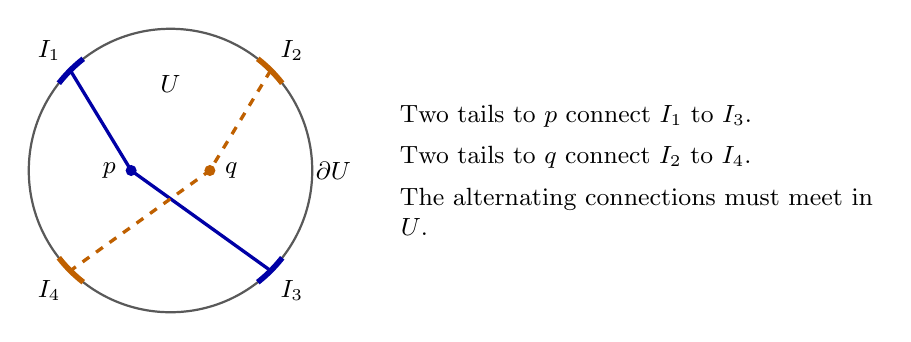
\begin{tikzpicture}[x=1cm,y=1cm,font=\small]
 \draw[black!65,line width=.8pt] (0,0) circle (1.8);
 \draw[blue!65!black,line width=2pt]
 (128:1.8) arc[start angle=128,end angle=142,radius=1.8];
 \draw[orange!75!black,line width=2pt]
 (38:1.8) arc[start angle=38,end angle=52,radius=1.8];
 \draw[blue!65!black,line width=2pt]
 (308:1.8) arc[start angle=308,end angle=322,radius=1.8];
 \draw[orange!75!black,line width=2pt]
 (218:1.8) arc[start angle=218,end angle=232,radius=1.8];
 \node at (2.07,0) {$\partial U$};
 \node at (0,1.1) {$U$};
 \draw[blue!65!black,line width=1.2pt]
 (-1.273,1.273)--(-.5,0)--(1.273,-1.273);
 \draw[orange!75!black,line width=1.2pt,dashed]
 (1.273,1.273)--(.5,0)--(-1.273,-1.273);
 \fill[blue!65!black] (-.5,0) circle (2pt);
 \fill[orange!75!black] (.5,0) circle (2pt);
 \node[left,xshift=-2pt] at (-.5,0) {$p$};
 \node[right,xshift=2pt] at (.5,0) {$q$};
 \node[above left] at (-1.273,1.273) {$I_1$};
 \node[above right] at (1.273,1.273) {$I_2$};
 \node[below right] at (1.273,-1.273) {$I_3$};
 \node[below left] at (-1.273,-1.273) {$I_4$};
 \node[align=left,text width=6cm,anchor=west] at (2.8,0)
 {Two tails to $p$ connect $I_1$ to $I_3$.\\[4pt]
  Two tails to $q$ connect $I_2$ to $I_4$.\\[4pt]
  The alternating connections must meet in $U$.};
\end{tikzpicture}
\caption{The four-path crossing in the quotient disk $U$.
The four boundary arcs occur in cyclic order. After diffuse dust
contacts have been removed, the probability of any required meeting
is bounded by the occupation and hit estimates.}
\label{fig:crossing}
\end{figure}


\smallskip\noindent\emph{Dust intersections.}
We estimate the probability of such a cross-pair intersection.
Lemma~\ref{lem:diffuse-intersections} removes all dust meetings outside
a countable set.  Points in that set with zero hit probability for
either law can also be discarded.  Independence and the union bound
therefore give
\begin{align}
 \label{eq:dust-meeting-bound}
 \Prob(\text{a common visit in }U\cap B)
 &\le \sum_{s\in U\cap B}m_{\mu_p}(s)m_{\mu_q}(s)\notag\\
 &\le m_{\mu_q}(p)+m_{\mu_p}(q)
    +\sum_{s\in(U\cap B)\setminus\{p,q\}}
       m_{\mu_p}(s)m_{\mu_q}(s)\notag\\
 &\le 2\delta+\delta^2.
\end{align}
Here the target hit probabilities equal one, $p\ne q$, and the last
sum is estimated by Cauchy--Schwarz using
Equation~\eqref{eq:small-law-tail}.

\smallskip\noindent\emph{Domain intersections.}
For domain meetings, let $\ell_\gamma$ denote a sample's arclength
occupation restricted to $U\cap G$, and put
\[
 I_a(\gamma,\widetilde\gamma)
 =\iint \frac{\ind_{\{\dist_{\rm sph}(x,y)<2a\}}}{a^2}
       \,\dd\ell_\gamma(x)\,\dd\ell_{\widetilde\gamma}(y).
\]
If the two paths meet at $x\in U\cap G$, then for every sufficiently
small $a$ the physical ball of radius $a$ about $x$ is contained in
$U\cap G$.  Each path has at least $a/2$ of arclength in its ball of
radius $a/2$: after visiting $x$ it must eventually leave the ball in
order to reach its dust endpoint.  Therefore
\[
 \liminf_{a\downarrow0}I_a(\gamma,\widetilde\gamma)\ge\frac14
\]
on the domain-intersection event.  The spherical kernel in this
integral has uniformly bounded integrals in each variable, since
spherical balls of radius $2a$ have area at most a numerical constant
times $a^2$.  Its operator norm on $L^2(\dd a)$ is consequently bounded
by a numerical constant $C$.  Independence yields
\[
 \E I_a
 \le C\|g_{\mu_p}\|_{2,U\cap G}
       \|g_{\mu_q}\|_{2,U\cap G}
 \le C\delta^2.
\]
Applying Fatou's lemma along any sequence $a\downarrow0$ gives
\begin{equation}
 \label{eq:domain-meeting-bound}
 \Prob(\text{a common visit in }U\cap G)\le4C\delta^2.
\end{equation}
The estimates concern the original paths, and hence also bound
intersections of their last-hit tails.

\smallskip\noindent\emph{The contradiction.}
Combining Equations~\eqref{eq:dust-meeting-bound} and
\eqref{eq:domain-meeting-bound}, and taking the union bound over the
four cross-pairs, bounds the alternation event by
\[
 4\bigl(2\delta+(1+4C)\delta^2\bigr).
\]
For sufficiently small $\delta$ this is less than $10^{-4}$, the
contradiction.
\end{proof}

\subsection{Selecting barriers and collapsing unmarked components}

The preceding theorem concerns availability for a fixed prior list.
We use it after a maximal countable selection, so that every point still
uncovered is unavailable for the final list.  Transfinite arguments
also occur in He and Schramm's treatment of countably connected
domains, where the induction follows the Cantor--Bendixson complexity
of the boundary-component space
\cite[p.~373 and Theorem~7.1]{HeSchramm1993}.  Here each new test
enlarges an open set of ends already supplied with a barrier, and
second countability limits the number of strict enlargements.
The whole space of complementary components need not be countable.

Start with an arbitrary countable well-ordered compatible list
$\mathscr L_0$ and its countable flag set $\Sigma_0$.  Append
ungated real barriers for the anchor in
Theorem~\ref{thm:countable-exceptions}, without changing the earlier
coordinates, masks, periods, or budgets.  The seed list may be empty.
During the selection,
let $V_k$ be the relatively open subset of $B$ covered by the inner dust
disks of the newly chosen barriers with norm bound strictly less than
$1/k$, for each $k\in\N$.  At a countable stage, if some pair $(k,b)$
with $b\notin V_k$ admits a compatible barrier with that bound, append
one such barrier and enlarge the flags as permitted.  Its inner dust
disk strictly enlarges $V_k$.
At countable limit stages take unions of the lists and of the flags.
Compatibility persists by its finite-sublist formulation.

This process stops at a countable stage.  Indeed, fix a countable basis
for $B$.  At a step enlarging $V_k$, choose a basis element containing
the previously uncovered endpoint and contained in the new inner dust
disk.  It is now contained in $V_k$ and was not contained in $V_k$
before this step.  The pair consisting of $k$ and this basis element
can never be chosen again.  An $\omega_1$-long sequence of steps would
therefore inject into a countable set, which is impossible.

Let $\mathscr L$ be the resulting countable compatible list and set
\begin{equation}
 \label{eq:first-exceptional-set}
 S=\bigcup_{k\in\N}(B\setminus V_k).
\end{equation}
At termination no endpoint in $B\setminus V_k$ admits an extension
with bound less than $1/k$ for the final list and its final flags.
Theorem~\ref{thm:countable-exceptions}, applied separately for each $k$,
shows that $S$ is countable.  We henceforth include all its points among
the mandatory marks in the finite transfers.

It remains to convert the selected barriers into a statement about
limiting components.  The following estimate pays for a change from zero
to one along a line by the domain gradient and the oscillations across
the round holes it meets.

\begin{lemma}[Payment along parallel lines]
\label{lem:line-payment}
Let $D$ be a finite circle domain containing infinity, with all its
bounded complementary disks contained in $\{|w|<L\}$.  Write their
radii as $r_T$, allowing radius zero.  Let $v$ be a smooth real function
on $D$ of finite energy.  Suppose its cluster values near each
complementary disk lie in a bounded real interval of length at most
$A(T)$.

Fix a direction and a measurable set $J$ of transverse parameters.
Suppose that on each line with parameter in $J$ there is a segment in
$\{|w|\le L\}$ with endpoints in $D$ on which $v$ has values zero and
one.  Then
\begin{equation}
 \label{eq:line-payment}
 |J|\le\sqrt{\pi}\,L\|\dd v\|_{2,D\cap\{|w|\le L\}}
       +2\sum_T r_T A(T)
 \le\sqrt{\pi}\,L\|\dd v\|_2
       +2L\Bigl(\sum_T A(T)^2\Bigr)^{1/2}.
\end{equation}
The same first inequality holds with the gradient integrated over any
measurable region containing all the chosen domain portions of the
segments.
\end{lemma}

\begin{proof}
Discard the finitely many tangent lines and lines through point holes.
For almost every remaining line the gradient integral in the bounded
region is finite.  The intersection of a chosen segment with $D$ is a
finite union of intervals.  On each, ordinary variation bounds the
change of $v$ by the gradient line integral.  Approach the endpoints of
the complementary intervals from within $D$.  The difference across
each such interval is at most $A(T)$, by the cluster-interval
hypothesis.  Equivalently one can first use compact subintervals in
$D$ and then take endpoint limits; finite line variation supplies the
limits whenever needed.  Thus
\[
 1\le
 \int_{D\cap\text{segment}}|\dd v|\,|\dd w|
 +\sum_{T:\,T\cap\text{segment}\ne\varnothing}A(T).
\]
Majorizing by the full-line gradient integral in the radius-$L$ ball
and by all disk hits makes this bound independent of any choice of
segments.  Integration in the transverse parameter and Cauchy--Schwarz
give the first inequality in Equation~\eqref{eq:line-payment}.  A round
disk of radius $r_T$ is met by a set of parallel lines of parameter
length $2r_T$.  Finally the interiors of the disks are disjoint and
lie in the radius-$L$ ball, so
\[
 \sum_T r_T^2\le L^2,
 \qquad
 \sum_T r_T A(T)
 \le L\Bigl(\sum_T A(T)^2\Bigr)^{1/2}.
\]
The proof uses the gradient only on the actual domain portions of the
segments, which also proves the localized assertion.
\end{proof}

\begin{theorem}[Collapse outside the first exceptional set]
\label{thm:unmarked-collapse}
Let $\mathscr L$ and $S$ be obtained by the preceding selection,
starting with any countable compatible seed list.  Extend $\mathscr L$ by any
further countable compatible list, allowing further countable flag
enlargements, and take a diagonal finite-transfer limit $f$ as in
Section~\ref{sec:transfer}.  Then $K_b(f)$ is a singleton for every
$b\in B\setminus S$.
\end{theorem}

\begin{proof}
Fix $b\notin S$.  If $K_b(f)$ had a projection of positive length,
every selected barrier surrounding $b$ would have to pay for that same
length.  Their arbitrarily small norms will contradict this requirement.

Suppose $K_b(f)$ is nondegenerate.  Some orthogonal projection of this
compact continuum has positive length.  Fix a compact interval $J$ of
positive length inside that projection.  The target bound $L$ from
Section~\ref{sec:transfer} can be increased once to contain all images
of the outer zero circle $E_*$ as well as all relevant inner curves and
complementary disks.  This choice is independent of the barrier: the
inner curves lie in the bounded side of the fixed outer curve, whose
image is uniformly bounded.

For each $k$ choose a selected barrier $u$ with
\[
 \|\dd u\|_2+\|a_u\|_{\ell^2}<1/k
\]
whose inner dust disk contains $b$.  Its inner boundary curve $C$ has
value one, and $E_*$ has value zero.  The end-component description
in Lemma~\ref{lem:end-components} places $K_b(f)$ strictly inside the
bounded Jordan region of $f(C)$, which in turn lies inside that of
$f(E_*)$.  For this fixed test, local uniform convergence on the two
curves and stability of winding imply the same inclusions of the fixed
compact set $K_b(f)$ for all sufficiently large finite maps $f_n$.

Each line with parameter in $J$ therefore meets the inner bounded
region.  Following it out toward infinity supplies a segment between
$f_n(C)$ and $f_n(E_*)$, with test values one and zero.  Both endpoints,
and hence the segment, lie in the radius-$L$ ball.  Apply
Lemma~\ref{lem:line-payment} to the transferred test on the finite
target circle domain.  Its energy norm has upper limit at most
$\|\dd u\|_2$, since it agrees with $u$ on exhausting cores and its
remaining energy tends to zero.  Its boundary oscillations satisfy
\[
 A_n(T)\le a_u(s_T)+e_n(T),
 \qquad e_n(T)\ge0,
 \qquad \sum_Te_n(T)^2\longrightarrow0.
\]
The terminal indices $s_T$ are distinct.  Consequently
\[
 \limsup_n\Bigl(\sum_T A_n(T)^2\Bigr)^{1/2}
 \le\|a_u\|_{\ell^2(B)}.
\]
Taking the limit in Equation~\eqref{eq:line-payment} gives
\[
 |J|\le\sqrt{\pi}\,L\|\dd u\|_2+2L\|a_u\|_{\ell^2}
 \le \frac{(\sqrt{\pi}+2)L}{k}.
\]
The interval $J$ is fixed and $k$ is arbitrary, a contradiction.
Further list extensions preserve both the old tests and their
compatibility, so the argument applies to every stated extension.
\end{proof}

\subsection{Free contacts with prior levels}

The first selection has now reduced the component problem to the
countable set $S$.  To construct period coordinates at those ends, we
need a further property of the path laws.  The residual level constraint
already controls residual dust contacts; the next lemma extends that
control to contacts inside tags and obtains a finite expected count of
all intersections with a generic prior level union.

\begin{lemma}[Generic level intersections of a path law]
\label{lem:law-levels}
Fix a countable prior compatible list with flag set $\Sigma$, possibly
containing period coordinates, and let $\mu$ be a law from
Theorem~\ref{thm:positive-law}.  For every prior coordinate $i$, almost
surely the trace values modulo one at the free points of the path in
$B\cap M_i$ form a Lebesgue-null subset of $\T$.

Consequently, for almost every tuple defining any fixed finite prior
level union $H$,
\[
 \Prob_\mu\{\gamma([0,1])\cap H\cap(B\setminus\Sigma)
                         =\varnothing\}=1,
 \qquad
 \E_\mu\#\bigl(\gamma([0,1])\cap H\bigr)<\infty.
\]
For one coordinate the integrated distinct-intersection bound is
\begin{equation}
 \label{eq:law-level-count}
 \int_\T\E_\mu\#\bigl(\gamma([0,1])\cap H_i(t)\bigr)\,\dd t
 \le \int_{G\cap M_i}g_\mu|\dd u_i|\,\dd a
       +\sum_{s\in B}m_\mu(s)a_i(s)<\infty.
\end{equation}
\end{lemma}

\begin{proof}
We first show that, at a generic independent level, free contacts inside
a tag can occur only in singleton level components.  A detour around
such singleton contacts then gives a variation estimate for the prior
coordinate along the tag.  That estimate makes the free trace image
null.  Finally, coarea counts the remaining intersections.

\emph{Singleton contacts at an independent level.}
Fix a tag slot, its type, and a prior coordinate $i$.  For almost every
pair consisting of the tag tuple and an independent level $t$, every
free contact of that tag with $H_i(t)$ has a singleton component in
$H_i(t)$.  To prove this, exclude equality between $t$ and every level
of label $i$ in the tag, and impose the finitely many relevant
instances of \textup{(P)}.  If a level of some tag label $j>i$ is present
at a contact $x$, \textup{(P)} for $j$ against $i$ gives the assertion.
If no such higher label is present, the tag yields a nondegenerate
local continuum through $x$ in labels lower than $i$, exactly as in
the proof of Lemma~\ref{lem:diffuse-intersections}.  This is forbidden
by \textup{(P)} for $i$.  Closedness permits levels absent at $x$ to
be removed locally.  Absolute continuity of the tuple law in each slot
and type, followed by Fubini, shows that for almost every sample this singleton
assertion holds for almost every $t$, simultaneously for all its tags.

\emph{A local variation bound.}
Near a free point in $B\cap M_i$, choose an open topological disk
$V$ contained in the interior of the mask, away from the singularity
if there is one.  For a period coordinate choose a common lift on
$V$.  Shrink $V$ until all the defined values and bands of this
branch lie in one real interval of length less than $1/2$.  Such a
choice is possible because the point has a unique trace.  A countable
family of these disks covers the relevant free points.

Consider two free contact times $r<s$ in one tag such that
$\gamma([r,s])\subset V$.  Let their real trace values be $\alpha$
and $\beta$.  We claim that
\begin{equation}
 \label{eq:tag-trace-variation}
 |\beta-\alpha|\le
 \int_{[r,s]\cap\gamma^{-1}(G\cap M_i)}|\dd u_i|(\gamma)\,\dd s
 +\sum_{\substack{t\in[r,s]\colon\gamma(t)\in\Sigma\cap M_i}}
      a_i(\gamma(t)).
\end{equation}
Here the sum again counts parameter times.  Assume $\alpha<\beta$.
For almost every real threshold $v\in(\alpha,\beta)$ the preceding
singleton assertion holds at its modulo-one level.  We show that the
segment must hit this threshold either at a domain point or in a
flagged band.

Otherwise the compact set
\[
 F_v=\gamma([r,s])\cap H_i(v\bmod1)
\]
consists only of free points that are singleton components of the
closed level.  They remain singleton components after adjoining $B$,
by the dust topology of Section~\ref{sec:setup}.  The small-disk
construction of Lemma~\ref{lem:dust-disks} covers $F_v$ by finitely
many open disks with closures in $V$, missing the endpoints and with
boundaries avoiding the entire closed level and $B$.  Process these
disks successively on the current path segment, skipping any whose
interior is no longer met.  Replace the portion from first entry to
last exit of a disk by an arc of its boundary.  Each replacement
removes the current level hits in that disk and adds none, so after
the finite process all level hits have disappeared.  Disks need not
be disjoint for this argument.

The resulting path in $V$ cannot exist.  Off the level, the sign of
the chosen branch relative to $v$ is defined at domain points and at
dust points by their bands, and is locally constant.  At dust points
this follows from the defining upper and lower limits of the band.
The endpoint signs are opposite.  The local range of length less
than $1/2$ ensures that no other integer translate of the level is
involved.  This proves the required domain-or-flag hit for almost
every intervening threshold.

The set of values contributed by the domain times has length at most
the integral in Equation~\eqref{eq:tag-trace-variation}: exhaust the
countably many domain intervals and apply ordinary curve variation
on their rectifiable physical portions.  The flagged bands contribute
at most the sum in that equation.  These ranges cover almost every
threshold between $\alpha$ and $\beta$, proving the claim.  The case
$\beta<\alpha$ follows by reversing the endpoints.

\emph{Null trace image.}
For almost every sample, the right-hand costs above are the
restrictions of a finite measure $\kappa_i$ on path time: its domain
part is $|\dd u_i|\,\dd s$ within the mask, and it has an atom of mass
$a_i(\gamma(t))$ at each flagged visit time.  Indeed
\[
 \E_\mu\kappa_i([0,1])
 \le \|g_\mu\|_2\|\dd u_i\|_{2,G\cap M_i}
      +\|n_\mu|_\Sigma\|_{\ell^2}\|a_i\|_{\ell^2}<\infty.
\]
The measure gives zero mass to free contact times.  Fix a tag and one
of the disks $V$.  By outer regularity, its free contact times in
$\gamma^{-1}(V)$ have an open cover, within that tag and
$\gamma^{-1}(V)$, of arbitrarily small $\kappa_i$-measure.  The cover
has countably many interval components.  Within each component,
Equation~\eqref{eq:tag-trace-variation} bounds the diameter of the
free trace image by the measure of that component.  Summing proves
that the free trace image in this tag and this disk has length zero.
The disks and tags are countable.

On residual times, the same null-image conclusion follows directly
from the residual level constraint by deleting the flags, as in the
proof of Lemma~\ref{lem:diffuse-intersections}.  Thus all free contacts
have null trace image.  Singular points are flagged and play no role
in this assertion.

\emph{Distinct intersection counts.}
The image of the domain times is countably rectifiable, and its
physical length measure is dominated by the arclength occupation.
The one-dimensional area formula applied to the smooth map $u_i$
modulo one, in local physical charts and lifts, bounds the integrated
number of distinct domain intersections by
\[
 \int_{G\cap M_i}g_\mu|\dd u_i|\,\dd a.
\]
This also applies at mask boundaries by local smoothness; the
occupation of each such fixed smooth boundary is zero almost surely
because its area is zero.  At a dust point, the parameter length of
level incidence is at most $a_i(s)$.  The already proved null-image
assertion removes free incidences under the joint law and level
measure.  On the countable flags, Tonelli gives the remaining bound
$\sum_s m_\mu(s)a_i(s)$, including a possible singular point with its
budget one.  Cauchy--Schwarz makes both bounds finite and proves
Equation~\eqref{eq:law-level-count}.

For a finite union, sum these bounds over its finitely many labels
and apply Fubini to its level tuple.  The null free-incidence assertion
also passes to that union.  Incidence and distinct finite-point counts
are measurable in the completed sense supplied by the path coding,
so these integrations are legitimate.
\end{proof}

\section{Period coordinates and the marked components}\label{sec:streams}

The first selection has made every unmarked complementary component a
point.  It remains to show that, at each marked end, the limiting round
disk fills the entire complementary component.  Suppose that part of the
component protrudes beyond that disk.  A sufficiently small real barrier
excludes the protrusion by the line-payment estimate.  If no such barrier
exists, an endpoint law produces a coordinate with additive period one.
Before smoothing, its boundary variation is a probability measure; its
energy and its oscillations at all other ends can be made arbitrarily
small.  These properties give incompatible lower and upper bounds for a
boundary integral, the upper bound coming from Stokes' theorem.

Throughout this section the prior coordinate list is an arbitrary
countable list satisfying (P).  All references to free points use its
current flag set, enlarged when a new coordinate is appended.

\subsection{Reduction to a compact family of simple arcs}

We first retain only the terminal portions of the endpoint paths and
erase their loops.  Restricting the resulting law to a compact family
will give the uniform winding bounds needed for the period coordinate.

\begin{lemma}[Compact simple-arc reduction]\label{lem:compact-arcs}
Let $\mu$ be an endpoint law supplied by
Theorem~\ref{thm:positive-law}, with target $b$ and prescribed collars
$C_j(b)=\partial U_j(b)$.  For every sufficiently deep prescribed collar
$C=\partial U$, there is a probability law $\eta$ supported on a compact
subset of $C([0,1],X)$ consisting of simple arcs $\alpha$ such that
\[
 \alpha(0)\in C,\qquad \alpha(1)=b,\qquad
 \alpha((0,1))\subset U\setminus\{b\}.
\]
Its mean domain occupation has a density $g_\eta$ satisfying
\begin{equation}\label{eq:arc-occupation}
 g_\eta\le 2\ind_{U\cap G}g_\mu
 \quad\text{almost everywhere},
 \qquad
 m_\eta(s)\le 2m_\mu(s)\quad(s\in B\cap\overline U),
\end{equation}
and $m_\eta=0$ outside $\overline U$.  Here $m$ denotes hit
probabilities, rather than visit counts.  In particular, for every
$\eps>0$, every sufficiently deep prescribed collar admits such a law
$\eta$ with
\begin{equation}\label{eq:arc-smallness}
 \|g_\eta\|_2+
 \|m_\eta|_{B\setminus\{b\}}\|_{\ell^2}
 <\eps.
\end{equation}

For almost every tuple defining any fixed finite prior level union $H$,
the expected number of distinct intersections of an arc with $H$ is
finite, and the arcs almost surely have no free dust contacts in $H$.
If the endpoint problem has gates, the starting point additionally
satisfies $f_0(\alpha(0))\in\overline W_2$.
\end{lemma}

\begin{proof}
Cut each path at its last hit of $C$ and retain its terminal part,
reparametrized on $[0,1]$.
The anchor is outside $\overline U$, so such a hit exists.  Its last
hitting time is strictly less than $1$; after that time the path is
strictly inside $U$.  The original path reaches $b$ for the first time
at its endpoint.  Thus its terminal part has distinct endpoints and
contains a simple arc with those endpoints.  The gate condition passes
to the last hitting point.

These operations can be performed measurably up to completion of the
law.  Last hitting times of a fixed closed set are Borel on the present
path family.  In the product of two path spaces, the conditions that
the second path is injective, has prescribed endpoints, and has image
contained in the first path's image are Borel.  For injectivity, use
\[
 \min_{|s-t|\ge 1/n}d_X(\alpha(s),\alpha(t))>0
 \qquad(n\in\N);
\]
image containment is closed for uniform convergence.  The nonempty
sections therefore admit a universally measurable selection by the
Jankov--von Neumann theorem \cite[Theorems~18.1 and 29.9]{Kechris1995}.  The
pushforward of the completed probability measure is an ordinary Borel
probability measure on path space.

The occupation measure of a selected simple arc is its domain image
length measure.  By the image-length observation in
Section~\ref{sec:barriers}, this is dominated by the occupation of the
original terminal path.  There is no arclength atom at its initial
point on $C$.  Consequently the unconditioned selected-arc law has
occupation density at most $\ind_{U\cap G}g_\mu$, and its hit probabilities are
at most the original hit probabilities.  The endpoint and interior
conditions describe a Borel subset of path space.  Inner regularity
provides a compact subset of that set of probability at least $1/2$.
Conditioning on this subset proves Equation~\eqref{eq:arc-occupation}.

The indicators of $U_j(b)\cap G$ decrease pointwise to zero.  The
square-summable function $m_\mu$ has countable support, and the sets
$(U_j(b)\cap B)\setminus\{b\}$ decrease to the empty set.  Absolute
continuity of the two squared integrals therefore proves
Equation~\eqref{eq:arc-smallness}.  Finally, all selected images are
subsets of the original images.  The level-intersection conclusions of
Lemma~\ref{lem:law-levels} survive restriction, selection, and
conditioning, with their expected counts increased by at most the
conditioning factor.
\end{proof}

\subsection{Averaging the index of a ray}

Each simple arc will determine an integer-valued function on the cyclic
cover of the punctured dust disk.  We average these functions to obtain
a continuous period coordinate, then smooth it while preserving all
nonsingular bands.

\begin{lemma}[A stream coordinate]\label{lem:stream}
Let $U$ be a dust disk, let $b\in B\cap U$, and put $C=\partial U$.
Suppose $\eta$ is supported on a compact family of simple arcs from $C$
to $b$, meeting $C$ only at their initial points and $b$ only at their
terminal points.  Assume that its mean domain occupation has an
$L^2$ density $g_\eta$, that $m_\eta\in\ell^2(B)$, and that it has
the generic level-intersection conclusions of
Lemma~\ref{lem:compact-arcs} for the prior list.

There is a continuous, locally Sobolev function $v$ on the cyclic cover
over $G\cap\overline U$, with additive period one about $b$, such that
\begin{equation}\label{eq:stream-energy}
 \|\dd v\|_{2,G\cap U}\le\sqrt2\,\|g_\eta\|_2.
\end{equation}
At every $s\in B\cap U\setminus\{b\}$ its band is bounded and has
width at most $m_\eta(s)$.  After enlarging the flags by
$\{s\in B:m_\eta(s)>0\}$, its free traces satisfy (P) against the
prior list.
If $\beta$ is the probability distribution of the arc starts on the
positively oriented curve $C$, then $\beta$ is atomless and
\begin{equation}\label{eq:stream-boundary-measure}
 \dd(v|_C)=\beta.
\end{equation}
This equality is understood on a lifted boundary interval: the branch
increases by one over a full turn.

For every $\eps>0$ one may replace $v$ by a smooth coordinate $u$ of
the same period such that
\begin{equation}\label{eq:stream-smoothing}
 \|\dd(u-v)\|_{2,G\cap U}<\eps,
 \qquad \sup_C|u-v|<\eps,
\end{equation}
with the same nonsingular bands and hence with (P).  The discrepancy
$u-v$ is single-valued.  Thus $u$ is an admissible coordinate with
mask $\overline U$ and budget
\[
 a_u(s)=m_\eta(s)\quad(s\in B\cap U\setminus\{b\}),
 \qquad a_u(b)=1,
\]
and zero budget off its mask.
\end{lemma}

\begin{proof}
We first construct $v$ and prove its energy estimate and boundary-measure
identity.  We then control its dust bands and free traces, and finally
produce the smooth admissible coordinate $u$.

\smallskip\noindent\emph{Step 1: the lifted rays.}
Choose an orientation-preserving homeomorphism from
$(\overline U,b)$ to the closed unit disk with its center.  Write the
cyclic cover of $\overline U\setminus\{b\}$ as
\[
 \mathcal H=\R\times[0,\infty),
\]
where the first coordinate is angle divided by $2\pi$, the second is
minus logarithmic radius, and the deck transformation is
$(x,y)\mapsto(x+1,y)$.  These are topological coordinates; all analytic
estimates below will instead use physical conformal charts in $G$.

For an arc $\alpha$, choose the lift starting at $(a,0)$ with
$a\in[0,1)$.  Its image $\Gamma_\alpha$ is a proper simple ray with
$y\to\infty$ at its terminal end.  Its integer translates are disjoint:
an intersection of two translates would give a repeated projected
point of the simple arc.  In the one-point compactification of
$\mathcal H$, the translated ray $\Gamma_\alpha+(k,0)$ is a crosscut
from $(a+k,0)$ to the boundary point at infinity.  Let $R_k(\alpha)$
be its right-hand complementary component, the one incident to boundary
points $(x,0)$ with $x>a+k$.
Jordan separation gives
\[
 R_{k+1}(\alpha)\subset R_k(\alpha).
\]
Indeed the next ray lies on the right of the preceding ray because it
is connected, is disjoint from that ray, and starts on its right.
The right side of the next ray connects to boundary points right of
both starts and is therefore contained in the preceding right side.

\smallskip\noindent\emph{Step 2: the integer index and its local bounds.}
Compactness of the arc family has two consequences.  The arcs approach
$b$ uniformly as the parameter tends to $1$; and, for every
$\delta>0$, their portions with parameter in $[0,1-\delta]$ stay a
uniform positive distance from $b$.  The first assertion follows from
equicontinuity and the common terminal endpoint.  The second follows
from compactness and the fact that every member is injective and meets
$b$ only at parameter $1$.

Fix $0\le Y<\infty$.  Uniform approach to $b$ gives $\delta>0$ such that
every arc point with $0\le y\le Y$ occurs before the common time
$1-\delta$.  On this initial interval the arcs stay uniformly away
from $b$, so their projected circular positions are equicontinuous.
Subdivide time into finitely many intervals on each of which all circular positions
move by less than a semicircle.  Starting with $a\in[0,1)$, successive
lifts then give a uniform bound for all lifted angles on this initial
interval.  Thus all unshifted rays in the strip $0\le y\le Y$ lie
in a common bounded horizontal interval.

For a compact subset of $\mathcal H$, join its points vertically to
the boundary.  Sufficiently large positive or negative translates
miss all those vertical segments.  Their side at the boundary is
fixed by the order of the starts, and it remains fixed along the
segments.  Hence, for every $z$ off the translated rays, the set
$\{k\in\Z:z\in R_k(\alpha)\}$ is nonempty and bounded above.  We may
therefore define
\begin{equation}\label{eq:ray-index}
 J_\alpha(z)=\max\{k\in\Z:z\in R_k(\alpha)\}.
\end{equation}
The same argument bounds $|J_\alpha|$ uniformly over the arc family
on each compact subset of $\mathcal H$, wherever it is defined.
The definition also gives
\begin{equation}\label{eq:ray-index-period}
 J_\alpha(z+(1,0))=J_\alpha(z)+1,
 \qquad J_\alpha(x,0)=\lfloor x-a\rfloor
 \quad(x-a\notin\Z).
\end{equation}

\smallskip\noindent\emph{Step 3: measurability and an intersection inequality.}
The lifted arc on every initial compact time interval is a Borel
function of the arc and its chosen starting angle, by path lifting.
Off a ray, membership in its right component is Borel as well.  One
may test it by countable chains of rational open balls disjoint from
the ray and joining the point to the appropriate boundary interval.
Avoidance of a compact test path is Borel by the initial lifts and a
countable exhaustion of $[0,1)$.  Since a compact path disjoint from a
closed proper ray has positive distance from it, these tests detect
all complement connections.  This proves measurability of the
indices.  On the coincidence set, where $z$ lies on a translated ray,
assign an arbitrary value whenever a random variable is required.  We
will take expectations only at points whose coincidence probability is
zero.

Suppose a curve $\delta$ in the cover projects injectively to
$\overline U\setminus\{b\}$ and its endpoints miss the sample rays.
Every ray separating the endpoint indices must meet $\delta$.
Different such meetings project to different points because the
projection of $\delta$ is injective.  Consequently
\begin{equation}\label{eq:index-intersections}
 |J_\alpha(\delta(1))-J_\alpha(\delta(0))|
 \le \#\bigl(\alpha([0,1])\cap\operatorname{proj}\delta([0,1])\bigr).
\end{equation}
The right side counts distinct projected points; the inequality also
holds when that count is infinite.

\smallskip\noindent\emph{Step 4: averaging and continuity.}
The index is now defined, measurable, and locally uniformly bounded.
We use these properties to average it.
Lemma~\ref{lem:point-avoidance} applies to $\eta$, since its arcs
end at $b\in B$ and have an $L^2$ mean occupation density.
Thus every fixed point of $G\cap\overline U$, including a point
of $C$, is missed almost surely.  For each lift $z$ of such a point,
define
\[
 v(z)=\E_\eta J_\alpha(z).
\]
Local uniform domination makes this expectation finite.  For a
convergent sequence in the lifted domain, discard the null coincidence
events at its terms and its limit.  For every remaining sample the
index is locally constant at the limit.  Dominated convergence proves
continuity of $v$, including at $C$.  The first identity in
Equation~\eqref{eq:ray-index-period} gives additive period one.

\smallskip\noindent\emph{Step 5: the differential estimate.}
Work in a physical conformal rectangle compactly contained in $G\cap U$,
with a common lift.  Here $z=x+iy$ denotes a physical conformal
coordinate, and the spherical metric is $\lambda(z)|\dd z|$; these
$x,y$ are unrelated to the topological angle and depth above.
For a horizontal interval $I$ and height $y$ let
$N_\alpha(I,y)$ count the distinct intersections of the sample arc
with $I\times\{y\}$.  Curve coarea, followed by the occupation bound,
gives, for Borel sets $A$ of heights,
\begin{equation}\label{eq:stream-slice-coarea}
 \int_A\E_\eta N_\alpha(I,y)\,\dd y
 \le \int_{I\times A}\lambda(z)g_\eta(z)\,\dd x\,\dd y.
\end{equation}
To check the conformal factor, Euclidean image length is spherical
image length divided by $\lambda$, whereas spherical area is
$\lambda^2\dd x\dd y$.  Projection coarea costs at most Euclidean
image length.  The same estimate holds after restricting counts to
Borel portions of an interval.

Apply Equation~\eqref{eq:stream-slice-coarea} first to closed intervals
with rational endpoints.  Outside one null set of heights, the mean
counting measure on every compact interior interval is bounded by
$\lambda g_\eta\dd x$.  This follows by the countable interval tests
and then measure approximation.  Averaging
Equation~\eqref{eq:index-intersections} shows on those lines that
\[
 |v(x_2,y)-v(x_1,y)|
 \le\int_{x_1}^{x_2}\lambda(x,y)g_\eta(x,y)\,\dd x.
\]
Continuity permits arbitrary endpoints.  Thus $v$ is absolutely
continuous on almost every horizontal line and
$|\partial_xv|\le\lambda g_\eta$ there.  The vertical argument gives
$|\partial_yv|\le\lambda g_\eta$.  The usual characterization by
absolute continuity on lines yields local Sobolev regularity and
\[
 |\dd v|_{\mathrm{sph}}\le\sqrt2\,g_\eta
 \quad\text{almost everywhere}.
\]
An exhaustion by charts proves Equation~\eqref{eq:stream-energy}.

\smallskip\noindent\emph{Step 6: the boundary measure.}
The distribution $\beta$ of the starting point has no atoms by point
avoidance on $C$.  Between two ordered lifted boundary angles, the
expected difference of the floors in
Equation~\eqref{eq:ray-index-period} counts the mean number of start
translates in that interval.  This proves
Equation~\eqref{eq:stream-boundary-measure}.  In particular, for every
continuous real function $\varphi$ on $C$,
\begin{equation}\label{eq:stream-boundary-integral}
 \int_C\varphi\,\dd v
   =\int\varphi(\alpha(0))\,\dd\eta(\alpha).
\end{equation}
The left side is a Stieltjes integral.  Only the orientation of the
topological angular coordinate is used; no smoothness is required.

We have obtained a continuous period coordinate with the required
energy bound and a positive boundary measure of total mass one.  To
make it admissible for transfer, we must still control its dust bands,
verify compatibility, and smooth it.

\smallskip\noindent\emph{Step 7: bands at the dust.}
Fix $s\in B\cap U\setminus\{b\}$ and a lift of a neighborhood of
$s$.  Consider two sequences of domain points tending to that lift.
At all terms of both sequences the sample index is defined almost
surely. For each sample, Step~2 shows that only finitely many translated
rays meet a compact neighborhood of the chosen lift. Shrink to a connected
neighborhood missing those rays that do not pass through the lift; their
side memberships are then fixed. If the projected sample misses $s$,
the eventual index difference is therefore zero. Otherwise simplicity
leaves just one ray through the lift. Only membership in its right-hand
component can vary, so the index has at most two adjacent values. Hence
the upper limit of the absolute index difference is at most one.
The local uniform bound and the reverse Fatou inequality now give
\[
 \limsup |v(z_n)-v(w_n)|\le m_\eta(s).
\]
Local boundedness makes the upper and lower bands finite, and choosing
sequences approaching their extremes proves the asserted width bound.
When $m_\eta(s)=0$, the unique trace is $\E_\eta J_\alpha(s)$.

\smallskip\noindent\emph{Step 8: compatibility.}
Put $\Sigma'=\Sigma\cup\{s\in B:m_\eta(s)>0\}$, a countable
enlargement of the flags.  Fix a generic finite prior level union $H$.
By hypothesis the rule
\[
 \nu(A)=\E_\eta\#\bigl(A\cap H\cap\alpha([0,1])\bigr),
 \qquad A\subset H\text{ Borel},
\]
defines a finite measure.  It gives zero mass to
$H\cap(B\setminus\Sigma')$, since almost every sample avoids this
whole set.  The counting integrals are measurable by compact incidence
tests and finite distinct-point tests in path space; finite expected
total count then defines the measure on all Borel subsets.

Let $K$ be a nondegenerate component of $H$ and work in a small disk
$V$ with closure in $U\setminus\{b\}$ and with a common lift.
For free points $x,y\in K\cap V$ joined by a simple arc
$\delta\subset K\cap V$, their traces are expectations of the
indices.  Equation~\eqref{eq:index-intersections} gives
\begin{equation}\label{eq:stream-trace-control}
 |v(x)-v(y)|\le\nu(\delta).
\end{equation}
Set $F=K\cap V\cap(B\setminus\Sigma')$.  We have $\nu(F)=0$,
and $K$ is locally connected by Lemma~\ref{lem:level-continua}.
Equation~\eqref{eq:stream-trace-control} verifies the arc hypothesis
of Lemma~\ref{lem:trace-null} for the continuum $K$, the relatively
open set $K\cap V$, the measure $\nu|_K$, and the free set $F$.
Hence its real trace image has Lebesgue outer measure zero.
Countably many components $K$ and lifted disks $V$ suffice.
The singular point $b$ is flagged.  Fubini in the level parameters
therefore proves (P) for the new coordinate.  All incidence statements
may use completed measures, as in the earlier level arguments.

\smallskip\noindent\emph{Step 9: smoothing.}
It remains to smooth $v$ with an error that vanishes at every dust
point, so that all nonsingular bands remain unchanged.
Near the smooth curve $C$, the continuous Sobolev branches extend
across the boundary by reflection in smooth collar charts.  Cover
$G\cap\overline U$ by a locally finite family of relatively compact
simply lifted patches and take a smooth partition of unity.  Smooth a
branch on each patch; on other sheets use its integer translates.
The local smoothing discrepancy is single-valued, so partition
interpolation respects the additive period.

Choose a continuous positive tolerance $e$ on the source patches with
\[
 0<e(x)\le\tfrac12\min\{\eps,\dist_X(x,B)\},
 \qquad x\in G\cap\overline U.
\]
It extends positively across the compact collar of $C$.  On the $j$th
patch choose the branch approximation error in values smaller than
the positive infimum of $e$ on the corresponding compact partition
support.  Simultaneously make its Sobolev error, including the
derivatives of the partition function, less than $\eps2^{-j}$.
Local continuity and Sobolev approximation permit both requirements.
Partition interpolation then gives $|u-v|(x)\le e(x)$, while the
differential errors are summable.  The resulting $u$ satisfies
Equation~\eqref{eq:stream-smoothing} and is smooth up to $C$.
For every domain sequence tending in $X$ to a nonsingular dust point,
$e(x)$ tends to zero; hence the upper and lower band limits are
exactly unchanged in a common local lift.  Its free traces are
therefore unchanged.  Since compatibility for a newly appended
coordinate concerns only those traces against earlier level unions,
(P) is preserved.
\end{proof}

\subsection{A boundary estimate for a transferred stream}

The boundary-measure identity will provide a lower bound near a
protrusion.  The following Stokes estimate supplies the upper bound in
a finite completion, using the energy and the oscillations at the
other holes.

\begin{lemma}[Stokes estimate]\label{lem:stream-stokes}
Let $u$ be a smooth period coordinate with mask $\overline U$ and
singularity $b$, and put $C=\partial U$.  Transfer it to a finite
completion retaining $C$ and the marked hole indexed by $b$.  Write
$F$ for the normalized circle-domain map, $u^*$ for the transferred
coordinate in the target, and $D_b$ for the distinguished round hole.
Assume that the masked region lies in $|w|<L$.  Target lengths and areas
are Euclidean; the norm below is over the domain inside $F(C)$ and
outside its circular holes.  For a target hole $T$ inside
$F(C)$, let $s_T$ be the index of its source terminal disk and $r_T$
its radius.  When $s_T\ne b$, let $A_u(T)$ be its transferred boundary
oscillation.  Then
\begin{equation}\label{eq:stream-stokes}
 \left|\int_{F(C)}\dist(w,D_b)\,\dd u^*\right|
 \le \sqrt\pi L\,\|\dd u^*\|_2
       +2\pi\sum_{T:\,s_T\ne b}r_TA_u(T).
\end{equation}
Consequently, along diagonal transfers $F_n$ with errors tending to zero,
write $u_n^*$ for the transferred coordinate and $D_{n,b}$ for its
distinguished target disk.  Then
\begin{equation}\label{eq:stream-stokes-asymptotic}
 \limsup_{n\to\infty}
 \left|\int_{F_n(C)}\dist(w,D_{n,b})\,\dd u_n^*\right|
 \le \sqrt\pi L\,\|\dd u\|_{2,G\cap U}
       +2\pi L\,\|a_u|_{B\setminus\{b\}}\|_{\ell^2}.
\end{equation}
\end{lemma}

\begin{proof}
Put $\phi(w)=\dist(w,D_b)$.  Its weak gradient has norm at most one.
Apply Stokes' theorem in the region inside $F(C)$ after replacing each
circular hole by a slightly larger concentric circle.  There are only
finitely many holes, so the offsets can be chosen disjoint and inside
the domain.  The exterior boundary integral is the wedge integral
$\int\dd\phi\wedge\dd u^*$ plus the integrals around the offset
circles, each with positive disk orientation.

On the distinguished offset of radius $r_b+\rho$, $\phi$ is the
constant $\rho$.  The period of $u^*$ there is one, so its contribution
is $\rho$ and tends to zero.

At every other hole the period is zero, so there is a single-valued
branch.  Subtracting a constant from that branch and integrating by
parts bounds the boundary integral by
\[
 2\pi(r_T+\rho)\bigl(A_u(T)+o(1)\bigr).
\]
Here $|\dd\phi|\le|\dd w|$ along the Euclidean offset circle, and
the oscillation on small offsets tends
to at most $A_u(T)$ by the collar correspondence in
Lemma~\ref{lem:end-components}.  This argument also covers a hole of
radius zero.  The remaining region has Euclidean area at most
$\pi L^2$, so Cauchy--Schwarz bounds the wedge integral by
$\sqrt\pi L\|\dd u^*\|_2$.  Letting the offsets
tend to zero proves Equation~\eqref{eq:stream-stokes}.

Disjointness of the disk interiors gives $\sum_T r_T^2\le L^2$.
The terminal indices are distinct, and the index $b$ occurs only at
the distinguished hole.  The positive-excess estimate of
Theorem~\ref{thm:transfer} therefore gives
\[
 \left(\sum_{T:\,s_T\ne b}A_u(T)^2\right)^{1/2}
 \le \|a_u|_{B\setminus\{b\}}\|_{\ell^2}+o(1).
\]
Conformal invariance of Dirichlet energy and the energy estimate of
that theorem also give
$\|\dd u^*\|_2\le\|\dd u\|_{2,G\cap U}+o(1)$.
A second application of Cauchy--Schwarz proves
Equation~\eqref{eq:stream-stokes-asymptotic}.
\end{proof}

\subsection{Excluding a protrusion}

We now apply the barrier alternative and the Stokes estimate to a fixed
normalized map and a round disk properly contained in one of its marked
components.  The estimates will exclude a whole neighborhood of that
pair, allowing the final selection to use only countably many tests.

For a fixed mark $b$, let $\mathcal Q_b$ be the space of pairs $(f,D)$
where $f$ is a normalized univalent map on $G$ and $D$ is a closed
round disk, possibly a singleton, contained in $K_b(f)$.  Give maps
the compact-open topology and disks their center-radius topology,
equivalently the Hausdorff topology on the bounded disks considered
here.  These pair spaces are second countable.  A pair is \emph{bad}
if $D\ne K_b(f)$.

\begin{lemma}[Local exclusion of a bad pair]\label{lem:bad-pair}
Given a countable prior list satisfying (P), a mark $b$, and a bad
pair $(f_0,D_0)\in\mathcal Q_b$, one can append a compatible real
barrier or a compatible period coordinate singular at $b$ such that
an entire relative neighborhood of $(f_0,D_0)$ is excluded as limiting
pair data of diagonal finite transfers.  The exclusion persists after
any further countable extensions satisfying (P), provided $b$ remains
marked.
\end{lemma}

\begin{proof}
We first fix geometry that will serve both alternatives.  In the
barrier case it gives a family of line segments with a fixed positive
transverse width.  In the law case it keeps the arc starts a fixed
positive distance from $D_0$.

\smallskip\noindent\emph{Fixed geometry near the protrusion.}
Write $K=K_b(f_0)$.  There is a boundary point $x$ of $K$ outside
$D_0$: for example, maximize distance to the center of $D_0$ on $K$.
Choose a bounded open ball $W_2$ about $x$ whose closure misses $D_0$,
and a smaller closed ball $W_1$ about $x$ contained in $W_2$.
Boundary bumping, applied in a still smaller closed ball, gives a
nondegenerate subcontinuum $Q\subset K\cap\operatorname{int}W_1$.
The ball can be chosen small enough that $K$ also has points outside
it, because $D_0\subset K$ is separated from $x$.

Every boundary point of a complementary component is approached from
the domain.  Indeed, if a ball about such a point missed the domain,
the connected ball would lie in that same complementary component,
contradicting that the point was a boundary point.  Thus choose a
small closed ball $A\subset f_0(G)\cap\operatorname{int}W_1$ and
nested smaller balls strictly inside $A$.  Their preimages give an
anchor $E$ and a compact testing set
$E_*\subset\operatorname{int}E$.  Start the collar sequence deep
enough that its closed disks miss $E$.

There is a direction and a closed interval $J$ of positive transverse
width such that every line with transverse parameter in $J$ joins a
point strictly inside $f_0(E_*)$ to a point of $Q$, by a segment in
$\operatorname{int}W_1$.  To see this, first direct a line from the
center of the smallest anchor ball to a point of $Q$.  That point
projects strictly inside the ball's transverse projection.  Perturb
the direction, if necessary, so that the transverse projection of
$Q$ is nondegenerate.  The projection is an interval, and it overlaps
the interior of the anchor-ball projection in positive length.  Take
$J$ compactly inside that overlap.  Choose the starts on the middle
chords of the anchor ball; they then have a uniform interior buffer.
Convexity of $W_1$ puts the segments inside it.

These sets and $J$ are fixed before the test's collar and penalty
region are chosen.  For every prescribed collar $C_l$, the compact
continuum
$Q$ lies strictly inside the bounded side of $f_0(C_l)$, whereas the
buffered starts lie outside.  After a collar is fixed these inclusions
persist under sufficiently small changes of the map, by winding
number on $C_l$ and on the boundary of $E_*$.  In particular the
buffered starting points remain images of points in $E_*$.

\smallskip\noindent\emph{The barrier case.}
Use the endpoint problem with these anchors and with gates prescribed
by $(f_0,W_1,W_2)$.  Let $c_L$ be a constant large enough for the
line-payment estimate in the common target size bound.  Fix
$\tau>0$ with $c_L\tau<|J|/2$.
If there is a compatible barrier $u$ with
\[
 \|\dd u\|_{2,G\setminus O}+\|a_u\|_{\ell^2}<\tau,
\]
append it.  It equals zero on $E_*$ and one on some fixed inner
collar $C_l$.  In sufficiently close finite-map data the segments just
constructed start in the zero region and reach the side inside
$F(C_l)$; stop each segment at its first hit of that curve.  The
compact set $\overline O$ has image disjoint from $W_1$ under
$f_0$, and this separation persists under convergence on
$\overline O$.  Thus all gradients paid along these segments lie off
the image of $O$.

Lemma~\ref{lem:line-payment}, with the transfer error tending to zero,
gives
\[
 |J|\le c_L\bigl(\|\dd u\|_{2,G\setminus O}
                          +\|a_u\|_{\ell^2}\bigr)+o(1),
\]
a contradiction to $c_L\tau<|J|/2$.  To justify the restricted
energy estimate, retain $\overline O$ in the unchanged
core and use the original energy off $O$ there, together with the
transfer error on the rest.  All required separations involve fixed
compact sets after $u$, $C_l$, and $O$ have been chosen.  This excludes
a relative neighborhood of $f_0$, and hence a relative neighborhood
of $(f_0,D_0)$.

\smallskip\noindent\emph{The law case.}
If no such barrier is available, Theorem~\ref{thm:positive-law}
provides an endpoint law $\mu$ obeying all prescribed gates.  We will
make the Stokes upper bound small while keeping the boundary integral
bounded below.  Put
\[
 d_0=\dist(\overline W_2,D_0)>0.
\]
Apply Lemma~\ref{lem:compact-arcs} at a sufficiently deep collar
$C=\partial U$, and then Lemma~\ref{lem:stream}.  The resulting smooth
period coordinate $u$ can be chosen so that
\begin{equation}\label{eq:bad-pair-small-stream}
 \sqrt\pi L\,\|\dd u\|_{2,G\cap U}
  +2\pi L\,\|a_u|_{B\setminus\{b\}}\|_{\ell^2}
 <d_0/4.
\end{equation}
Indeed the energy norm and the nonsingular budget norm tend to zero
with the depth.  The singular budget is one and is absent from the
Stokes upper bound.
The gate puts all arc starts in $f_0^{-1}(\overline W_2)$, so the
unsmoothed coordinate satisfies
\begin{equation}\label{eq:bad-pair-lower-bound}
 \int_C\dist(f_0(\cdot),D_0)\,\dd v
 =\int\dist(f_0(\alpha(0)),D_0)\,\dd\eta(\alpha)
 \ge d_0.
\end{equation}

We next preserve this lower bound while smoothing.  On the smooth
compact curve $C$, the function $\psi=\dist(f_0(\cdot),D_0)$ is Lipschitz.  Since
$u-v$ is single-valued on $C$, integration by parts for a continuous
function of bounded variation gives
\[
 \left|\int_C\psi\,\dd(u-v)\right|
   =\left|\int_C(u-v)\,\dd\psi\right|
   \le \sup_C|u-v|\,\operatorname{Var}_C(\psi).
\]
After the collar is fixed, choose the smoothing accuracy so fine that
this error is less than $d_0/4$, while maintaining
Equation~\eqref{eq:bad-pair-small-stream}.  Thus
\[
 \int_C\dist(f_0(\cdot),D_0)\,\dd u>3d_0/4.
\]
For fixed smooth $u|_C$, this integral varies continuously with the
map uniformly on $C$ and with the disk in Hausdorff distance.
Consequently it remains greater than $d_0/2$ on a relative neighborhood
$\mathcal V$ of $(f_0,D_0)$.

Append $u$ and retain $b$ as a mark.  In a finite transfer, the
transferred coordinate agrees with $u$ on $C$ for all sufficiently
late stages.  If the limiting pair belonged to $\mathcal V$, the
outer integral in Lemma~\ref{lem:stream-stokes} would therefore have
liminf greater than $d_0/2$.  Equations
\eqref{eq:stream-stokes-asymptotic} and
\eqref{eq:bad-pair-small-stream} give a limsup less than $d_0/4$.
This contradiction excludes $\mathcal V$.

\smallskip\noindent\emph{Persistence.}
In either case the contradiction uses one fixed appended coordinate,
fixed compact source sets, its fixed energy and band bounds, and the
vanishing errors for its eventual transfers.  Enlarging the coordinate
list or the flag set does not change these data.  Later transfers
still satisfy all the estimates once this coordinate and the required
mark are included.  The exclusion therefore persists under all
further compatible countable extensions.
\end{proof}

\subsection{Selection with prescribed retained tests}

The two selection arguments can start with coordinates already supplied
by an application.  We record this stronger conclusion explicitly: the
finite-transfer estimates for those coordinates survive every later
selection, and the limit still has a circle-domain image.

\begin{theorem}[Retained-test transfer and selection]\label{thm:retained-tests}
Use the quotient sphere $X=G\cup B$, fixed exterior radius $R$, and
coordinates of Definition~\ref{def:coordinates}.  Let $\mathscr L_0$
be any countable well-ordered list satisfying compatibility~\textup{(P)},
with a countable flag set $\Sigma_0$.  Prescribe also a countable set
$S_0\subset B$ of mandatory marks containing every singularity of
$\mathscr L_0$.

There are a countable well-ordered compatible extension $\mathscr L$
of $\mathscr L_0$, with enlarged countable flags, and a countable mark
set $S\supset S_0$ containing all its singularities, with the following
properties.  Every normalized diagonal finite-transfer limit of
$\mathscr L$, retaining the marks $S$, has a circle-domain image.
This conclusion persists after any further countable compatible
extension, retaining $S$ and including all additional singularities among
the marks.

More precisely, let $\varepsilon_n>0$ tend to zero and let
$H_n\subset G$ be increasing compact sets such that every compact subset
of $G$ is contained in $\operatorname{int}H_n$ for all sufficiently
large $n$.  One can choose increasing finite subsets $I_n$ exhausting
the labels of $\mathscr L$, finite bordered completions $(Q_n,g_n)$,
nested smooth cores $K_n\subset G$, transferred coordinates $u_{i,n}$,
and normalized conformal maps
\[
 f_n:Q_n^\circ\longrightarrow\Omega_n,
 \qquad f_n(z)=z+O(1/z),
\]
where $\Omega_n$ is a finite circle domain, such that $H_n\subset
\operatorname{int}K_n$ and the following assertions hold.
\begin{enumerate}[label=\textup{(\roman*)}]
\item The metric $g_n$ is the original spherical metric near $K_n$.
For every $i\in I_n$, the coordinate $u_{i,n}$ agrees with $u_i$ near
$K_n\cap M_i$, and all its terminal periods are those specified in
Theorem~\ref{thm:transfer}.
\item The total additional energy satisfies
\begin{equation}\label{eq:retained-total-tail}
 \sum_{i\in I_n}
 \|\dd u_{i,n}\|_{2,(Q_n\setminus K_n)\cap M_i,g_n}^2
 <\varepsilon_n^2.
\end{equation}
For every $i\in I_n$, if $T_{n,s}\subset M_i$ is a terminal disk
and $s$ is nonsingular for $u_i$,
its boundary oscillation $A_{i,n}(T_{n,s})$ satisfies
\begin{equation}\label{eq:retained-excess-oscillation}
 \left(\sum_{\substack{s:\ T_{n,s}\subset M_i\\s\ne p_i}}
 [A_{i,n}(T_{n,s})-a_i(s)]_+^2\right)^{1/2}
 <\varepsilon_n.
\end{equation}
The singularity exclusion is omitted for real coordinates.
\item Every prescribed mark eventually indexes a terminal disk.
All terminal disks have quotient diameter tending uniformly to zero.
After passing to a subsequence, $f_n\to f$ locally uniformly on $G$,
where $f$ is normalized and univalent and $f(G)$ is a circle domain.
At each marked end, its distinguished target disks converge to the
entire component $K_b(f)$.
\item All complementary disks of $\Omega_n$, and all images of
physical points in $Q_n^\circ$ with $|z|\le4R$, lie in $|w|<5R$.  Any prescribed
compact source sets, including finitely many smooth contours and
their collars at each stage, can be retained in $K_n$.  A retained
oriented dust contour has the bounded-side correspondence of
Lemma~\ref{lem:end-components}.  For each fixed such contour its
bounded target sides lie in a fixed disk, uniformly in $n$ and in
the number of retained tests.
\end{enumerate}
The finite subsets $I_n$ carry their inherited order from
$\mathscr L$; they need not be initial segments of its well-order.
The original coordinates, their masks, and their budgets are unchanged.
\end{theorem}

\begin{proof}
\emph{First selection with the seed retained.}
Start the selection in Section~\ref{sec:selection} with
$\mathscr L_0$ and $\Sigma_0$.  Every application of
Theorem~\ref{thm:countable-exceptions} permits precisely this arbitrary
current countable list and permits a countable flag enlargement.
At a successor stage append the selected barrier after the existing
well-order.  At a countable limit stage take the order-preserving
union of all earlier lists and the union of the flags.  These unions
are countable.  Each compatibility requirement concerns one new
label and finitely many lower labels, so it already holds at a
previous stage; increasing the flags can only remove free points.
Thus compatibility persists, while all previously chosen functions
and their bounds remain fixed.

The countable-basis argument in Section~\ref{sec:selection} makes
this process stop at a countable ordinal.  It produces a countable
set $S_1$ as in Equation~\eqref{eq:first-exceptional-set}, with
$K_b(f)$ a singleton for every $b\notin S_1$ in every later
compatible transfer limit.  Put $S=S_0\cup S_1$.  This enlargement
is countable and contains the seed singularities.  The newly selected
barriers are real and introduce no singularities.  In particular,
Theorem~\ref{thm:unmarked-collapse} applies outside $S$.

\emph{Second selection at every mandatory mark.}
Consider the second-countable disjoint union
\[
 \mathcal Q=\coprod_{b\in S}\mathcal Q_b.
\]
Starting with an empty excluded open subset of $\mathcal Q$, select
an uncovered bad pair whenever one exists.  Apply
Lemma~\ref{lem:bad-pair}, append its coordinate, and add its excluded
relative neighborhood to the open set.  At countable limit stages
take the order-preserving unions of coordinate lists and flags.
All newly introduced period singularities belong to $S$.

This selection also stops at a countable stage.  Each strict
increase of the excluded open set contains a basic open set not
contained in the preceding one.  Once chosen, that basic set is
contained in all later excluded open sets, so it cannot be chosen
again.  An $\omega_1$-long selection would contradict the countability
of the basis.  At termination every bad pair is covered, and the
accumulated list and flags are countable.  The exclusions persist by
Lemma~\ref{lem:bad-pair}.

\emph{Finite transfers and preservation of the original tests.}
Enumerate the underlying countable set of final labels and take
increasing finite subsets $I_n$ exhausting it, each ordered by the
inherited well-order.  A countable well-order need not have finite
initial segments exhausting it; none are needed here.
Similarly choose increasing finite subsets exhausting $S$ and include
in the $n$th prescribed terminal indices every singularity of $I_n$.
Apply Theorem~\ref{thm:transfer} to $I_n$, with error
$\varepsilon_n$, prescribed dust-cover mesh tending to zero, and
input core containing $H_n$, the preceding core, and all additionally
specified compact source sets.  One may include compact neighborhoods
of these sets, so the resulting cores are nested and contain $H_n$
in their interiors.  Include the fixed exterior region and all current
mask boundaries as required by that theorem.

Finite circle-domain uniformization gives $f_n$ and $\Omega_n$.
Exact core agreement, the total tail bound, and the individual
positive-excess bounds are exactly the conclusions of
Theorem~\ref{thm:transfer}.  They apply to every fixed seed coordinate
for all sufficiently large $n$.  No selected flag enlargement changes
a coordinate's original band budget.  The terminal disks shrink in
the quotient metric by the prescribed cover meshes.  Normalized
compactness and the uniform radius bound follow from
Lemma~\ref{lem:normalized-limits}.

\emph{Identification of the limiting components.}
Pass to a subsequence on which the maps and all marked disks converge.
Lemma~\ref{lem:end-components} gives $D_b\subset K_b(f)$ for
$b\in S$.  If one inclusion were strict, $(f,D_b)$ would be a bad
pair in a previously excluded neighborhood.  The fixed coordinate
responsible for that neighborhood occurs in every sufficiently late
finite sublist.  Its exact core values and vanishing transfer errors
contradict its exclusion estimate.  Thus $D_b=K_b(f)$ for every
$b\in S$.  All components outside $S$ are points by
Theorem~\ref{thm:unmarked-collapse}, and these are all components by
Lemma~\ref{lem:end-components}.  Hence $f(G)$ is a circle domain.

Every argument just used depends on fixed retained coordinates and
marks and survives further compatible extensions.  A new marked end
outside $S$ already has a singleton component; its distinguished disk
is contained in that singleton and therefore equals it.  This also
proves the stated persistence for additional singularities and marks.

Finally, retain a fixed contour and its collar in all sufficiently
late cores.  Orientation and Jordan separation give its bounded-side
correspondence in each finite surface.  For the bound on its image,
choose $r_C>2R$ so large that the source contour is inside $|z|<r_C$.
The exterior estimate in Equation~\eqref{eq:transfer-exterior-bound}
bounds $f_n(\{|z|=r_C\})$ uniformly; the contour's image and its
bounded side lie inside that outer image curve.  This gives a bound
depending only on $R$ and the fixed contour, independent of the number
of tests.  Contours inside $|z|\le4R$ have the common bound $5R$.
\end{proof}

\begin{proof}[Proof of Theorem~\ref{thm:main}]
For a proper sphere domain make an initial M\"obius change of source
coordinate so that infinity belongs to the domain.  Apply
Theorem~\ref{thm:retained-tests} with the empty seed list and no
prescribed marks.  It supplies a conformal circle-domain image.
The whole-sphere case is immediate.
\end{proof}

The following form uses continuous real tests on the quotient sphere.
It is the retained-test input used in the rigidity companion.  Its
trace hypothesis is especially simple: every pair of boundary values
has a planar image of area zero.

\begin{corollary}[Retained scalar tests]\label{cor:scalar-retained-tests}
Let $G\subset\Chat$ contain infinity, let $X=G\cup B$ be its quotient
sphere, and fix $R$ with $\{|z|\ge R\}\cup\{\infty\}\subset G$.
Let $u_1,\ldots,u_m\in C(X,\R)$ be smooth on $G$, with
$\int_G|\dd u_i|^2<\infty$, and suppose
\begin{equation}\label{eq:scalar-pair-null}
 \area\bigl((u_i,u_j)(B)\bigr)=0\qquad(i\ne j).
\end{equation}
For every positive sequence $\varepsilon_n\to0$ there are finite
bordered completions $(Q_n,g_n)$, nested smooth cores $K_n\subset G$
containing every compact subset of $G$ in their interiors eventually,
normalized conformal maps $f_n:Q_n^\circ\to\Omega_n$ onto finite
circle domains, and smooth real tests $v_{i,n}$ on $\Omega_n$ such that
\begin{align}
 v_{i,n}\circ f_n&=u_i
   &&\text{near }K_n,\label{eq:scalar-core}\\
 \sum_{i=1}^m\int_{\Omega_n\setminus f_n(K_n)}
             |\nabla v_{i,n}|^2\,\dd a
   &<\varepsilon_n^2,\label{eq:scalar-tail}\\
 \sum_T A_{i,n}(T)^2&<\varepsilon_n^2
   &&(1\le i\le m).\label{eq:scalar-oscillation}
\end{align}
Here $T$ ranges over the complementary round disks of $\Omega_n$;
the cluster values of $v_{i,n}$ at $T$ lie in an interval of length
$A_{i,n}(T)$.  The metric $g_n$ is the original metric near $K_n$.
After passage to a subsequence, $f_n\to f$ locally uniformly on $G$,
where $f$ is normalized and univalent and $f(G)$ is a circle domain.
All finite target holes lie in $|w|<5R$.  The source-contour retention,
correspondence, and bounds of Theorem~\ref{thm:retained-tests}\textup{(iv)}
also hold.  In particular, these conclusions allow arbitrarily many,
and possibly uncountably many, point components in the limiting
complement.
\end{corollary}

\begin{proof}
If $B=\varnothing$, take $Q_n=K_n=G=\Chat$, $f_n$ the identity,
and $v_{i,n}=u_i$; all tail and oscillation sums vanish.  We may
therefore assume that $B$ is nonempty.

Each test is bounded by compactness of $X$, has full mask, and has
singleton band $\{u_i(b)\}$ at every $b\in B$.  It is therefore a
coordinate with budget $a_i=0$, and the initial flag set may be empty.
We verify compatibility in any chosen ordering of the finite list.

For distinct labels $i,j$, Equation~\eqref{eq:scalar-pair-null}
implies that the image of $B$ under $(u_i,u_j)$ modulo one has zero
Haar measure on $\T^2$: decompose $\R^2$ into countably many integer
translates of a unit square.  For a label $j$ and a finite tuple of
lower labels $i_1,\ldots,i_d$, a common dust point between $H_j(t)$
and any $H_{i_k}(t_k)$ requires $(t,t_k)$ to lie in this null pair
image.  Each such condition is a null cylinder in $\T^{d+1}$, by
Fubini.  Their finite union is null, including when lower labels are
repeated.  Almost every tuple therefore has no such common dust
point at all, which is stronger than compatibility~\textup{(P)}.

Apply Theorem~\ref{thm:retained-tests} with these seeds, choosing every
finite sublist to contain all $m$ seeds from the outset.  Put
$v_{i,n}=u_{i,n}\circ f_n^{-1}$.  Exact core agreement gives
Equation~\eqref{eq:scalar-core}, and conformal invariance of energy
gives Equation~\eqref{eq:scalar-tail}.  Since all seed budgets vanish,
Equation~\eqref{eq:retained-excess-oscillation} gives
Equation~\eqref{eq:scalar-oscillation}.  The cluster-interval assertion
is Lemma~\ref{lem:end-components}.  All remaining conclusions are
those of the theorem.
\end{proof}

\section{A hyperbolic convex-hull realization}\label{sec:hyperbolic}

We apply Luo and Wu's Theorem~1.1(a) \cite{LuoWu2024} to the circle
domain supplied by Theorem~\ref{thm:main}. Identify $\Chat$ with the
ideal sphere $\partial_\infty\mathbb H^3$. A compact subset of that
sphere is \emph{circle type} if its complement is a circle domain.
Write $C(Y)$ for the hyperbolic convex hull of such a set $Y$.
For a three-dimensional hull, the intrinsic path distance on its boundary
is the infimum of hyperbolic lengths of boundary curves joining the points.

\begin{corollary}[Complete hyperbolic surfaces of genus zero]
\label{cor:hyperbolic}
Let $S$ be a connected orientable surface without boundary, of genus
zero, and let $g$ be a complete Riemannian metric on $S$ with Gaussian
curvature identically $-1$. There is a compact set
$Y\subset\partial_\infty\mathbb H^3$, containing at least three points,
whose complement is nonempty and connected, such that every connected
component of $Y$ is a closed round disk or a singleton and $(S,d_g)$
is isometric to $\partial C(Y)$ with its intrinsic path metric.

When $C(Y)$ is two-dimensional, $\partial C(Y)$ denotes the metric
double of $C(Y)$ across its relative boundary in the containing
totally geodesic plane. Surfaces are understood to be Hausdorff and
second countable; their number of ends is unrestricted.
\end{corollary}

\begin{proof}
The orientation and metric make $S$ a genus-zero Riemann surface.
Its classical planar realization, recalled in \cite[Section~1.1]{LuoWu2024},
and Theorem~\ref{thm:main} give a conformal equivalence from $S$ to a
circle domain $V$. The transported metric is complete with curvature
$-1$, so it is the unique complete conformal hyperbolic metric of $V$.
In particular, $V$ is hyperbolic and its boundary has at least three
points. Luo and Wu's Theorem~1.1(a), with their two-dimensional
convention in Section~1.1, now gives the asserted intrinsic isometry.
The realizing set has at least three points, since the convex hull of
at most two ideal points cannot supply a hyperbolic surface.
\end{proof}

The realizing set $Y$ need not be the complement of the intermediate
circle domain $V$. The corollary asserts existence and intrinsic
isometry; it supplies neither uniqueness nor a prescribed extension
to the ideal boundary. Its curvature hypothesis is exactly $-1$.
The realization of arbitrary complete metrics of curvature at least
$-1$ with each end represented by a circle or point at infinity, posed in
\cite[Section~1.2, Conjecture~3]{LuoWu2024}, is a separate problem.

\clearpage
\begin{thebibliography}{99}

\bibitem{Ahlfors1973}
Lars V. Ahlfors,
\emph{Conformal Invariants: Topics in Geometric Function Theory},
McGraw-Hill Series in Higher Mathematics,
McGraw-Hill, New York, 1973.
Reprinted by the American Mathematical Society, 2010.
\href{https://www.ams.org/bookpages/chel-371}{Publisher record}.

\bibitem{AmbrosioDiMarinoSavare2015}
Luigi Ambrosio, Simone Di Marino, and Giuseppe Savar\'e,
On the duality between $p$-modulus and probability measures,
\emph{J. Eur. Math. Soc.} \textbf{17} (2015), no.~8, 1817--1853.
\href{https://doi.org/10.4171/JEMS/546}{doi:10.4171/JEMS/546}.

\bibitem{Conway1995}
John B. Conway,
\emph{Functions of One Complex Variable II},
Graduate Texts in Mathematics, vol.~159,
Springer-Verlag, New York, 1995.
\href{https://doi.org/10.1007/978-1-4612-0817-4}{doi:10.1007/978-1-4612-0817-4}.

\bibitem{EsmayliRajala2026}
Behnam Esmayli and Kai Rajala,
Conformal uniformization of domains bounded by quasitripods,
\emph{Duke Math. J.} \textbf{175} (2026), no.~4, 555--605.
\href{https://doi.org/10.1215/00127094-2025-0035}
{doi:10.1215/00127094-2025-0035}.
\href{https://arxiv.org/abs/2401.08485v2}{Preprint arXiv:2401.08485v2}.

\bibitem{Federer1969}
Herbert Federer,
\emph{Geometric Measure Theory},
Grundlehren der mathematischen Wissenschaften, vol.~153,
Springer-Verlag, 1969.
Reprinted in Classics in Mathematics, Springer-Verlag, 1996.
\href{https://doi.org/10.1007/978-3-642-62010-2}{doi:10.1007/978-3-642-62010-2}.

\bibitem{Fuglede1957}
Bent Fuglede,
Extremal length and functional completion,
\emph{Acta Math.} \textbf{98} (1957), 171--219.
\href{https://doi.org/10.1007/BF02404474}{doi:10.1007/BF02404474}.

\bibitem{HeSchramm1993}
Zheng-Xu He and Oded Schramm,
Fixed points, Koebe uniformization and circle packings,
\emph{Ann. of Math.} (2) \textbf{137} (1993), no.~2, 369--406.
\href{https://doi.org/10.2307/2946541}{doi:10.2307/2946541}.

\bibitem{HeinonenKoskela1998}
Juha Heinonen and Pekka Koskela,
Quasiconformal maps in metric spaces with controlled geometry,
\emph{Acta Math.} \textbf{181} (1998), 1--61.
\href{https://doi.org/10.1007/BF02392747}{doi:10.1007/BF02392747}.

\bibitem{KarafylliaNtalampekos2024}
Christina Karafyllia and Dimitrios Ntalampekos,
Uniformization of Gromov hyperbolic domains by circle domains,
\emph{Duke Math. J.} \textbf{175} (2026), no.~13, 2495--2530.
\href{https://doi.org/10.1215/00127094-2025-0076}
{doi:10.1215/00127094-2025-0076}.
\href{https://arxiv.org/abs/2405.13782}{Preprint arXiv:2405.13782}, 2024.

\bibitem{Kechris1995}
Alexander S. Kechris,
\emph{Classical Descriptive Set Theory},
Graduate Texts in Mathematics, vol.~156,
Springer-Verlag, New York, 1995.
\href{https://doi.org/10.1007/978-1-4612-4190-4}{doi:10.1007/978-1-4612-4190-4}.

\bibitem{Koebe1908}
Paul Koebe,
\"Uber die Uniformisierung beliebiger analytischer Kurven.
(Dritte Mitteilung),
\emph{Nachr. Ges. Wiss. G\"ottingen, Math.-Phys. Kl.}
(1908), 337--358.
\href{https://eudml.org/doc/58725}{Digitized article record}.

\bibitem{Koebe1920}
Paul Koebe,
Abhandlungen zur Theorie der konformen Abbildung.
VI. Abbildung mehrfach zusammenh\"angender schlichter Bereiche
auf Kreisbereiche. Uniformisierung hyperelliptischer Kurven.
(Iterationsmethoden),
\emph{Math. Z.} \textbf{7} (1920), 235--301.
\href{https://doi.org/10.1007/BF01199400}{doi:10.1007/BF01199400}.
\href{https://eudml.org/doc/167583}{Digitized article record}.

\bibitem{LuoWu2024}
Feng Luo and Tianqi Wu,
The Koebe conjecture and the Weyl problem for convex surfaces
in hyperbolic 3-space,
\emph{Adv. Math.} \textbf{458} (2024), Part~B,
Paper No.~109969.
\href{https://doi.org/10.1016/j.aim.2024.109969}
{doi:10.1016/j.aim.2024.109969}.
\href{https://arxiv.org/abs/1910.08001}{Preprint arXiv:1910.08001}.

\bibitem{Moore1925}
R.~L. Moore,
Concerning upper semi-continuous collections of continua,
\emph{Trans. Amer. Math. Soc.} \textbf{27} (1925), no.~4, 416--428.
\href{https://doi.org/10.1090/S0002-9947-1925-1501320-8}
{doi:10.1090/S0002-9947-1925-1501320-8}.

\bibitem{Ntalampekos2026}
Dimitrios Ntalampekos,
\emph{Uniformization problems in the plane: A survey},
preprint, 2026.
\href{https://arxiv.org/abs/2603.15098}{arXiv:2603.15098}.

\bibitem{NtalampekosRajala2025}
Dimitrios Ntalampekos and Kai Rajala,
Exhaustions of circle domains,
\emph{Int. Math. Res. Not. IMRN} (2025), no.~19,
Paper No.~rnaf296, 25~pp.
\href{https://doi.org/10.1093/imrn/rnaf296}{doi:10.1093/imrn/rnaf296}.
\href{https://arxiv.org/abs/2312.06840}{Preprint arXiv:2312.06840}.

\bibitem{OpenAIRigidity2026}
OpenAI,
Removable Boundaries and Rigidity of Circle Domains,
OpenAI Math Release preprint
\href{https://github.com/openai/math/blob/main/preprints/Removable-Boundaries-and-Rigidity-of-Circle-Domains-September-23-2026/paper.pdf}{OAI:Removable-Boundaries-and-Rigidity-of-Circle-Domains-September-23-2026},
2026.

\bibitem{Rajala2025}
Kai Rajala,
Uniformization of planar domains by exhaustion,
\emph{Amer. J. Math.} \textbf{147} (2025), no.~4, 1025--1051.
\href{https://doi.org/10.1353/ajm.2025.a966291}
{doi:10.1353/ajm.2025.a966291}.

\bibitem{Schramm1995}
Oded Schramm,
Transboundary extremal length,
\emph{J. Analyse Math.} \textbf{66} (1995), 307--329.
\href{https://doi.org/10.1007/BF02788827}{doi:10.1007/BF02788827}.

\bibitem{Sion1958}
Maurice Sion,
On general minimax theorems,
\emph{Pacific J. Math.} \textbf{8} (1958), no.~1, 171--176.
\href{https://msp.org/pjm/1958/8-1/pjm-v8-n1-p14-p.pdf}{Publisher article}.

\bibitem{Whyburn1942}
G.~T. Whyburn,
\emph{Analytic Topology},
American Mathematical Society Colloquium Publications, vol.~28,
American Mathematical Society, 1942.
\href{https://bookstore.ams.org/COLL/28}{Publisher record}.

\end{thebibliography}

\end{document}
